\documentclass[11pt,twoside,a4paper]{report}


% ------- Enable UTF8 characters ------- %
\usepackage[utf8]{inputenc}
\usepackage[english]{babel}

\usepackage{marginnote}
\usepackage{acronym}
% --------------- Math ----------------- %
\usepackage{amsmath}
\usepackage{amsfonts}
\usepackage{mdframed}
\newcommand{\dif}{\mbox{$\mathrm{d}$}}
\newcommand{\ohm}{\mbox{$\Omega$}}


% ------------- Figures & Tables -------------- %
\usepackage{booktabs}
\usepackage{graphicx}
\usepackage{caption}
\usepackage{float}
\usepackage{subcaption}
\captionsetup[figure]{singlelinecheck=false, margin=0pt,labelsep=space,labelfont=bf,textfont=it}
\captionsetup[table]{singlelinecheck=false, margin=0pt,labelsep=space,labelfont=bf,textfont=it}
\usepackage{epstopdf} %MATLAB eps (vector) figures

\usepackage{array}
\newcolumntype{x}[1]{>{\centering\let\newline\\\arraybackslash\hspace{0pt}}p{#1}}


% --------------- Color ---------------- %
\usepackage{color}
\definecolor{dkgreen}{rgb}{0,0.6,0}
\definecolor{gray}{rgb}{0.5,0.5,0.5}
\definecolor{mauve}{rgb}{0.58,0,0.82}


% --------------- Code ----------------- %
\usepackage{verbatim}
\usepackage{listings}
\DeclareUnicodeCharacter{00A0}{ }
\lstset{
	frame				= lines,
  	language				= C++,
  	aboveskip			= 3mm,
  	belowskip			= 3mm,
  	captionpos			= t,
  	showstringspaces		= false,
  	columns				= flexible,
  	basicstyle			= {\small\ttfamily},
  	numbers				= left,
  	numberstyle			= \tiny\color{gray},
  	keywordstyle			= \color{blue},
  	commentstyle			= \color{dkgreen},
  	stringstyle			= \color{dkgreen},
  	breaklines			= true,
  	breakatwhitespace	= true,
  	tabsize				= 3,
  	xleftmargin			= 17pt,
  	framexleftmargin		= 17pt,
  	framexrightmargin	= 17pt,
  	framexbottommargin	= 5pt,
	framextopmargin		= 5pt,
	moredelim			= **[is][\color{mauve}]{@}{@}
}
\lstset{
	literate				= {~} {\raise.17ex\hbox{$\scriptstyle\sim$}}{1}
}


\lstdefinelanguage{pseudo}{
  sensitive=false,
  morecomment=[l]//
}
\lstdefinestyle{pseudo}{
  language     = pseudo,
  commentstyle = \color{dkgreen}
}


\newenvironment{gray}{\color{gray}}{\ignorespacesafterend}
\DeclareCaptionFormat{listing}{\rule{\dimexpr\textwidth+17pt\relax}{0.4pt}\par\vskip1pt#1#2#3}
\captionsetup[lstlisting]{format=listing,singlelinecheck=false, margin=0pt,labelsep=space,labelfont=bf}

\renewcommand\lstlistingname{Listing}



% ----------- Page Layout ------------- %
\usepackage{fullpage}
\headsep = 24pt % spacing between header and text
\usepackage{fancyhdr}
\usepackage{lastpage}
\usepackage{wrapfig}
\usepackage{paralist}
\fancyhf{}
\fancyhead[LE]{\slshape \rightmark} % section
\fancyhead[RE]{\thepage}
\fancyhead[RO]{\slshape \leftmark} % chapter
\fancyhead[LO]{\thepage}
\pagestyle{fancy}
\setlength{\headheight}{15pt}


\usepackage{adjustbox}
% font
%\usepackage[T1]{fontenc}

\usepackage{titlesec}
\titleformat{\chapter}[display]
{\normalfont\Large\filleft}
{\sc\chaptertitlename\ \Huge{\thechapter}\\%
\vspace{1.5cm}
\titlerule[1pt]}
{-20pt}
{\Large}[\vspace{2ex}{\titlerule[1pt]}]

\titleformat{name=\chapter,numberless}[display]
{\normalfont\Large\filleft}
{}
{0pt}
{\titlerule[1pt]
\vspace{2ex}%
\Large}[\vspace{2ex}{\titlerule[1pt]}]

\titlespacing*{\chapter} {0pt}{0pt}{40pt}   %% adjust these numbers
\titlespacing*{name=\chapter,numberless} {0pt}{0pt}{40pt}   %% adjust these numbers


\newcommand{\HRule}{\rule{\linewidth}{0.3mm}}
\usepackage{blindtext} %Lorem Ipsum replica

% -------- Table of Contents --------- %
\usepackage{multicol}
\usepackage[titles]{tocloft}
\usepackage[toc,page]{appendix}
\setlength{\cftbeforesecskip}{0pt}
\setlength{\cftbeforechapskip}{7pt}
\setlength{\cftbeforetoctitleskip}{-20pt}



\makeatletter
\newcommand*{\currentname}{\@currentlabelname}
\makeatother
\newcommand{\Mathias}[1]{\todo[inline,author=Mathias,color=red!20]{\currentname: ~ #1}}

% -------- TikZ --------- %
\usepackage{tikz}
\usepackage{circuitikz}
\usepackage{tikz-timing}
%\input{timing}
\usepackage{pgf}
\usetikzlibrary{arrows,automata}
\usetikzlibrary{patterns}
\usetikzlibrary{shapes.geometric}

\usetikzlibrary{fit}
\usetikzlibrary{calc}
\usetikzlibrary{intersections}
\usetikzlibrary{backgrounds}

\tikzset{desc/.style={outer sep=0pt,inner sep=0pt,text centered,font=\scriptsize,fill=black!10}}

\newcommand{\texta}{Helpful\\ \tiny (to achieve the objective)}
\newcommand{\textb}{Harmful\\ \tiny (to achieve the objective)}
\newcommand{\textc}{\rotatebox[origin=r]{90}{\shortstack{Internal origin\\ \tiny (product\slash company attributes)}}}
\newcommand{\textd}{\rotatebox[origin=r]{90}{\shortstack{External origin\\ \tiny (environment\slash market attributes)}}}

\usepackage{pgf-umlsd}
\usepgflibrary{arrows} % for pgf-umlsd
\usepackage{verbatim}

%\usepackage[parfill]{parskip}
% -------- To Do notes --------- %
\usepackage{todonotes}


% --- Tables ---- %
\usepackage{tabularx}

%---------- URL ----------%
\usepackage{hyperref} % clickable references
\hypersetup{
    colorlinks,
    citecolor=black,
    filecolor=black,
    linkcolor=black,
    urlcolor=blue,
    pdfborder = { 0 0 0 }
}
\def\UrlFont{}
\usepackage{cleveref}
%\usepackage[numbers, square, comma, sort&compress]{natbib}
%\usepackage[round,numbers]{natbib}
%\usepackage{tex}
%\usepackage[backend=bibtex,style=numeric]{biblatex}
%\usepackage[
%  backend=natbib,
 %style=alpabethical,
%  citestyle=verbose%-tcomp
%  ]{biblatex}
\usepackage[square,numbers]{natbib}
%\usepackage{biblatex}

%\bibliography{bibliography} 

\usepackage[hang,flushmargin]{footmisc}
\usepackage{footnote}



\begin{document}

% --------- Title Page, Front Page --------- %
\begin{titlepage}

%\newcommand{\HRule}{\rule{\linewidth}{0.5mm}} % Defines a new command for the horizontal lines, change thickness here

\center % Center everything on the page
 


%----------------------------------------------------------------------------------------
%	TITLE SECTION
%----------------------------------------------------------------------------------------

\HRule \\[0.4cm]
{ \huge \textbf{ Towards indoor and outdoor accurate flying using AutoQuad }}\\[0.4cm] % Title of your document

\HRule \\[1.5cm]

\includegraphics[width=0.4\textwidth]{University_of_Southern_Denmark-logo} \\
\textsc{\large \emph{University:} \\   University of Southern Denmark }\\[0.5cm] % Major heading such as course name
\textsc{\large \emph{Author:} \\ Mathias Mikkel Neerup }\\[0.5cm] % Minor heading such as course title

%----------------------------------------------------------------------------------------
%	HEADING SECTIONS
%----------------------------------------------------------------------------------------

\LARGE Bachelor Thesis\\[1.5cm] % Name of your university/college
 
%----------------------------------------------------------------------------------------
%	AUTHOR SECTION
%----------------------------------------------------------------------------------------

\begin{minipage}{0.4\textwidth}
\begin{flushleft} \large
\emph{In coorperation with:}\\
Jussi Hermansen \\
Info@viacopter.eu \\
Cottagevej 4  \\
3300 Frederiksvaerk \\
\end{flushleft}
\end{minipage}
~
\begin{minipage}{0.4\textwidth}
\begin{flushright} \large
\emph{Supervisor:} \\
Kjeld Jensen \\ % Supervisor's Name
kjen@mmmi.sdu.dk \\
Maersk Mc-Kinney Moeller \\
University of Southern Denmark
\end{flushright}
\end{minipage}\\[4cm]


% If you don't want a supervisor, uncomment the two lines below and remove the section above
%\Large \emph{Author:}\\
%John \textsc{Smith}\\[3cm] % Your name

%----------------------------------------------------------------------------------------
%	DATE SECTION
%----------------------------------------------------------------------------------------

{\large June 1, 2016}\\[3cm] % Date, change the \today to a set date if you want to be precise

%----------------------------------------------------------------------------------------
%	LOGO SECTION
%----------------------------------------------------------------------------------------

%\includegraphics{Logo}\\[1cm] % Include a department/university logo - this will require the graphicx package
 
%----------------------------------------------------------------------------------------

\vfill % Fill the rest of the page with whitespace

\Mathias{A bachelors thesis (15 ECTS) report from a single student should have a length no more than 35 
pages plus maximum 10 pages of appendices.}
\Mathias{Ja, men gør det som elektronisk bilag (pdf) og beskriv i rapporten, at den ligger der. Marker det evt. dine bidrag med farve, så det er meget let at se. }
\end{titlepage}

\newpage


\begin{titlepage}
	\centering
	%\includegraphics[width=0.15\textwidth]{example-image-1x1}\par\vspace{1cm}
	{\scshape\LARGE Controlling multiple drones autonomously inspired by drones ability to keep formation \par}
	\vspace{1cm}
	{\scshape\Large At kontrollere flere droner autonomt inspiret af fugles evne til at holde formation\par}
	\vspace{1.5cm}
	{\large\bfseries 1. February 206 - 1 June 2016\par}
	\vspace{2cm}
	{\Large\itshape In cooperation with ViaCopter\par}
	\vspace{2cm}
	{\Large\itshape  This work is licensed under a  Attribution 4.0 International (CC BY 4.0)\par}
		{\Large\itshape  Electronic appendix at: \url{https://goo.gl/qrHRcK}\par}
	\vfill
	Supervised by\par
	Kjeld Jensen

	\vfill

% Bottom of the page
	{\large \today\par}
\end{titlepage}





% --------- Front Matter --------- %
%--------- Not used in final version -------%
\listoftodos
%--------- Not used in final version -------%

\setcounter{tocdepth}{4}
\pagenumbering{roman}    
\setcounter{page}{2}
\chapter*{Abstract}
\addcontentsline{toc}{chapter}{Abstract}
Until now drones keeps getting bigger and larger to carry bigger batteries with more capacity and to lift heavier payloads. This leads to drones getting less efficient, less responsive and gets more dangerous. Instead it has become popular to make drones smaller and increase the number of drones needed to solve a task. \\

Materials \& methods \\
This thesis describes how to make three drones follow a leader drone with a preprogrammed path as an example of drones cooperating. A Linux PC running MarkerLocator tracks each drones position and wirelessly transmits, using Xbee, the drones positions to all drones.The position of each drone is spoofed into the drone using the CAN-bus and thereby overwriting the onboard GPS. An outdoor test has been made using the onboard GPS to test the leader-follower algorithm in a bigger scale. A small PCB has been developed and mounted on each drone to route packages from the Xbee module to the CAN-bus of the drone and to measure the local altitude of the drone using a ultrasonic sensor. The PCB carries an AT90CAN128 as microcontroller which build-in CAN support making it obsolete to carry an external USB CAN-controller.\\


Results -> discussion\\
The accuracy of the vision based localisation is measured using a laser pointer pointing out the drones 2D position on the floor making it possible to measure the variance of the drones position. The leader-follower algorithm was also tested outside using the onboard GPS. The performance of the leader-follower algorithm is measured and discussed using plots that reveals the distance between the drones.\\

Conclusion -> perspective\\
It is shown that it is possible to implement the leader-follower algorithm using a vision and ultrasonic based positioning system. The distance between all drones when flying indoor was +/- 10 cm which is less than the maximum accepted error. It was possible to add 5 follower-drones without editing the code showing it is a generic system The system can further be used to indoor testing of navigation algorithms and explore the many possibilities drones has to offer. If drones at some point needs to fly indoor to help eg. Mobile robots navigating, vision might be a way to obtain a absolute indoor position for the drones.
\newpage

\chapter*{Resumé}
\addcontentsline{toc}{chapter}{Resumé}
abstract på dansk
bstract.tex

\newpage

\chapter*{Reading Guide}
\addcontentsline{toc}{chapter}{Reading Guide}
this thesis contains roughly three parts.

\textbf{Chapter 1} gives background information about the purpose of this project. It starts giving an overview and ends up focusing on why it makes sense to make the project. It further contains related work,  problem statement, defined hypothesis and assumptions and limitations. A image of the final extension board can be seen to make it clear to the reader how the developed extension board and AutoQuad Ladybird drone looks\\

\textbf{Chapter 2} describes materials and methods used in this thesis. It explains how and why the following design chooses where made concerning firmware as well as developed PCB. Each chapter starts with an introduction and ends with test results evaluating weather the choices made works or not.\\

\textbf{Chapter 3,4,5} concerns showing, analyzing and discussing results. Evaluation of the design choices made throughout chapter 2 with respect to the hypothesis is summarized in the conclusion. \\


\chapter*{List of Acronyms}
\addcontentsline{toc}{chapter}{List of Acronyms}
\begin{table}[H]
\hspace{-9pt}	% Move table to match margin of text
\begin{tabular}{p{0.15\textwidth} p{0.825\textwidth}} % If needed to regulate, regulate both numbers so their sum equals: 0.975
 AQ		&	AutoQuad \\
\end{tabular}
\end{table}

\newpage
\chapter*{Preface}
\addcontentsline{toc}{chapter}{Preface}
Thanks to: 
\begin{itemize}
	\item Kjeld Jensen
	\item Anna ..
	\item Mads ...
\end{itemize}
\renewcommand\contentsname{Table of Contents}
\tableofcontents
%\addtocontents{toc}{\vskip-70pt}
\newpage




% --------- Main Matter --------- %
\setcounter{page}{1} % Start counter at 1
\pagenumbering{arabic}

\chapter{Introduction}\label{chp:Intro}
\textit{This chapter will give the reader background information about UAVs and point out a problem SDU is currently facing in two ongoing projects. Further more it will describe the focus of this project and how others have managed to solve it.}
\Mathias{Indøres navigation \url{http://innovationsfonden.dk/da/case/droner-rykker-indendoers-med-dansk-teknologi-0}}
\subsection*{Background}
UAS is an emerging technology\footcite{gupta2013review} used in lots of different areas. They are used in military purposes since UAVs are better suited for dull, dirty, or dangerous missions than manned aircraft. They are also widely used commercially to provide images of fields, power lines, pipelines \footnote{\url{https://en.wikipedia.org/wiki/Unmanned\_aerial\_vehicle\#Civil}} and so forth.\\
Since UAVs, especially multiroters or quadcopters, have become less expensive to produce, a marked for civilians and hobbyists has emerged. At the moment of writing, SDU is developing \footnote{\url{http://videnskab.dk/teknologi/droner-skal-have-elektronisk-nummerplade}} a registration plate, so that it is possible to see where drones are flying and who to be held responsible when accidents occur.

\textcolor{blue}{A challenge concerning multiroters and especially multiroters is the amount of energy they are capable of carrying. A drone designed with long flytime in mind is capable of flying approximately 20 minutes depending on weather and payload. If the drone is equipped with a heavy camera or other kind of payload, then the flight time begins to decrease rapidly. So far the solution has been to increase the size of the drones to mount bigger batteries, but this might not be right way of doing it. Drones become less efficient, less responsive and gets more dangerous due to increase in weight.\\
By looking at the nature, one can see how small animals like ants and birds manage to cooperate and thereby build or move bigger things that they would not be able to do on their own. This way of small independent, decentralized units working together is called a swarm\footnote{\url{https://en.wikipedia.org/wiki/Swarm\_intelligence}}.\\
By making UAVs smaller, they get more efficient, their flight time increase and they get cheaper but of the cost of their ability to lift\footcite{1_kumar_2016}. Therefore it seems like an idea to make small drones cooperate to solve more complex tasks.} \\

Many different flight pilots exists on the marked. SDU UAS has decided to use AutoQuad since the code is Open Source \footnote{Quatos, which is their control algorithm is not Open Source.} and the multiroters show reliable and steady flying. An AutoQuad multiroter delivered by ViaCopter\footnote{\url{https://viacopter.eu/}} comes with with the AutoQuad flight controller M4, Electronic Speed Controllers \footnote{Number depends of rotors on UAV} ESC32 and rotors. ViaCopter smallest drone is delivered without Electronic Speed Controllers since H-bridges are build into the M4 flight pilot.
ViaCopter delivers drones in different sizes but their flight controller is the same. This means that code developed for ViaCopters Ladybird can be deployed on a large drone and it will continue to work\footnote{Assumed the developer did not break important lowlevel tasks}

\begin{figure}[H]
    \centering
    \begin{subfigure}[b]{0.3\textwidth}
        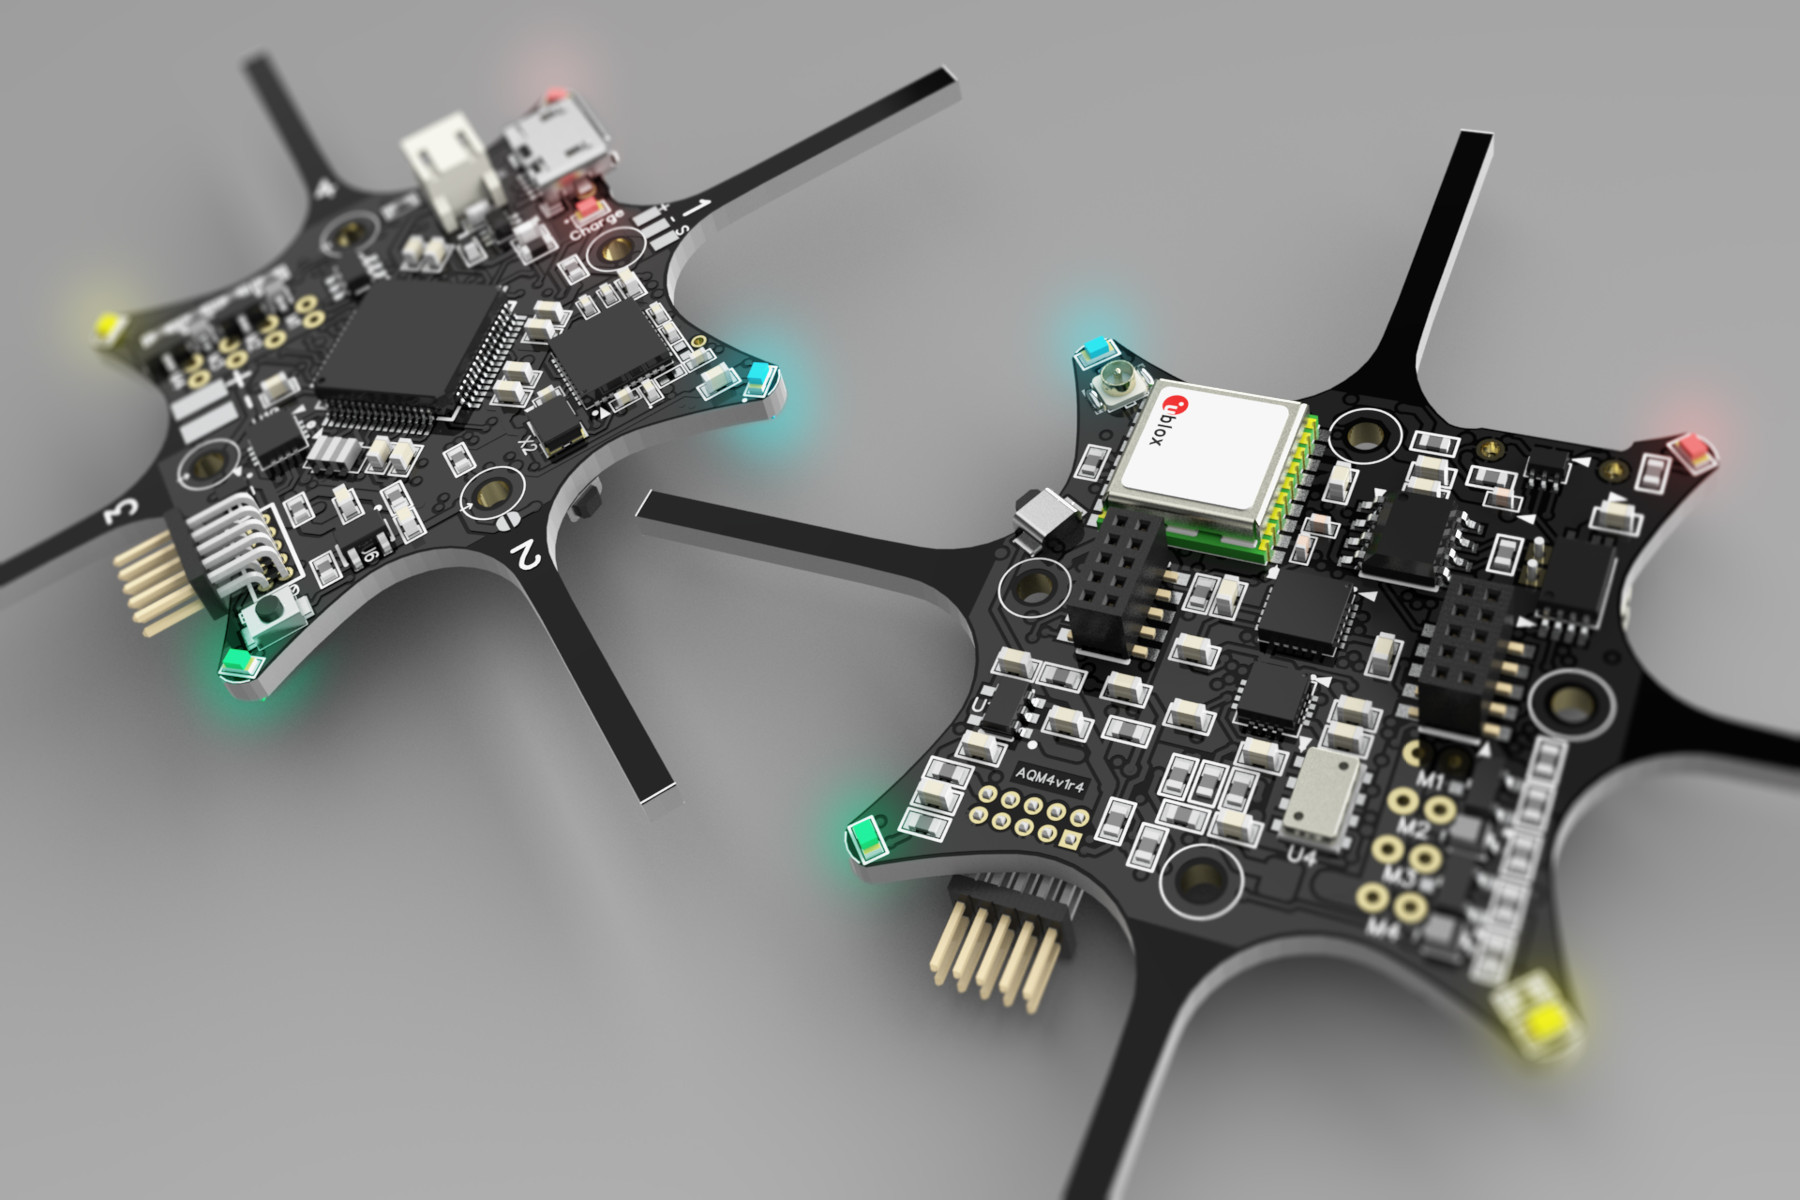
\includegraphics[width=\textwidth]{graphics/M4_demo}
        \caption{M4 flight pilot}
        \label{fig:gull}
    \end{subfigure}
    ~ %add desired spacing between images, e. g. ~, \quad, \qquad, \hfill etc. 
      %(or a blank line to force the subfigure onto a new line)
    \begin{subfigure}[b]{0.3\textwidth}
        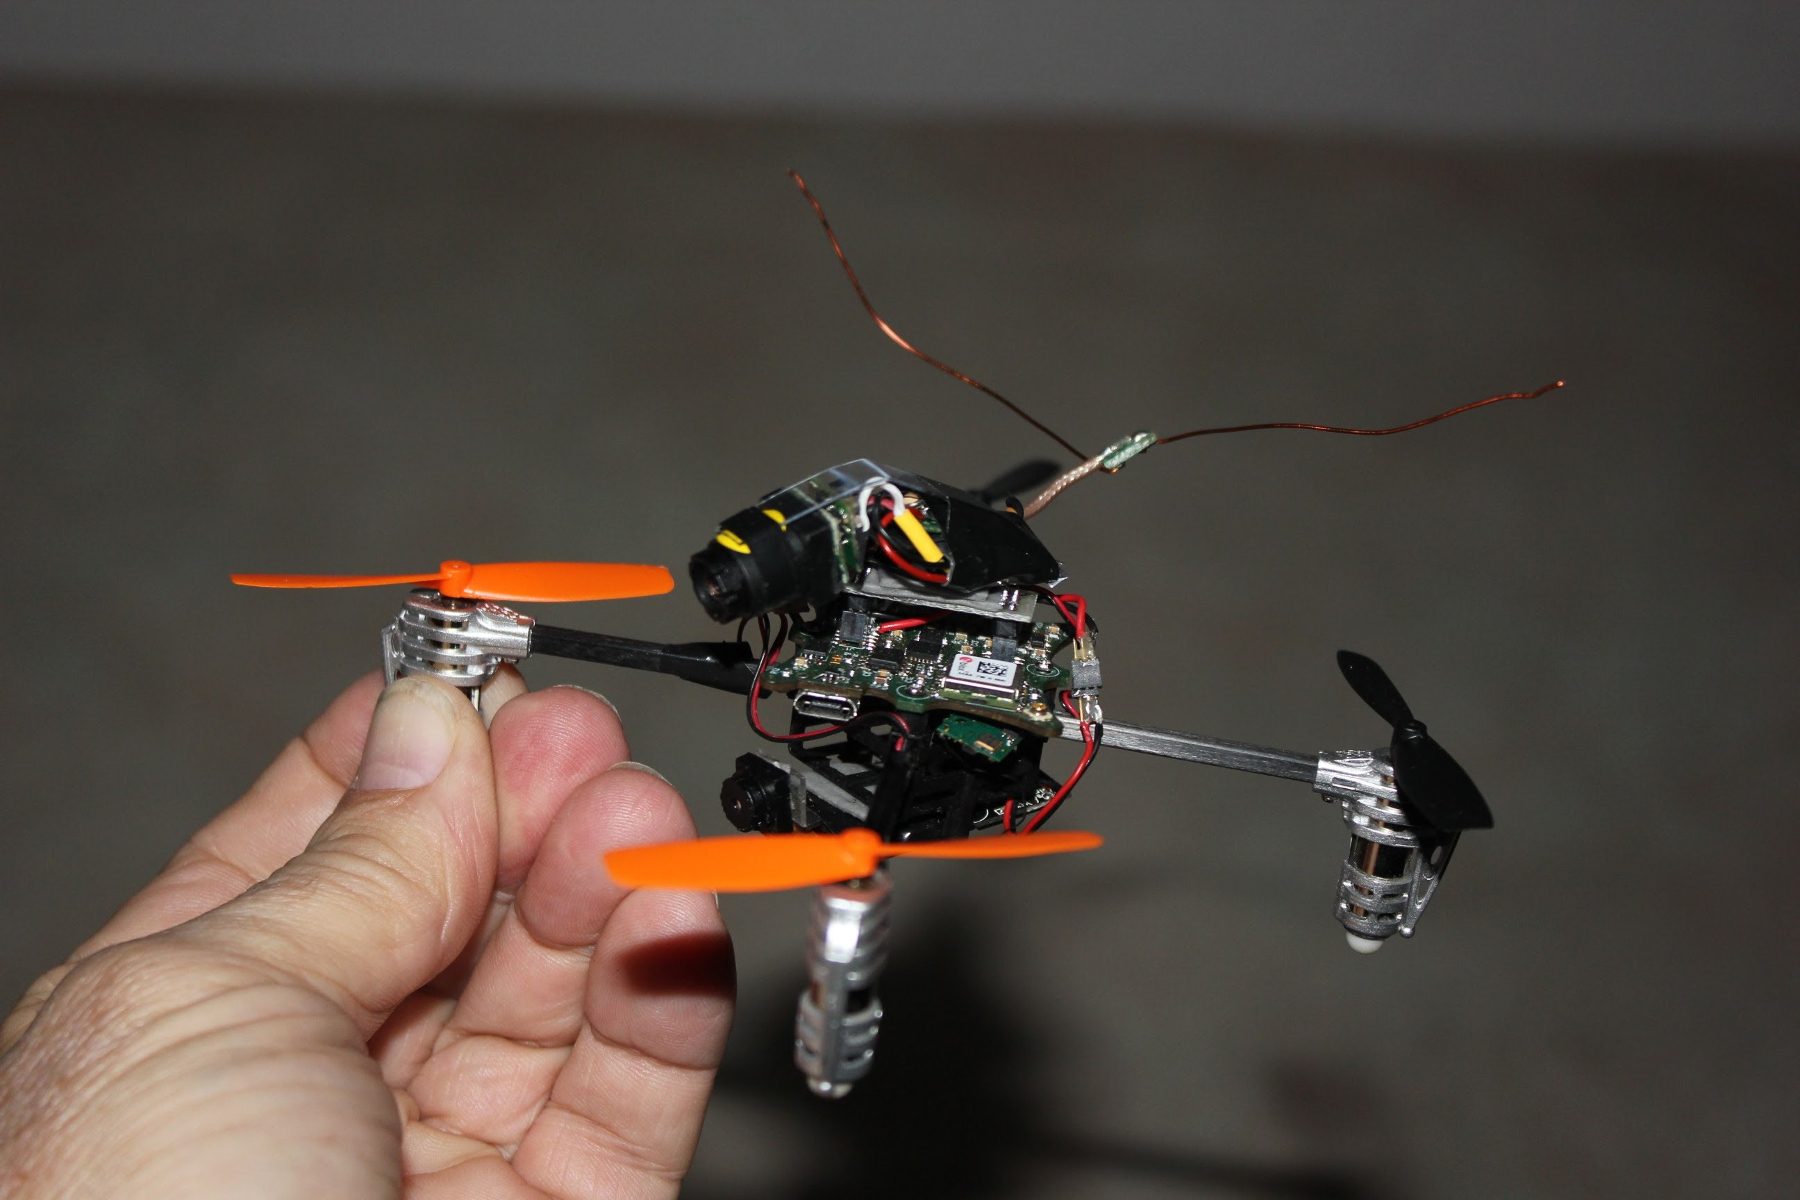
\includegraphics[width=\textwidth]{graphics/ladybird}
        \caption{Ladybird with mounted M4}
        \label{fig:tiger}
    \end{subfigure}
    ~ %add desired spacing between images, e. g. ~, \quad, \qquad, \hfill etc. 
    %(or a blank line to force the subfigure onto a new line)
    \begin{subfigure}[b]{0.3\textwidth}
        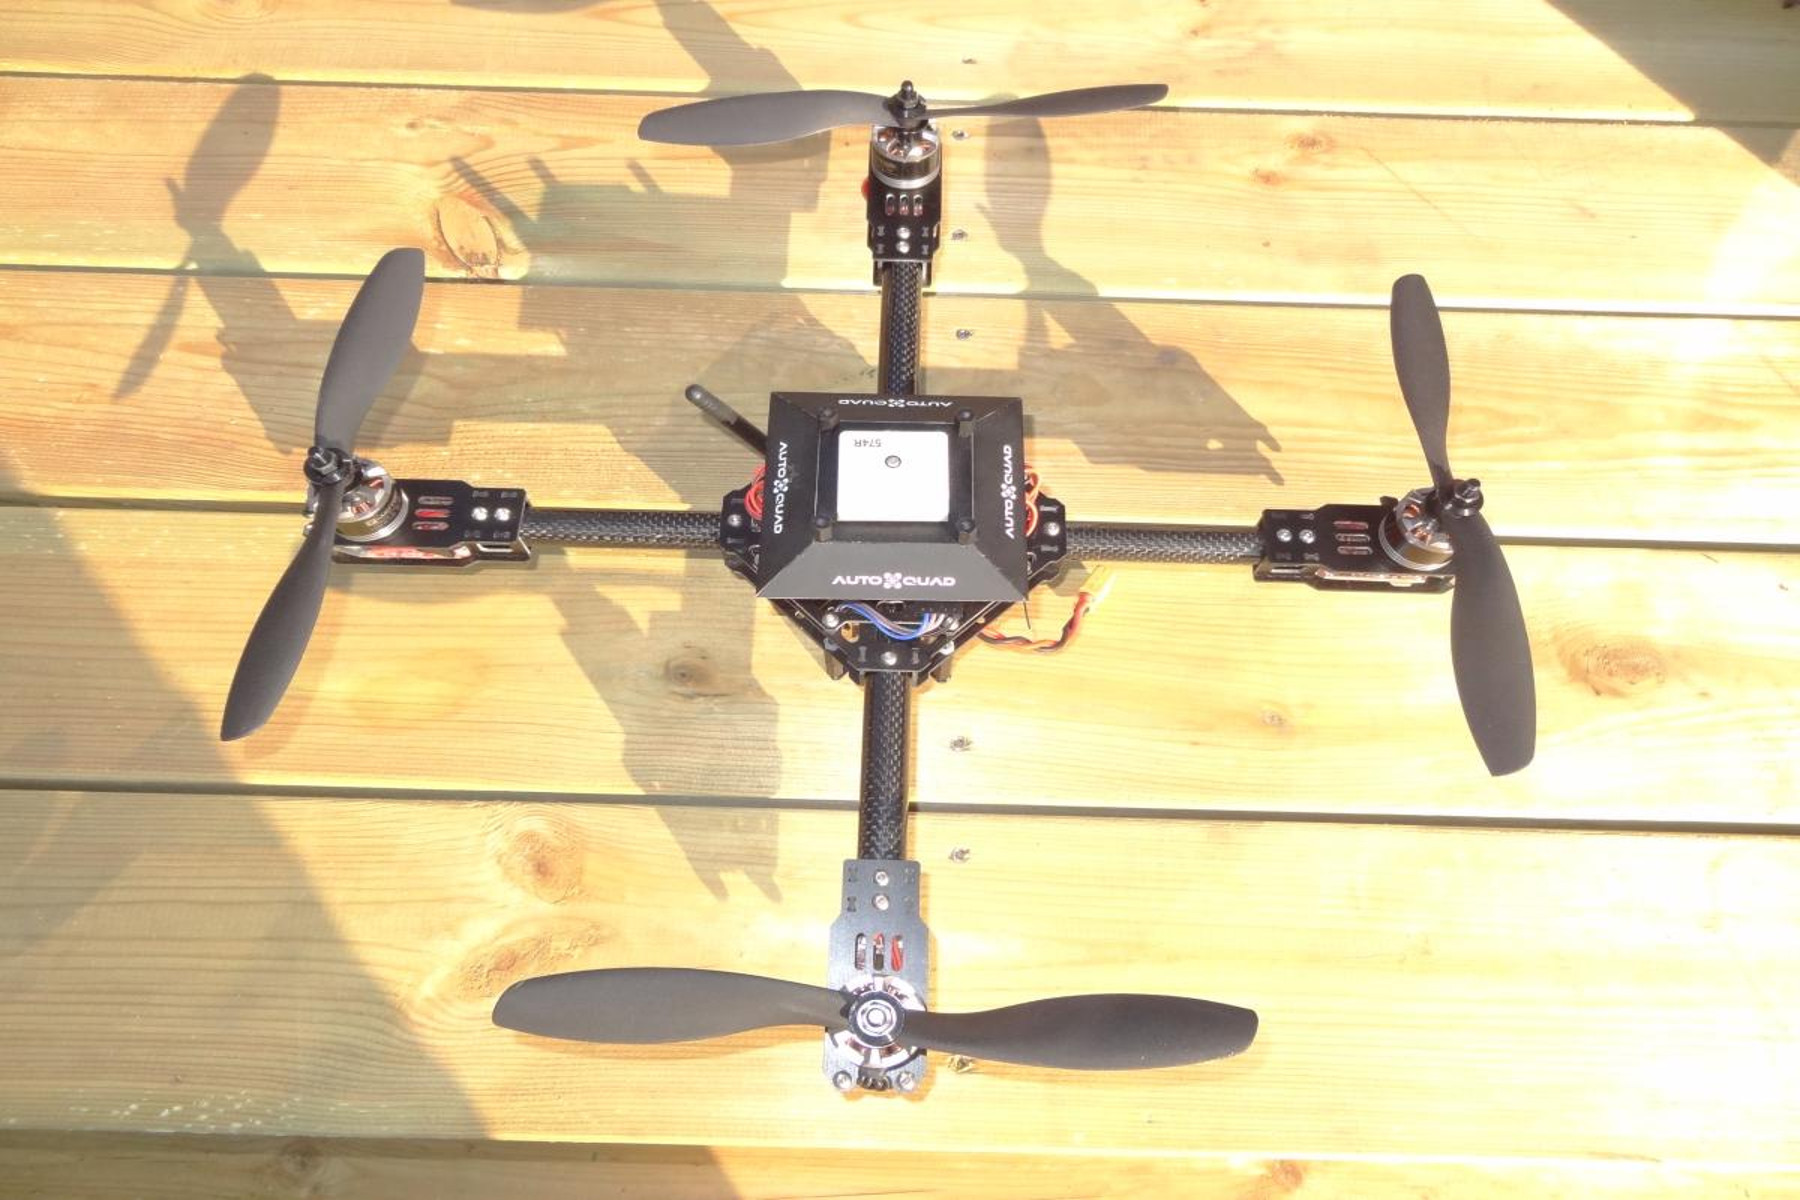
\includegraphics[width=\textwidth]{graphics/eduquad.jpg}
        \caption{Eduquad with M4 + ESC32}
        \label{fig:mouse}
    \end{subfigure}
    \caption{Pictures of AutoQuad hardware}\label{fig:AQ_hw}
\end{figure} 

At the time of writing, SDU is collaborating with HCA airport to find anomalies in fences.\\ 
\textit{Airports are burdened by a number of required inspection tasks to maintain a high level of 
safety and security.
Some of these tasks may advantageously be performed by a drone rather than the current manual labour, and this will save significant resources.
In this project they are targeting a specific need for frequent inspection of the fence surrounding the airport shown in figure \ref{fig:hca_fence}. 
The inspection concerns fence holes or similar anomalies. We hypothesize that a drone is 
capable of unsupervised autonomous inspecting the airport fence detecting small holes down 
to a radius of 5 cm.} \footnote{Application sent to Energi Fyns Udviklingsfond which has been granted, Ansøgning 2015-01-30 Energi Fyns Udviklingsfond-1.pdf on USB}

\begin{figure}[H]
    \centering
    %(or a blank line to force the subfigure onto a new line)
    \begin{subfigure}[b]{0.45\textwidth}
        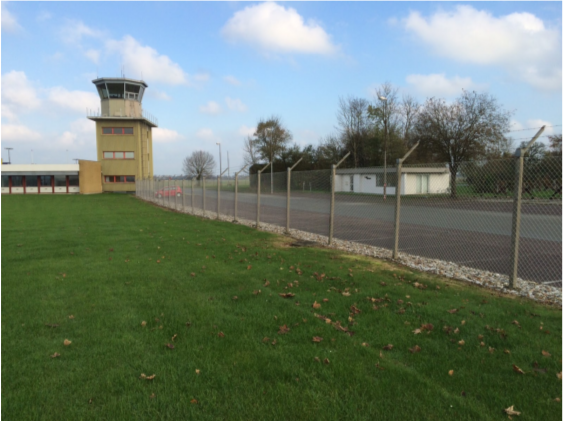
\includegraphics[width=\textwidth]{graphics/hca_fence.png}
        \caption{Part of the fence surrounding HCA Airport.}
        \label{fig:hca_fence}
    \end{subfigure}
        ~  %add desired spacing between images, e. g. ~, \quad, \qquad, \hfill etc. 
    %(or a blank line to force the subfigure onto a new line)
    \begin{subfigure}[b]{0.45\textwidth}
        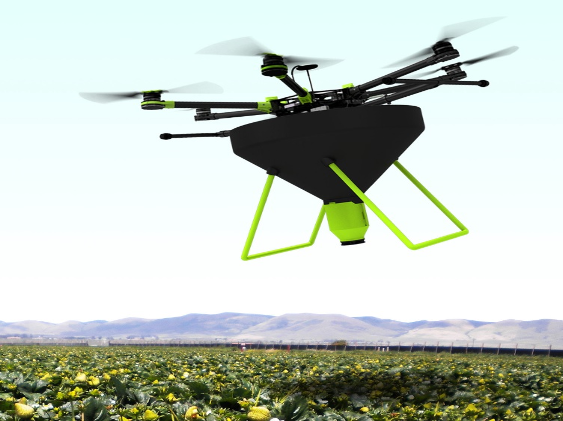
\includegraphics[width=\textwidth]{graphics/organicdrone.png}
        \caption{Drone spreading ladybirds and gall midges}
        \label{fig:organicdrone}
    \end{subfigure}
   \label{fig:sdu_projects}
\end{figure}
\Mathias{Huske at skrive hvem der støtter projekt samt med hvor meget de er støttet}
In order to avoid flying into the fence and to fly accurate enough for the camera to film, it is required to use an RTK GPS\footcite{2_gakstatter_2014}.

In another project, SDU is working together with a company, Ecobotix, to avoid the need of pesticides in organic crops. Pesticides are used to kill pests from the crows. When using pesticides a health risks exists for those who eat the crops. The use of pesticides also reduce the amount of diversity in nature since it is also killing beneficial organisms and potentially harm other animals in the food chain like birds. If nothing is used the crops might die, and that is very expensive to the farmer. \footnote{\url{http://naturerhverv.dk/tvaergaaende/gudp/gudp-projekter/2015/oekodrone-skal-sprede-mariehoens-i-stedet-for-pesticider/} last visited 18-04-2016}\\
SDU and Ecobix use drones to spread bugs like ladybirds and gall midges, over the crops to eat pests as shown in fugure \ref{fig:organicdrone}. \\
It is required the drones fly approximately 1 meter above ground at 1.5 meter/sec. It is therefore necessary to use an RTK-GPS in order to avoid hitting the ground in case of pumps in the fields. \footnote{Jensen, K.; Larsen, R.; Laursen M.S.; Neerup, M.M.; Skriver, M. and Jørgensen, R.N. Towards UAV contour flight over agricultural fields using RTK-GNSS and a Digital Height Model. Accepted for oral presentation at CIGR-AgEng June 2016.}\\
Both projects tends to use AutoQaud to solve their tasks. The AutoQuad version available at the moment of writing only supports autonomous flying using its onboard GPS. This project extends AutoQuads functionality by making it support global positioning from an RTK-GPS. 

\newpage
\subsection{Problem Statement}
The current AutoQuad version does not support any other source of global positioning than the onboard GPS and thereby does not support accurate flying better than GPS and if GPS is not available, there i is no alternatives supported. For AutoQuad to be used in applications requiring high accuracy or where GPS is unavailable this functionality is needed. \\


\subsection{Related Work}
In order to find relevant research about drones flying indoor, a few search phrases was conducted.
The following keywords were used to create different phases: Indoor, environment, swarm, localization, AutoQuad, quadrotor, mini UAV, test facilities, ETH, accurate, RTK, totalstation.
Based on the keywords a few papers was deemed relevant to the project and has been combined in order to give the reader an overview within the field of this project. \\

Developers of AutoQuad did previously try to implement RTKLib \footnote{http://www.rtklib.com} in AQ. Unfortunately they did manage to make it work as expected \footnote{Jussi Hermansen, owner of \url{http://ViaCopter.eu}}.\\

One of the big players within the field of indoor navigation and controlling multiple drones accurately is the university ETHzûrich and their Institute for Dynamic Systems and Modelling \footnote{\url{http://www.idsc.ethz.ch/research-dandrea/research-projects/aerial-construction.html}}. They have developed a test flying area they call "Flying Machine area" which provides facilities for doing prototype testing of new control algorithms \cite{lupashin2014platform}. The FMAs dimensions is 10*10*10m and provides nets to protect people and mattresses to protect the drone  if a crash. The FMA has further been developed into a mobile installation to be used in demonstrations in Europe and North America. One of their demonstrations where used in a TED video about multiroters and their capabilities \footnote{https://www.ted.com/talks/raffaello\_d\_andrea\_the\_astounding\_athletic\_power\_of\_quadcopters}.
The multiroter usually used in the FMA is Ascending Technologies' Hummingbird with custom wireless communication and electronics. \\
They have build it as a module design in order to be easy to replace parts of their system by simulations and to make it scalable.
One of their modules is a copilot that implements an accident handler in case of user-code crashing or sending invalid commands to the drones.
They are using UDP multicast packets as communication between ground computation and flying objects. The use of UDP multicast packets between modules since to makes the system more simple but also to avoid the need of buffers to handle unsuccessful transmissions and retransmissions. \\
In order to detect the quadroters they are using a commercial motion capture system. Three reflective markers is mounted on each flying object in order to obtain attitude and position. They are using three cameras to reduce the risk of false positive even though two cameras would be enough to get a flying objects 6D position.\\
 
 
\cite{kang2015indoor} proposes a more simplistic approaches to do indoor navigation.
They use bluetooth 4 to communicate between their multiroter(Rolling Spider) and an android phone which controls the multiroter.
They have mounted a camera on the ceiling to detect the target and the flying multiroter.
By doing background subtraction they can detect where the drone is in the frame by subtracting the background from each frame \cite{wikiBackgroundsubtraction}. 
By doing a convolution sum, the targets can be located. By analyzing the pixels around the location of the multiroter, they can get the heading. \\

\cite{sanchez2014system} proposes a framework to accelerate the process of prototyping multiroters behaviors. Their framework is designed for a swarm of drones to fly in a environment with obstacles. One of their design requirements is, that the framework should be highly decoupled from the application the researcher is testing in order to speed up the development process. 
Position estimates is obtain by using onboard IMU and optic flow. To avoid expensive motion capture systems they have used markers that can easily be recognized by cameras mounted on the drones to get a absolute 3D estimate. Each obstacle got a ArUco-marker \cite{Aruco2014} that can be detected by the front camera mounted on the multiroter. \\
They have decided to use ROS as middleware to provide generic interfaces between the modules used in their framework. Different multiroters can be used as long they use the same interface. Communication between multiroters and ground station(if used) is done using WIFI. \\


The most common type of indoor localization is using vision where the camera is either mounted in the environment or where the drone is equipped with cameras to obtain position estimates.\\
\cite{stirling2012indoor} uses a different approach where they use a \textit{Robot Sensor Network} to map the environment.
The idea is that each drone can either be a beacon or explorer. Each drone alternates between these two states. Beacons stays still below the ceiling without moving while explorer flies around to unknown locations. Beacons emit IR light in order to triangulate beacons position.  Beacons detecting unexplored locations calls for explorer that will become beacons and so forth until the environment is mapped. To synchronize the beacons 2.4 ghz WIFI is used. When the environment is mapped, graph searching algorithms can be used to find a path through the environment.


\subsection{Hypothesis}
If each drone's 2D position is obtained using vision and spoofed into the drone using CAN, then it is possible for at least 3 drones to follow a leader drone with a preprogrammed flight path and keep a euclidean distance at 50 cm within plus minus 10 cm to the leader and its neighbours.
\subsection{Aim of project}
The aim of this project is to test the hypothesis by making an indoor flying environment to make 3 multirotors follow a leader multirotor. Since a need from SDU has arisen of sending RTK GPS coordinates into AutoQuad, this will also be used to test and to contribute to a scientific paper.



\chapter{Materials and methods}
\textit{This chapter concerns the most important parts about how this project has been implemented. It has been split into several sections.}

\newpage
\section{System architecture}
\textit{This section describes the overall system architecture indoor as well as outdoor. The section goes in details with the components used and how they are connected. Furthermore it describes the information flow through the system. The design choices and implementation details will be covered later in this chapter.}

The section has been split into two subsections in order to address indoor and outdoor positioning separately.

\subsection{Indoor} \label{sec:system_architecture_indoor}
Figure \ref{fig:indoor_information_flow} shows the system architecture for indoor positioning. The laptop detects the drones position using vision, sends it through the ROS nodes and transmits the GPS positions to the drones via WIFI.
Each drone receives its position and sends it into the M4 flight controller over \ac{CAN}.
\begin{figure}[H]
    \center
    \includegraphics[width=1\textwidth]{graphics/system_architecture_indoor_all.png}
    \caption{Diagram showing system architecture when used indoor. The markers used to track the drones is shown below the camera.}
    \label{fig:indoor_information_flow}
\end{figure} 

A Logiteh C930 camera\footnote{The camera is used in other courses to track mobile robots so the author did not have any influence on which camera to use} was mounted below the ceiling to detect the drones when flying. The order of the marker of each drone is unique in order to identify the particular position of the drone.


\subsubsection*{ROS}
\ac{ROS}\footnote{http://www.ros.org/} is used as middleware on the laptop as inter-process communication. By using ROS it is easier to debug since each node\footnote{Process in \ac{ROS} terminology} can be isolated and debugged without everything has to be connected. \ac{ROS} uses subscriber-publisher pattern which means one or more nodes can produce data, and one or more nodes can consume data. Topic is the term used to define a communication channel between nodes. Nodes producing data are referred to as publishers, and nodes consuming data are referred to as subscribers.
Furthermore \ac{ROS} supports running nodes distributed across multiple PCs meaning the MarkerLocators can be distributed if more CPU resources are needed when tracking several drones.
The squares shown in the \ac{ROS} section in figure \ref{fig:indoor_information_flow} shows the \ac{ROS} nodes and how they are connected using topics.


\begin{itemize}
	\item \textit{cam\_to\_topic} captures frames from the Logitech camera and publish the raw frame to \textit{/camera/down} as a RGB picture.
	\item \textit{MarkerLocator\_trackN} subscribes to \textit{cam\_to\_topic} and processes the frame in order to localize the marker or order N of the drone in the frame. This node publishes messages to \textit{/positions/droneN} containing x,y position, orientation and a boolean telling whether the right marker is found in the frame or not. The MarkerLocator was customized to support receiving frames from a topic instead of the camera directly. By doing this, multiple instances of the MarkerLocator can be run in parallel without their performance impact each other. \footnote{Indoor localization is described in section \ref{sec:indoor_localization}}
	\item \textit{Decision\_Maker} subscribes to the topics containing the position of the drones. This node publishes messages to \textit{/communication/to\_droneN} containing the \ac{LLH} position of the drone. This node contains the logic for controlling the drones \footnote{Decision\_maker is described in section \ref{sec:control_and_coordinate_conversion}}. Due to the modularity of ROS, changing the behavior of the drones is a matter of replacing this node.
	\item \textit{wifi\_outN} subscribes to \textit{/communication/to\_droneN} and transmits the received messages to the drone using WIFI. The responsibility of this node is to pack the message, calculate \ac{CRC}, append it and send it as an \ac{UDP} packet. The content of the frame can be seen in table \ref{tab:wifi_frame}.
\end{itemize}

\begin{table}[H]
\centering
\begin{tabular}{@{}|l|l|l|l|l|l|l|l|l|l|@{}}
\toprule
\textit{Content}  & CRC-16    & Future  & eDOP  & nDOP & tDOP & vDOP &      Height   & Lon     & Lat       \\ \midrule
\textit{Datatype} & uint16\_t & 4 byte  & byte  & byte & byte & byte &      double   & double  & double  \\ \midrule
\textit{Bytes}    & 33:32     &  31:28  & 27    & 26   & 25   & 24   &      23:16    & 15:8    & 7:0       \\ \bottomrule
\end{tabular}
\caption{Table shows the frame sent from the \textit{wifi\_out\_N} to the extension-boards. 4 bytes is not utilized but can be used for anything or the frame can be reduced in size}
\label{tab:wifi_frame}
\end{table}

The frame in table \ref{tab:wifi_frame} is 34 bytes long but can be enlarged or made smaller if needed. However the ESP8266 module has a limitation of 8192 bytes \footnote{\url{https://github.com/esp8266/Arduino/blob/master/libraries/ESP8266WiFi/src/WiFiUdp.h\#L28} last visited 28 Maj}

The initial idea was to also send the velocities of the drone and the accuracies to each extension-board since this information is used by AQ M4, however due to lack of time this was not implemented.

\subsubsection*{Drone} \label{sec:system_indoor_drone}
The drone is a Ladybird using a \ac{AQ} M4 as flight controller with a modified version of the firmware.\footnote{AQ M4 firmware is described in section \ref{sec:aq_m4_firmware}} Is has an extension-board that enables it to receive positions from WIFI and inject them into the \ac{AQ} M4 over \ac{CAN}. \footnote{The extension-board is described in section \ref{sec:autoquad_extension_board}}
\begin{itemize}
	\item \textit{ESP8266}\footnote{The firmware running on the ESP8266 module is described in section \ref{sec:exp8266_firmware}} receives the UDP packet sent from the computer running \ac{ROS}. When a frame is received, it checks if the received number of bytes it correct. If so, it encapsulates the packet using \ac{SLIP} and transmit it to the At90CAN128.
	\item \textit{At90CAN128} receives the encapsulated packet, decapsulate it, verify the CRC and transmit the packet to the \ac{AQ} M4 over \ac{CAN}. Tables \cref{tab:CAN_DOC_LAT,tab:CAN_DOC_LON,tab:CAN_DOC_VEL,tab:CAN_DOC_ALT,tab:CAN_DOC_DOP,tab:CAN_DOC_ACC} show the CAN-messages send to the \ac{AQ} M4.
\end{itemize}


\begin{multicols}{2}
\begin{table}[H]
	\begin{tabular}{@{}|l|l|@{}}
		\toprule
		DOC   & CAN\_DOC\_LAT \\ \midrule
		Value & Latitude      \\ \midrule
		Bits  & 63:0          \\ \bottomrule
	\end{tabular}
	\caption{CAN message to \ac{AQ} containing 8 byte latitude}	\label{tab:CAN_DOC_LAT}

	\begin{tabular}{@{}|l|l|@{}}
	\toprule
		DOC   & CAN\_DOC\_LON \\ \midrule
		Value & Longitude     \\ \midrule
		Bits  & 63:0          \\ \bottomrule
	\end{tabular}
	\caption{CAN message to \ac{AQ} containing 8 byte longitude} 	\label{tab:CAN_DOC_LON}

\end{table}
\columnbreak
\begin{table}[H]
	\begin{tabular}{@{}|l|l|l|l|l|@{}}
		\toprule
		DOC   & \multicolumn{4}{l|}{CAN\_DOC\_VEL} \\ \midrule
		Value & VelN    & VelE   & VelD   & speed  \\ \midrule
		Bits  & 63:48   & 47:32  & 31:16  & 15:0   \\ \bottomrule
	\end{tabular}
	\caption{CAN message to \ac{AQ} containing velocities each of 2 bytes}
	\label{tab:CAN_DOC_VEL}
	\begin{tabular}{@{}|l|l|@{}}
	\toprule
		DOC   & CAN\_DOC\_ALT \\ \midrule
		Value & Altitude      \\ \midrule
		Bits  & 63:0          \\ \bottomrule
	\end{tabular}
	\caption{CAN message to \ac{AQ} containing 8 byte altitude}
	\label{tab:CAN_DOC_ALT}
\end{table}
\end{multicols}

\begin{table}[H]
	\begin{tabular}{@{}|l|l|l|l|l|l|l|l|@{}}
		\toprule
		DOC   & \multicolumn{7}{l|}{CAN\_DOC\_DOP}                  \\ \midrule
		Value & gDOP  & eDOP  & nDOP  & tDOP  & vDOP  & hDOP & pDOP \\ \midrule
		Bits  & 55:48 & 47:40 & 39:32 & 31:24 & 23:16 & 15:8 & 7:0  \\ \bottomrule
	\end{tabular}
	\caption{CAN messages to \ac{AQ} containing \ac{DOP}s each of 1 byte}
	\label{tab:CAN_DOC_DOP}
	\begin{tabular}{@{}|l|l|l|l|l|l|l|l|@{}}
		\toprule
		DOC   & \multicolumn{7}{l|}{CAN\_DOC\_ACC}                          \\ \midrule
		Value & Heading & vAcc  & hAcc  & cAcc  & sAcc  & Fix  & Satellites \\ \midrule
		Bits  & 63:48   & 47:40 & 39:32 & 31:24 & 23:16 & 15:8 & 7:0        \\ \bottomrule
	\end{tabular}\label{tab:CAN_DOC_ACC}
	\caption{CAN messages to \ac{AQ} containing accuracies of 1 byte and heading in 2 bytes} 
\end{table}

\subsubsection*{Network configuration}  \label{sec:network_configuration}
The WIFI  network for handling the communication between the PC and the drones had to be configured \footnote{Wireless communication chosen in  section \ref{sec:wireless_communication_module}}.
The PC was configured as an access point for each extension-board to join. The access point was setup using an Asus USB-N13\footnote{Not available on AUSUS' webpage.} netcard and hostapd\footnote{https://w1.fi/hostapd/} as software. The network was configured as \ac{WPA2} to make it difficult for other to connect and start messing with the network.

Instead of hardcoding an  \ac{IP} for each extension-board, which would be cumbersome each time a new firmware had to be deployed, a \ac{DHCP} server was configured on the PC. Since the IP might change next time the module connects, Multicast-DNS was configured on the ESP8266 and the PC. Each extension-board was giving a hostname eg. Drone1 so when the PC has to send a frame to Drone1, the underlaying networking will resolve the IP of Drone1.
The ESP8266 has a small filesystem build-in which support creating a configuration file that could contain the hostname.
When flashing the ESP8266 module the configuration file\footnote{Due to lack of time the configuration file was not made, and the hostname was hardcoded in the ESP8266 firmware.} would not be overwritten and thereby still have the hostname of the module. Instead of using hostnames the \ac{IP} of the drone could be entered in the configuration file, however this would make it less portable since the PC would always have to be on the same \ac{IP}-range.


\subsection{Outdoor}
\begin{figure}[H]
    \center
    \includegraphics[width=0.7\textwidth]{graphics/system_architecture_outdoor.png}
    \caption{Diagram shows information flow when used outdoor. The RTK-GNSS provides a absolute position which is read and converted to CAN messages by the Raspberry PI}
    \label{fig:outdoor_information_flow}
\end{figure}

The \ac{RPi} is also running \ac{ROS} since it uses two components from Frobomind\footnote{\url {http://frobomind.org/} last visited 29 Maj}. \begin{itemize}
	\item \textit{serial\_nmea\_node} is used to read and write from the serial port. Further more it decodes the NMEA string sent by the \ac{RTK-GNSS}
	\item \textit{can\_socket\_node} is used to communicate with the \ac{CAN}-adapter\footnote{PEAK-CAN Adapter has been used in this project}
\end{itemize}

When a GPGGA/GPRMC nmea \footnote{\url{http://www.gpsinformation.org/dale/nmea.htm} last visited 28 Maj} message is received from the \ac{RTK-GNSS} its read by the \textit{serial\_nmea\_node} node. It is then sent to the \textit{AQ\_msg\_conv} node which simply converts the content of the GPGGA/GPRMC to CAN-messages shown in \cref{tab:CAN_DOC_LAT,tab:CAN_DOC_LON,tab:CAN_DOC_VEL,tab:CAN_DOC_ALT,tab:CAN_DOC_DOP,tab:CAN_DOC_ACC}  . \\

Even though the positioning is shown using vision and \ac{RTK-GNSS}, other sources of positioning can be used as well. The same code is running on the \ac{AQ} M4 whether vision or \ac{RTK-GNSS} is used, so if other positioning systems should be used one should implement the \ac{CAN} protocol shown in appendix \ref{app:aq_can_protocol}.
If using \ac{CAN} is not possible a \ac{RPi} and \ac{CAN}-adapter can be used as intermediate, but then the \textit{serial\_nmea\_node} and \textit{AQ\_msg\_conv} should be replaced.

\newpage

\section{AutoQuad extension board} \label{sec:autoquad_extension_board}
\subsection{Introduction}
This secion will go in depth about the extentionboard created as an addon to the AQ M4 board. The extentionboard was developed to act as a bridge between the PC and the CAN-bus using wireless communication.\\
v
The block schematic shown in figure \ref{fig:PCB_block} was created by the auther of the report. It was then given to Carsten Albertsen who created the schematic and did rest of the creation of the PCB.
\\
\subsection{Block schmeatic}
\Mathias{Create schematic appendix}
\Mathias{Add GPS, WIFI, PCB, PC to forkortelses liste}
\Mathias{Thanks to Carsten Albertsen for PCB development}
\begin{figure}[H]
    \center
    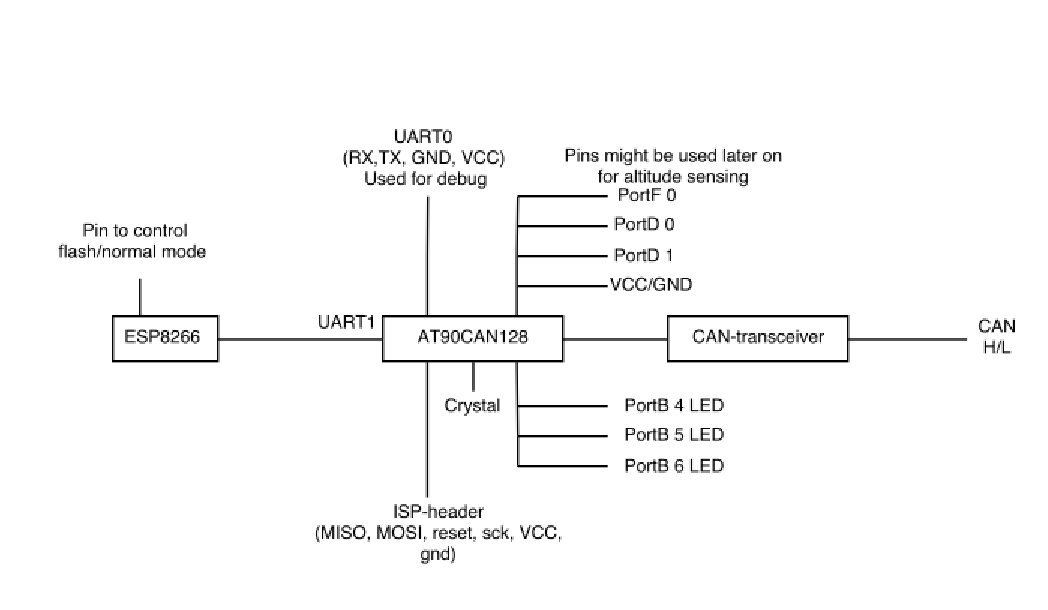
\includegraphics[width=1\textwidth]{graphics/PCB_block_v3.eps}
    \caption{Block schematic of the WIFI-extentionboard developed to AQ M4}
    \label{fig:PCB_block}
\end{figure}

\subsubsection{ATmega}
\subsubsection{Wireless Communication}
An important part of the hardware is the wireless communication used between the PC and the drones.
The wireless communication module has severel requirements it needs to fulfill in order to make the whole system work as expected. A comparison table has been made in table \ref{tab:compare_table_wireless_communication} to find the wireless communication module that is best suited for the task. \\
The following wireless modules where considered and compared.
\begin{itemize}
	\item \textbf{ESP8266}
\end{itemize}

ESP8266 is a generel purpose 32 bit SOC with integrated WIFI 802.11 b/g/n support and buildin TCP/IP stack. It can be setup its own access point or it can connect to an existing wireless network.
It runs at 80MHz and can be flashed with a custom firmware. 
The SOC is sold as modules with different pinouts and features such as extra flash memory \footnote{\url{https://www.olimex.com/Products/IoT/MOD-WIFI-ESP8266/open-source-hardware}} and different antennas.
The chip has been on the marked for about two years and costs approximately 7\$. 
It has been widely used in DIY-projects due to its low price and because it requires a minimum of network knowledge to get up and running.\footnote{\url{http://www.esp8266.com/} - 43.000 posts in forum} When the SOC is shipped, it comes with a preloaded firmware which either accepts AT commands or LUA scripting depending on the version of the module. These simple programming interfaces makes it quick and easy to interface the cheap. \\
This leads to a large community where most of the problems have been found and solved already. Arduino has been ported to ESP8266 which makes it even easier to get it up and running. Their official Arduino GitHub has 2125 commits on their master branch at the time of writing\footnote{\url{https://github.com/esp8266/Arduino}} \\

\begin{itemize}
	\item \textbf{EMW3165}
\end{itemize}
EMW3165 is a SOC much like the ESP8266 supporting 802.11 b/g/n WIFI with buildin TCP/IP stack. As with ESP8266 it supports setting up an access point aswell as connecting to an existing network. It has a Cortex-M4 $\mu$C which run at 100MHz. 
It supports custom firmware and can be aswell be bought as different modules with different pinouts and antennas.
It differentiates itself from the ESP8266 by its higher frequency its 5 volts compatible pins \footnote{\url{https://hackadaycom.files.wordpress.com/2015/07/emw3165.pdf}} which makes it easier to connect other hardware which run 5 volt without the need of a logic level shifter. It has been on the marked for only one year and costs approximately 9\$. Since it is a newer board than ESP8266 it has not been used in the same number of applications and thereby has a smaller community behind\footnote{\url{http://www.emw3165.com/} - 200 posts in forum }. Their most active GitHub has 147 commits on their master branch at the time of writing\footnote{\url{https://github.com/SmartArduino/WiFiMCU}}.

\begin{itemize}
	\item \textbf{nRF51822}
\end{itemize}
nRF51822 is also a SOC, but it is using Bluetooth instead of WIFI. The nRF51822 $\mu$C is implementing BLE which is a power efficient way of sending and receiving data. The chip supports broadcasting which could be used in this project. The $\mu$C can be bought as a standalone component or mounted on modules as the two other $\mu$Cs. Different modules offers different types of antenna connectors or buildin antenna on the PCB. It has not been possible to find an Arduino ported firmware that supports this $\mu$C. To write a firmware for the $\mu$C it has to be done using Nordic Semiconductor's proprietary SDK. 


\begin{itemize}
	\item \textbf{XBee}
\end{itemize}
XBee is a module that implements the Zbee standard. The Xbee modules work as a wireless serial connection. The Xbee modules supports mesh networking which means the modules by themself figure out which module is closest and makes the connection. This idea makes sense in this application since there will be multiple drones and one computer. If one drone gets too far from the PC, it can just connect to one of the other drones closer to the PC.\\
The Xbee solution is ready to use and requires a minimum of programming to get up and running. The modules also support GPIO for digital in and output and analog input.

\Mathias{ '\'footmotemark til at referere til samme fodnote flere gange}
\begin{table}[H]
	\centering
	\begin{tabular}{@{}|l|l|l|l|l|l|l|l|@{}}
		\toprule
		\textbf{Product} & \textbf{Size} & \textbf{Weight} & \textbf{Price} & \textbf{Documentation} &  \textbf{Range}  & \textbf{Score} \\ \midrule
		ESP8266   &  24x16mm\footnote{\url{https://www.mikrocontroller.net/attachment/243558/fcc\_11.pdf}} \hfill\{7\} & 1.5g\footnote{Measured by author on chemistry weight} \hfill\{8\} &   7.5\$\footnote{\url{http://www.seeedstudio.com/depot/ESP8266-based-WiFi-module-SPI-supported-p-2486.html}}    &   Great community \hfill\{9\}  &    ?    &                		\\ \midrule
		EMW3165   &  32x16mm\footnote{\url{https://hackadaycom.files.wordpress.com/2015/07/emw3165.pdf}} \hfill\{6\}  & 5g\footnote{\url{http://www.seeedstudio.com/depot/EMW3165-CortexM4-based-WiFi-SoC-Module-p-2488.html}} \hfill\{2\} &  9\$\footnote{\url{http://www.seeedstudio.com/depot/EMW3165-CortexM4-based-WiFi-SoC-Module-p-2488.html}}   &  Less available  \hfill\{3\}	        &    ?    &                		\\ \midrule
		nRF51822  &  18x10mm\footnote{\url{http://www.fanstel.com/Product/bluenor.html}} \hfill\{8\}  & 3g\footnote{\url{http://www.seeedstudio.com/depot/MDBT40P\%C2\%A0\%C2\%A0nRF51822\%C2\%A0based\%C2\%A0BLE\%C2\%A0module-p-2503.html}} \hfill\{0\}  &  7.5\$  & Ok documented\hfill\{2\} 	        &   30 M\footnote{\url{https://dl.dropboxusercontent.com/u/54939426/Fanstel_BT600.pdf}}  \hfill\{9\}     &                		\\ \midrule
		XBee      &  24.38x27.61mm \footnote{\url{http://www.digi.com/products/xbee-rf-solutions/modules/xbee-802-15-4\#specifications}} \{3\} & 3g \footnote{\url{http://www.digi.com/products/xbee-rf-solutions/modules/xbee-802-15-4\#specifications}} \hfill\{4\} &   25\$\footnote{\url{https://www.sparkfun.com/products/11215}}    &  Lots of DIY   \hfill\{9\}      &            91 M\footnote{\url{https://www.sparkfun.com/pages/xbee_guide}}  \hfill\{9\}  &                    \\ \bottomrule
	\end{tabular}
	\caption{Comparisontable used to compare different wireless 		communication modules}
	\label{tab:compare_table_wireless_communication}
\end{table}
\Mathias{vægt på ESP til 3 gram med link - det er hvad der er oplyst. Efterfølgende skrive at det er vejet til 1.51 gram(hen mod slutningen)}
The products compared in \ref{tab:compare_table_wireless_communication} are chosen to have approximately same specs. Onboard antenna, breakout for easy pin access.

\subsubsection{Pins}
A few pins where made available through solder pads for easy access if needed later on.

The following pins where available as solder pads:
\begin{itemize}
	\item PortF 0 - Alternative function as ADC, channel 0
	\item PortD 0 - Alternative function as interrupt, INT0
	\item PortD 1 - Alternative function as interrupt, INT1
\end{itemize}
In case the onboard baromter isn't accurate enough, an alternative distance could be used to measure the drones altitude with respect to the ground.
PortF0 has been made available since some distance sensors give output as an analogue value. 
An example of such sensor is an Infrared proximity sensor.\footnote{\url{http://www.sharpsma.com/webfm\_send/1208}} \\
As an alternative type of distance sensor, a ultrasoinc could be used such as HCSR04.
As output it gives a binary output with high-time proportional with the distance.\footnote{\url{http://www.micropik.com/PDF/HCSR04.pdf}}.
To detect the high-time, one of PortD1/0 would be useful. \\

Which type of sensor suits best as a distance sensor to provice altitude information to the drone is ouf of the scope of this report. The PCB has just been made ready to different types of sensors.

\subsubsection{Debug/ISP}
In the final schematic UART0 and ISP pins where combined in one pinheader for easy access through one cable. \Mathias{Refer to image of board}
To program the AtMega the ISP pins where required to be easy accessable. 
UART0 was made accessable to be used as debug and programming of the ESP8266 board.
The plan was to setup the AtMega as UART passthrough from UART0 to UART1.
Due to a mistake\footnote{The wrong pair of MISO/MOSI pins where made available in the ISP-header. The correct pair of MISO/MOSI is also RXD0/TXD0 as alternative function} in the final schematic, both UART0 and UART1 where made accessable trough the ISP/debug header. 
This ended up making it easier to program the ESP8266-board without using the AtMega as UART passthrough.

ESP noteS:
 - GPIO15 = bootmode, low for ...
 - GPIO0 = flash mode
 
 
 https://zoetrope.io/tech-blog/esp8266-bootloader-modes-and-gpio-state-startup

\newpage

\section{AutoQuad extension board firmware}
\textit{In this chapter the development of the firmwares running on the extension board is described. Different types of schedulers for the At90CAN128 is discussed and a scheduler is chosen and developed with the required functionality. The communication between PC and M4 is further described. At the end of each section a test is conduced in order to show if the code works as expected }
\subsection{Scheduler}
\textit{This capter concerns only the Atmega.  The ESP module will be descriped in section \ref{sec:esp_firmware}} \\
In order to have a timing on the At90CAN128 a scheduler was chosen and implemented.
The list below shows 3 different types of scheduler that was considered.
\begin{itemize}
	\item Real-time Operating System(RTOS) provides strict timing but at the cost of overhead. A RTOS runs task in a "parallel" environment. Each task runs in a loop and the RTOS scheduler will do context switching when needed. Using a RTOS requires mutexes and semaphores to protect shared resources which increases the complexity and amount of overhead
	\item Super-Loop provides no timing at all, but process data as fast as possible. It does not do any context switching and does not require mutexes or semaphores and  and thereby takes no overhead.
	\item Run-To-Complete(RTCS) scheduler is a mix of the two other schedulers. It works by waiting for a tick generated by a hardware timer and then starts executing all tasks from the beginning. The order of the task matters if there is dependency between the tasks but also to make sure the task requiring the most precise timing is at the beginning of the list of the tasks. All tasks have to be finished executing before the next tick is giving in order to avoid timing is ruined.
\end{itemize}
The RTCS was chosen since it provides timing without the overhead created when doing context-switching and the need of mutex and semaphores. It further reduces the code-complexity.\\

It was decided to implement the code in tasks to make a low coupling between the functionalities. This makes it easier to maintain and expand later of if needed. The task diagram shown in figure \ref{fig:task_diagram_atmega} shows the tasks and how they do intertask communication.


\begin{figure}[H]
    \center
    \includegraphics[width=0.9\textwidth]{graphics/task_diagram.png}
  \label{fig:task_diagram_atmega}
  \caption{Tasks diagram showing overview of the running tasks on the At90Can128}
\end{figure}



\subsubsection*{Test of RTCS timing}
In order to test the timing of the scheduler, a led\_task was written. The task can be seen in code \ref{code:test_scheduler}
\begin{lstlisting}[language = c, caption = RTCS task used in timing test, label=code:test_scheduler]
void is_alive_task(uint8_t my_state){

	// Write to UART0
	UDR0 = my_state+'0';

	switch(my_state){
	case 0:
		INT_LED_ON_GREEN;
		INT_LED_OFF_RED;
		INT_LED_OFF_BLUE;
	    set_state( 1 );
		break;
	case 1:
		INT_LED_OFF_GREEN;
		INT_LED_ON_RED;
		INT_LED_OFF_BLUE;
	    set_state( 2 );
		break;
	case 2:
		INT_LED_OFF_GREEN;
		INT_LED_OFF_RED;
		INT_LED_ON_BLUE;

		// Set next state
	    set_state( 0 );
		break;
	}
	// Wait one second
	wait( 1000 );
}
\end{lstlisting}

The test was done by writing the current state of the task to UART0.\\ A python script were made that measures the time between each character received. The script can be seen in code \ref{code:test_rtcs_python}.
\begin{lstlisting}[language = python, caption = Python code used to measure time between received byte, label=code:test_rtcs_python]
#!/usr/bin/python
import serial
import time

ser = serial.Serial( port='/dev/ttyUSB0', baudrate=57600 )

t = time.time()
while True:
    for char in ser.read(1):
        print time.time() - t, ","
        t = time.time()

ser.close()
\end{lstlisting}
The output of the script were redirected to a file. After receiving 700 bytes the standard deviation and mean was calculated using matlab.
The mean is 1.0089 sec with a standard deviation of 0.0042 sec.

Part of the variance is caused by the inaccuracy of the timing on the PC running the python code. If a more accurate measure was needed, a scope could be attached to the $\mu$C's GPIO. Each time the scheduler enters the task the GPIO should be set high, and when it exists the GPIO should be set low. The scopes at SDU is capable of telling the variance of the off signal. \\
It can be concluded that the scheduler performs well.
\newpage

\subsection{Queues}
\subsection*{Test of CAN, queues}
In order to test CAN and queues, a task was written. The purpose of the task was to receive a CAN-message if any available from the queue and send the ID and data from the CAN message to a PC using UART.
The task used can be seen in code \ref{code:test_can_uart_task}.


\begin{lstlisting}[language = c, caption = Task used to test CAN, label=code:test_can_uart_task]
CAN_frame frame;
if(QueueReceive(&Queue_CAN_Rx, &frame)) {
	char ch;
	/* ID out uart0 */
	for(int i = 3; i >=0; i--){
		ch = ((frame.id >> i*8) & 0x000000FF);
		QueueSend(&Queue_Uart0_Tx,&ch);
	}
	/* ID end*/

	/* MSG out uart0 */
	for(int i = (frame.dlc-1); i >=0; i--){
		ch = ((frame.msg >> i*8) & 0x00000000000000FF);
		QueueSend(&Queue_Uart0_Tx,&ch);
	}
	/* MSG end */

	/* End of line */
	ch = '\r';
	QueueSend(&Queue_Uart0_Tx,&ch);
	ch = '\n';
	QueueSend(&Queue_Uart0_Tx,&ch);
}
\end{lstlisting}
The command used to send CAN-messages can be seen in code \ref{code:bash_send_can}.

\begin{lstlisting}[language = bash, caption = Task used to test CAN, label=code:bash_send_can]
while true; do sleep 1; print $(date); cansend can0  1DEADBEF#FEDCBA9876543210; done
\end{lstlisting}
The command sends a CAN-message using a connected PEAK-CAN adapter. It sends a message each second and prints out the date to make it clear when it is sending a message.\\ \textit{1deadbef} is the 29 bit ID and \textit{fedcba9876543210} is the 64 bit data. \\


The command used to show the received HEX values can be seen in code \ref{code:xxd}

\begin{lstlisting}[language = bash, caption = Command used to get UART messages, label=code:xxd]
cat /dev/ttyUSB0 | xxd -c 14 
\end{lstlisting}
Cat reads from /dev/ttyUSB0 and pipes its output to xxd where it is shown in HEX.\\ -c is number of columns which is 14 due to 4 ID bytes, 8 data bytes and 2 as newline.\\

The result can be seen in figure \ref{fig:can_recv_output}.
\begin{figure}[H]
    \center
    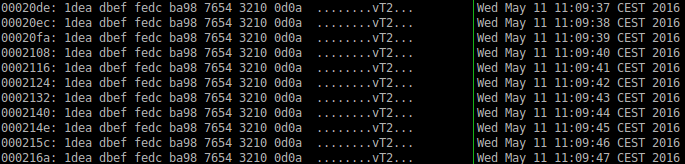
\includegraphics[width=1\textwidth]{graphics/xdd_can_test.png}
  \label{fig:boat1}
  \caption{Left shows output from command \ref{code:xxd} and right shows command \ref{code:bash_send_can}}
\end{figure}
It can be seen that the received ID and data is \textit{1deadbef} and \textit{fedcba9876543210} respectively.\\
\textit{0d0a} is \textbackslash r and \textbackslash n respectively.



\newpage
%\subsection{Tasks}
%\input{tasks}
%\newpage

%\subsection{Wireless communication}
%\subsubsection*{Communication flow}
\input{communication_flow}
bstract.tex


\newpage



\newpage
\section{AutoQuad M4 firmware} \label{sec:aq_m4_firmware}
\textbf{AutoQuad} is the flight controller used in this project. The author was among the first students using AutoQuad on SDU, but the first student to make changes to the firmware and to communicate with AQ using CAN-bus. The AutoQuad firmware was not documented at all, so much time was spend reading through code and trying to figure out how it works. A great amount of time was also spend on more practical things like getting to know their Development Environment (CrossWorks for ARM)\footnote{http://www.rowley.co.uk/arm/} in order to compile their firmware, waiting for Quatos\footnote{The controller, Quatos,  used in AutoQuad is not Open Source so a license had to be bought by SDU} license and getting familiar with the flashing process of AutoQuad.\\
Much of the gained knowledge about AutoQuad and how to do debugging has been written down to share with other students. It can be found on the USB-key handed in \textit{Appendix/SDU-UASAutoQuaddocumentation.pdf and SDU-UASAutoQuadsourcecodedocumentation.pdf}. Text marked with green is written by the author.


\textit{Since AutoQuad only supports proving GPS coordinates through a serial port\footnote{Seen by inspection of the schematic to the M4-board done by the supervisor} another way had to be found and implemented.
Sending GPS coordinates through the serial port would require the onboard GPS to be unmounted which seems like a bad solution. The CAN bus was chosen since it is already implemented in AutoQuad. However AutoQuad supports sensor inputs through CAN, GPS was not supported and there by had to be implemented.}

In order to send GPS coordinates to AQ a way in had to be found. A solution would be to unmount the onboard GPS, however that removes the functionality of the M4 board to fly normally without external hardware eg. A RPI. Since AutoQuad gets its coordinates from the onboard ublox M8Q \footnote{\url{http://autoquad.org/wiki/wiki/m4-microcontroller/m4-gps-antenna-options/}} using ublox's ubx protocol, everything sent by eg. a RPI had to be encoded as ubx.
Instead of making hardware changes to the M4 it was decided to use the already supported CAN-bus interface. The M4 board already uses the CAN-bus to send velocities to each of the ESC's on an EduQuad drone. AutoQuad default supports sending some sensor values using the CAN-bus, however GPS coordinates, DOPs and accuracies was not implemented. The only implementation was to receive the battery voltage and current usage and log it to an MicroSD-card.
AutoQuads CAN protocol is described, implemented and tested in section \ref{sec:somewhere}.

When all CAN-nodes has successfully registered, different node-initializing functions run.
First a summary run which sends the number and types of the nodes to QGroundStation. \footnote{Graphical userinterface which provices generel information about the drone such as battery, attitude but also waypoint functionalities}.
It can thus be validated by the pilot that all the ESC's and CAN-sensors are detected.
After the summary, a CAN-sensor initialization happens. The initialization of each CAN-sensor happens which is to send CAN\_CMD\_TELEM\_* described in section \ref{sec:somewhere} but more important also to create a callback.
The callback will then be attached to the CAN-type which in this case is CAN-sensor\footnote{CAN-types are described in section \ref{sec:somewhere}} so when AutoQuad receives a sensor reading the callback will be invoked.\\

Default the callback fills in the sensorvalue in an array so the sensor value can be used in another task. The canID \footnote{Described in section \ref{sec:somewhere}} is then used as index so the task needing the sensorvalue knows where to look since it knows which sensorsvalue it needs. Code \ref{code:callback} shows the callback\footnote{\url{https://github.com/bn999/autoquad/blob/master/onboard/canSensors.c}}
\begin{lstlisting}[language = c, caption = Callback invoked when a CAN-sensorvalue is received. It stores the value in an array indexed by canId, label=code:callback]
void canSensorsReceiveTelem(uint8_t canId, uint8_t doc, void *data) {
    canSensorsData.values[canId] = *(float *)data;

	/* Reception time of the message stored as well */
}
\end{lstlisting}
The callback is fairly simple and does not save the doc\footnote{Described in section \ref{sec:somewhere}} which is needed in order to tell which value the CAN-GPS sensor is sending.\\

All of the CAN-GPS packet handling has been implemented in the callback function. A prettier solution might have been to create a task and use a semaphore to signal when there is a new GPS-packet available. Due to lack of time implementing everything was done in the callback.

Code \ref{code:psudo_parse_can_gps} shows a pseudo code of how the GPS-packets is handled. In section \ref{sec:somewhere} the CAN-GPS packets can be seen.

\begin{lstlisting}[language = Matlab, caption = Modified callback invoked when a sensor-value is received. Shows how doc is used to tell which GPS\-packet is received and when height is received the flags are set, label=code:psudo_parse_can_gps]
canSensorsReceiveTelem(canId, doc, *data) {
	if doc == CAN_DOC_LAT then
		canData.latitude = data
		
	if doc == CAN_DOC_LON then
		canData.longitude = data
		
	if doc == CAN_DOC_DOP then
		canData.xDOP = data[x]
		..
	if doc == CAN_DOC_ACC then
		canData.satellites = data[0]
		canData.fix = data[1]
		canData.xAcc = data[x]
		..
		canData.heading = data[n-1]
		
	if doc == CAN_DOC_VEL then
		gpsData.velx = data[x]
		..		
	if doc == CAN_DOC_ALT then
		gpsDatat.height = data
		if gpsData.fix == 1 and gpsData.satellites >= 8 then
			gpsUpdatetime = now()
			setFlag (gpsData.gpsPosFlag)
			setFlag (gpsData.gpsVelFlag)
		else:
			debug_to_QGroundStation
}
\end{lstlisting}

The \textit{data} pointer given as parameter to the callback is of void pointer. Some pointer gymnastics is done in order to get the right elements from the CAN-packet. If the received CAN-packet is of 8*1 bytes, the void pointer is casted to an uint8\_t pointer so each byte can be retrieved by using the casted pointer as an array. \\

When the flags are set, the task updating the UKF will run \footnote{\url{https://github.com/bn999/autoquad/blob/master/onboard/run.c\#L110} last visited 23 maj}.
Code \ref{code:ukf_update} shows a snippet from the task updating the UKF when the position or velocity flag is set.
\begin{lstlisting}[language = Matlab, caption = Snippet of run.c as psudeocode which updates the UKF when position flag or velocity flag is set, label=code:ukf_update]
if IsFlagSet(gpsData.gpsPosFlag) == yes then
	    navUkfGpsPosUpdate(gpsData.lastPosUpdate, gpsData.lat, gpsData.lon, gpsData.height, ....);
	    ClearFlag(gpsData.gpsPosFlag);
	    
else if IsFlagSet(gpsData.gpsVelFlag) == yes then
	    navUkfGpsVelUpdate(gpsData.lastVelUpdate, gpsData.velN, gpsData.velE, ....);
	    ClearFlag(gpsData.gpsVelFlag);
\end{lstlisting}
bstract.tex


\newpage
\section{Wireless communication}
\subsubsection*{Communication flow}
\begin{table}[H]
\centering

\begin{tabularx}{0.75\textwidth}{@{}|X|X|X|X|X|X|@{}}
\toprule
Content & Lat    & Lon    & Height & DOP   & CRC-16  \\ \midrule
Datatype    & double & double & float  & float & uint16\_t \\ \midrule
Bytes    & 31:24  & 23:16   & 15:8    & 7:4 & 3:0 \\ \bottomrule
\end{tabularx}
\Mathias{Ændre 0:3 til 0:1 da en uint16\_t kun tager 2 bytes og ikke 4}
\caption{Message sent from PC to ESP8266}
\label{my-label}
\end{table}


bstract.tex


\newpage
%\section{Information flow}}
%\textbf{AutoQuad} is the flight controller used in this project. The author was among the first students using AutoQuad on SDU, but the first student to make changes to the firmware and to communicate with AQ using CAN-bus. The AutoQuad firmware was not documented at all, so much time was spend reading through code and trying to figure out how it works. A great amount of time was also spend on more practical things like getting to know their Development Environment (CrossWorks for ARM)\footnote{http://www.rowley.co.uk/arm/} in order to compile their firmware, waiting for Quatos\footnote{The controller, Quatos,  used in AutoQuad is not Open Source so a license had to be bought by SDU} license and getting familiar with the flashing process of AutoQuad.\\
Much of the gained knowledge about AutoQuad and how to do debugging has been written down to share with other students. It can be found on the USB-key handed in \textit{Appendix/SDU-UASAutoQuaddocumentation.pdf and SDU-UASAutoQuadsourcecodedocumentation.pdf}. Text marked with green is written by the author.


\textit{Since AutoQuad only supports proving GPS coordinates through a serial port\footnote{Seen by inspection of the schematic to the M4-board done by the supervisor} another way had to be found and implemented.
Sending GPS coordinates through the serial port would require the onboard GPS to be unmounted which seems like a bad solution. The CAN bus was chosen since it is already implemented in AutoQuad. However AutoQuad supports sensor inputs through CAN, GPS was not supported and there by had to be implemented.}

In order to send GPS coordinates to AQ a way in had to be found. A solution would be to unmount the onboard GPS, however that removes the functionality of the M4 board to fly normally without external hardware eg. A RPI. Since AutoQuad gets its coordinates from the onboard ublox M8Q \footnote{\url{http://autoquad.org/wiki/wiki/m4-microcontroller/m4-gps-antenna-options/}} using ublox's ubx protocol, everything sent by eg. a RPI had to be encoded as ubx.
Instead of making hardware changes to the M4 it was decided to use the already supported CAN-bus interface. The M4 board already uses the CAN-bus to send velocities to each of the ESC's on an EduQuad drone. AutoQuad default supports sending some sensor values using the CAN-bus, however GPS coordinates, DOPs and accuracies was not implemented. The only implementation was to receive the battery voltage and current usage and log it to an MicroSD-card.
AutoQuads CAN protocol is described, implemented and tested in section \ref{sec:somewhere}.

When all CAN-nodes has successfully registered, different node-initializing functions run.
First a summary run which sends the number and types of the nodes to QGroundStation. \footnote{Graphical userinterface which provices generel information about the drone such as battery, attitude but also waypoint functionalities}.
It can thus be validated by the pilot that all the ESC's and CAN-sensors are detected.
After the summary, a CAN-sensor initialization happens. The initialization of each CAN-sensor happens which is to send CAN\_CMD\_TELEM\_* described in section \ref{sec:somewhere} but more important also to create a callback.
The callback will then be attached to the CAN-type which in this case is CAN-sensor\footnote{CAN-types are described in section \ref{sec:somewhere}} so when AutoQuad receives a sensor reading the callback will be invoked.\\

Default the callback fills in the sensorvalue in an array so the sensor value can be used in another task. The canID \footnote{Described in section \ref{sec:somewhere}} is then used as index so the task needing the sensorvalue knows where to look since it knows which sensorsvalue it needs. Code \ref{code:callback} shows the callback\footnote{\url{https://github.com/bn999/autoquad/blob/master/onboard/canSensors.c}}
\begin{lstlisting}[language = c, caption = Callback invoked when a CAN-sensorvalue is received. It stores the value in an array indexed by canId, label=code:callback]
void canSensorsReceiveTelem(uint8_t canId, uint8_t doc, void *data) {
    canSensorsData.values[canId] = *(float *)data;

	/* Reception time of the message stored as well */
}
\end{lstlisting}
The callback is fairly simple and does not save the doc\footnote{Described in section \ref{sec:somewhere}} which is needed in order to tell which value the CAN-GPS sensor is sending.\\

All of the CAN-GPS packet handling has been implemented in the callback function. A prettier solution might have been to create a task and use a semaphore to signal when there is a new GPS-packet available. Due to lack of time implementing everything was done in the callback.

Code \ref{code:psudo_parse_can_gps} shows a pseudo code of how the GPS-packets is handled. In section \ref{sec:somewhere} the CAN-GPS packets can be seen.

\begin{lstlisting}[language = Matlab, caption = Modified callback invoked when a sensor-value is received. Shows how doc is used to tell which GPS\-packet is received and when height is received the flags are set, label=code:psudo_parse_can_gps]
canSensorsReceiveTelem(canId, doc, *data) {
	if doc == CAN_DOC_LAT then
		canData.latitude = data
		
	if doc == CAN_DOC_LON then
		canData.longitude = data
		
	if doc == CAN_DOC_DOP then
		canData.xDOP = data[x]
		..
	if doc == CAN_DOC_ACC then
		canData.satellites = data[0]
		canData.fix = data[1]
		canData.xAcc = data[x]
		..
		canData.heading = data[n-1]
		
	if doc == CAN_DOC_VEL then
		gpsData.velx = data[x]
		..		
	if doc == CAN_DOC_ALT then
		gpsDatat.height = data
		if gpsData.fix == 1 and gpsData.satellites >= 8 then
			gpsUpdatetime = now()
			setFlag (gpsData.gpsPosFlag)
			setFlag (gpsData.gpsVelFlag)
		else:
			debug_to_QGroundStation
}
\end{lstlisting}

The \textit{data} pointer given as parameter to the callback is of void pointer. Some pointer gymnastics is done in order to get the right elements from the CAN-packet. If the received CAN-packet is of 8*1 bytes, the void pointer is casted to an uint8\_t pointer so each byte can be retrieved by using the casted pointer as an array. \\

When the flags are set, the task updating the UKF will run \footnote{\url{https://github.com/bn999/autoquad/blob/master/onboard/run.c\#L110} last visited 23 maj}.
Code \ref{code:ukf_update} shows a snippet from the task updating the UKF when the position or velocity flag is set.
\begin{lstlisting}[language = Matlab, caption = Snippet of run.c as psudeocode which updates the UKF when position flag or velocity flag is set, label=code:ukf_update]
if IsFlagSet(gpsData.gpsPosFlag) == yes then
	    navUkfGpsPosUpdate(gpsData.lastPosUpdate, gpsData.lat, gpsData.lon, gpsData.height, ....);
	    ClearFlag(gpsData.gpsPosFlag);
	    
else if IsFlagSet(gpsData.gpsVelFlag) == yes then
	    navUkfGpsVelUpdate(gpsData.lastVelUpdate, gpsData.velN, gpsData.velE, ....);
	    ClearFlag(gpsData.gpsVelFlag);
\end{lstlisting}
bstract.tex




seq tæller op så rate/value bliver acknowledged
  can0  00000000   [0] 
  can0  01C00000   [8]  EF BE AD DE 03 09 00 00
  can0  0E000041   [6]  EF BE AD DE 00 00
  can0  14CD0042   [2]  00 08
  can0  00400002   [8]  00 00 00 00 00 00 00 00
  can0  14CC0043   [2]  0A 00
  can0  00400003   [8]  00 00 00 00 00 00 00 00



\section{Indoor localization} \label{sec:indoor_localization}
\textit{In order to do indoor flying there is a need of some sort of localization since GPS is not available. Vision was decided based on what mostly others are using and some further advantages. Instead of making the vision, it is decided to use an existing tracker called MarkerLocator written by Henrik Midtiby. However the MarkerLocator lacks a proper quality measure so that is implemented. A few tests were made and the MarkerLocator with implemented quality measure suits the needs in this project.}


In order to do accurate flying indoor a localization system is needed. In the Related Work section, it can be seen vision with a camera mounted pointing down is used by others. Compared to use one or more cameras mounted on the drone, an advantage of using a camera mounted on the ceiling is that the camera will not be harmed if the drone crashes and that one camera can be used to detect several drones. However if the position is needed in more than 2D, more than one camera might be needed(depending on the algorithm used) but it still scales better than mounting one or more cameras on each drone. \\

Based on previous experience, the MarkerLocator written by Henrik Midtiby was chosen as indoor localization. Its using OpenCV\footnote{\url{http://opencv.org/}} and implemented in python. It works by detecting markers as shown in figure \ref{fig:markerlocator_marker}
\Mathias{insert image of markerLocator marker with different orders}


\begin{figure}[H]
    \centering
    \begin{subfigure}[b]{0.2\textwidth}
        
\includegraphics[width=\textwidth]{graphics/marker_order_4.pdf}
        \caption{Marker of order 4 used to get the 2D position of a drone}
        \label{fig:markerlocator_order_4}
    \end{subfigure}
    \quad %add desired spacing between images, e. g. ~, \quad, \qquad, \hfill etc. 
      %(or a blank line to force the subfigure onto a new line)
    \begin{subfigure}[b]{0.2\textwidth}
        
\includegraphics[width=\textwidth]{graphics/marker_order_6.pdf}
        \caption{Marker of order 6 used to get the 2D position of a drone}
        \label{fig:markerlocator_order_4}
    \end{subfigure}
    \caption{The markers have one arm less than the order of the marker for the MarkerLocator to detect the orientation of the marker}\label{fig:markerlocator_marker}
\end{figure}




The MarkerLocator works by making a convolution sum of a complex kernel on each frame obtained from the camera.
The location where if fits best is said to be the location of the marker in the frame.
How it works in detail is out the scope of this project.
The markers shown in figure \ref{fig:markerlocator_marker} is of different orders.
The order is equal to the number of black arms minus one since the missing arm is used to detect the orientation of the marker. 
Different orders can be used and thereby detect more than one marker in each frame. Unfortunately it can only get the 2D position and 1D orientation of the marker.
Since doing a convolution of the entire frame is relatively slow \footnote{Processing one fullHD frame takes approximately 0.38 sec. Measured with build in timer in the MarkerLocator}, the MarkerLocator has a mode called WindowMode.
It works by searching in only a small area around the last known position of the marker and thereby speeding up the progress\footnote{Approximately 0.0041 sec}. 

\begin{figure}[H]
    \center
    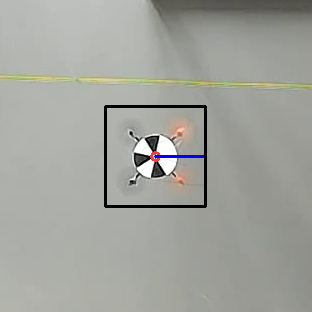
\includegraphics[width=0.4\textwidth]{graphics/markerlocator_window.png}
  	\caption{The MarkerLocator searches only for the marker around the last known position of the marker in a frame of 100*100px.}
    \label{markerlocator_windowmode}
\end{figure}
If the marker moves out of the window, the MarkerLocator is still looking in only that window.
Therefore it is important to have a quality measure that can be used to decide whenever a full convolution of the frame has to be done or if the marker has been found within the window. 

The MarkerLocator has a quality measure build-in used to tell how well the marker is detected. However it is not used in the MarkerLocator to tell if a full convolution has to be done. 
The quality measure implemented in the MarkerLocator is a hack \footnote{Said by Henrik Midtiby} and is known from previous applications that it is a bad measure of the right marker is detected.

In cooperation with Henrik Midtiby a few quality measures was developed. The overall idea was to compare the kernel used to do the convolution with the marker found in the frame.
Different algorithms where used to give a normalized value telling how similar the found marker is to the kernel. Figure \ref{fig:markerlocator_algorithms} shows the different solutions tried.\\

\begin{figure}[H]
    \centering
    \begin{subfigure}[b]{0.3\textwidth}
        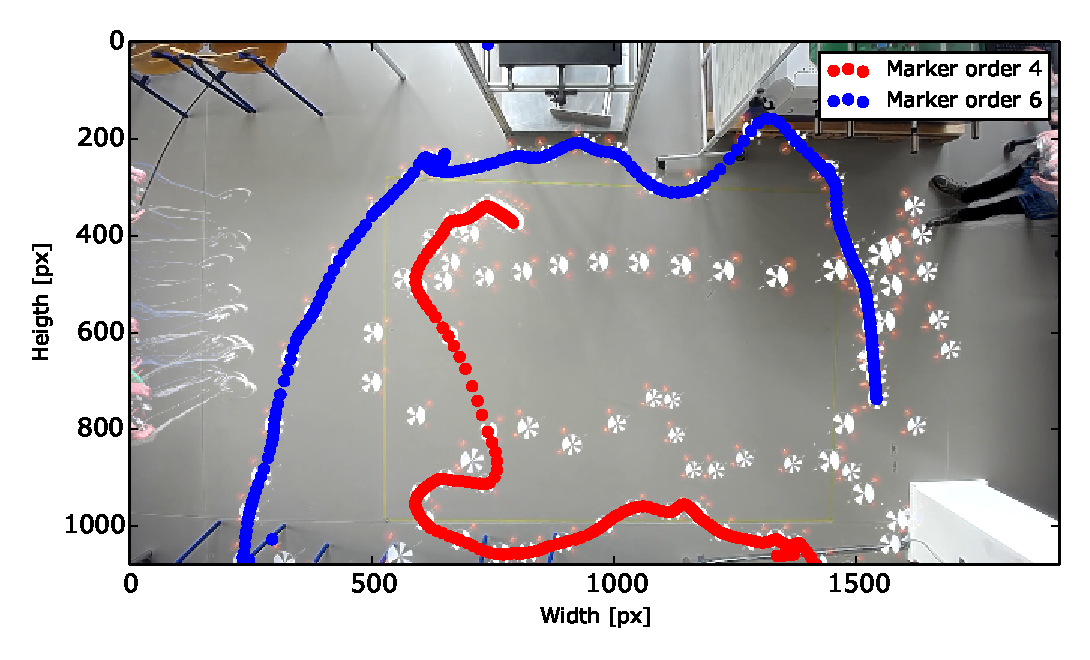
\includegraphics[width=\textwidth]{graphics/markerlocator_compare_raw.eps}
        \caption{Counting pixel match suffers from being unable to find the markers if lost}
        \label{fig:markerlocator_algorihm_native}
    \end{subfigure}
    ~ %add desired spacing between images, e. g. ~, \quad, \qquad, \hfill etc. 
      %(or a blank line to force the subfigure onto a new line)
    \begin{subfigure}[b]{0.3\textwidth}
        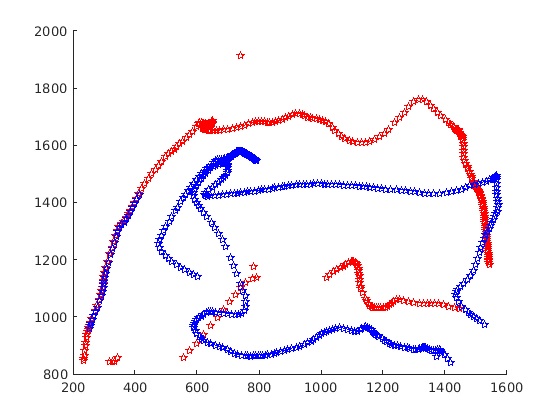
\includegraphics[width=\textwidth]{graphics/markerlocator_ssim.png}
        \caption{SSIM suffers from false positives and a few false negative}
        \label{fig:markerlocator_algorithm_ssim}
    \end{subfigure}
    ~
    \begin{subfigure}[b]{0.3\textwidth}
        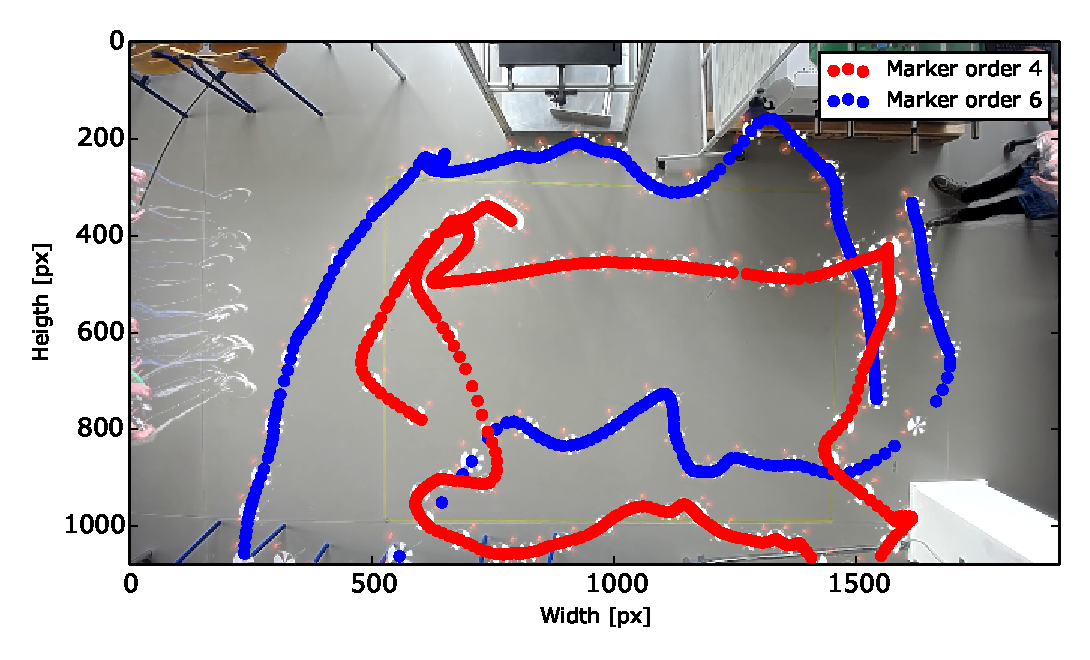
\includegraphics[width=\textwidth]{graphics/markerlocator_match_order.eps}
        \caption{Developed algorithm has no false negative of positive and is able to find the markers if lost}
        \label{fig:markerlocator_algorithm_order_match}
    \end{subfigure}
    \caption{Different approaches to get a quality measure explaining how well the right marker is found.}\label{fig:markerlocator_algorithms}
\end{figure}

Figure \ref{fig:markerlocator_algorihm_native} is a native approach of comparing all pixels in the kernel with the pixels in the found marker. A counter is incremented upon each match and at the end divided by the number of pixels compared in to normalize. A threshold determines weather a marker is found and the next scan should be done in the window of if a full scan is required. The best result is obtained using a threshold of 0.4. If the threshold were lowered false positives started to occur. \\

Figure \ref{fig:markerlocator_algorithm_ssim} uses an algorithm developed to compare similarities in images. 
The details of this algorithm is out of scope the details of this project. The implementation in scipy-image\footnote{\url{http://scikit-image.org/}} was used.
It can seen it performs better than the native approach but a lot of false positive and a few false negative exists. It also suffers from not detecting the markers compared to the native approach. A threshold of 0.3 were used. If the threshold were increased, it would detect less markers. \\

Figure \ref{fig:markerlocator_algorithm_order_match} shows a simple algorithm the author came up with.
If the MarkerLocator is looking for a marker of order 4 and it has detected a marker and its orientation, the algorithm calculates where the location of the arms. It then checks a pixel in each arm and increments a counter if the pixel is black. When it has checked all the arms it compares the counter with the order the MarkerLocator is looking for and returns if they match or not. 
This method does not provide a scalar as output but a binary and thereby has no threshold. However in order to detect if a pixel is black or not, a threshold has been used. The threshold was set to 100 which has shown good results doing tests and flight. \\

During development of quality measures it was noted that if the MarkerLocator does a full search because it cannot find a marker with order 4, it slows down the detection of the marker of order 6. This is because the MarkerLocator is implemented in one process without threading. However this has been solved by splitting up the MarkerLocator in 2 different processes so they run independently of each other. More about this in section  \ref{sec:pc_design} \\

\textbf{Perspective correction} \\
In order to use centimeters as measure of the position of the markers and to correct if the camera is not pointing directly down, the build-in perspective correction in the MarkerLocator were used.
It works by using homography\footcite{janeriksolem2012} to make the transformation from pixels to some chosen unit which in this case is centimeters.
\begin{wrapfigure}{r}{0.5\textwidth}
  \vspace{-20pt}
  \begin{center}
    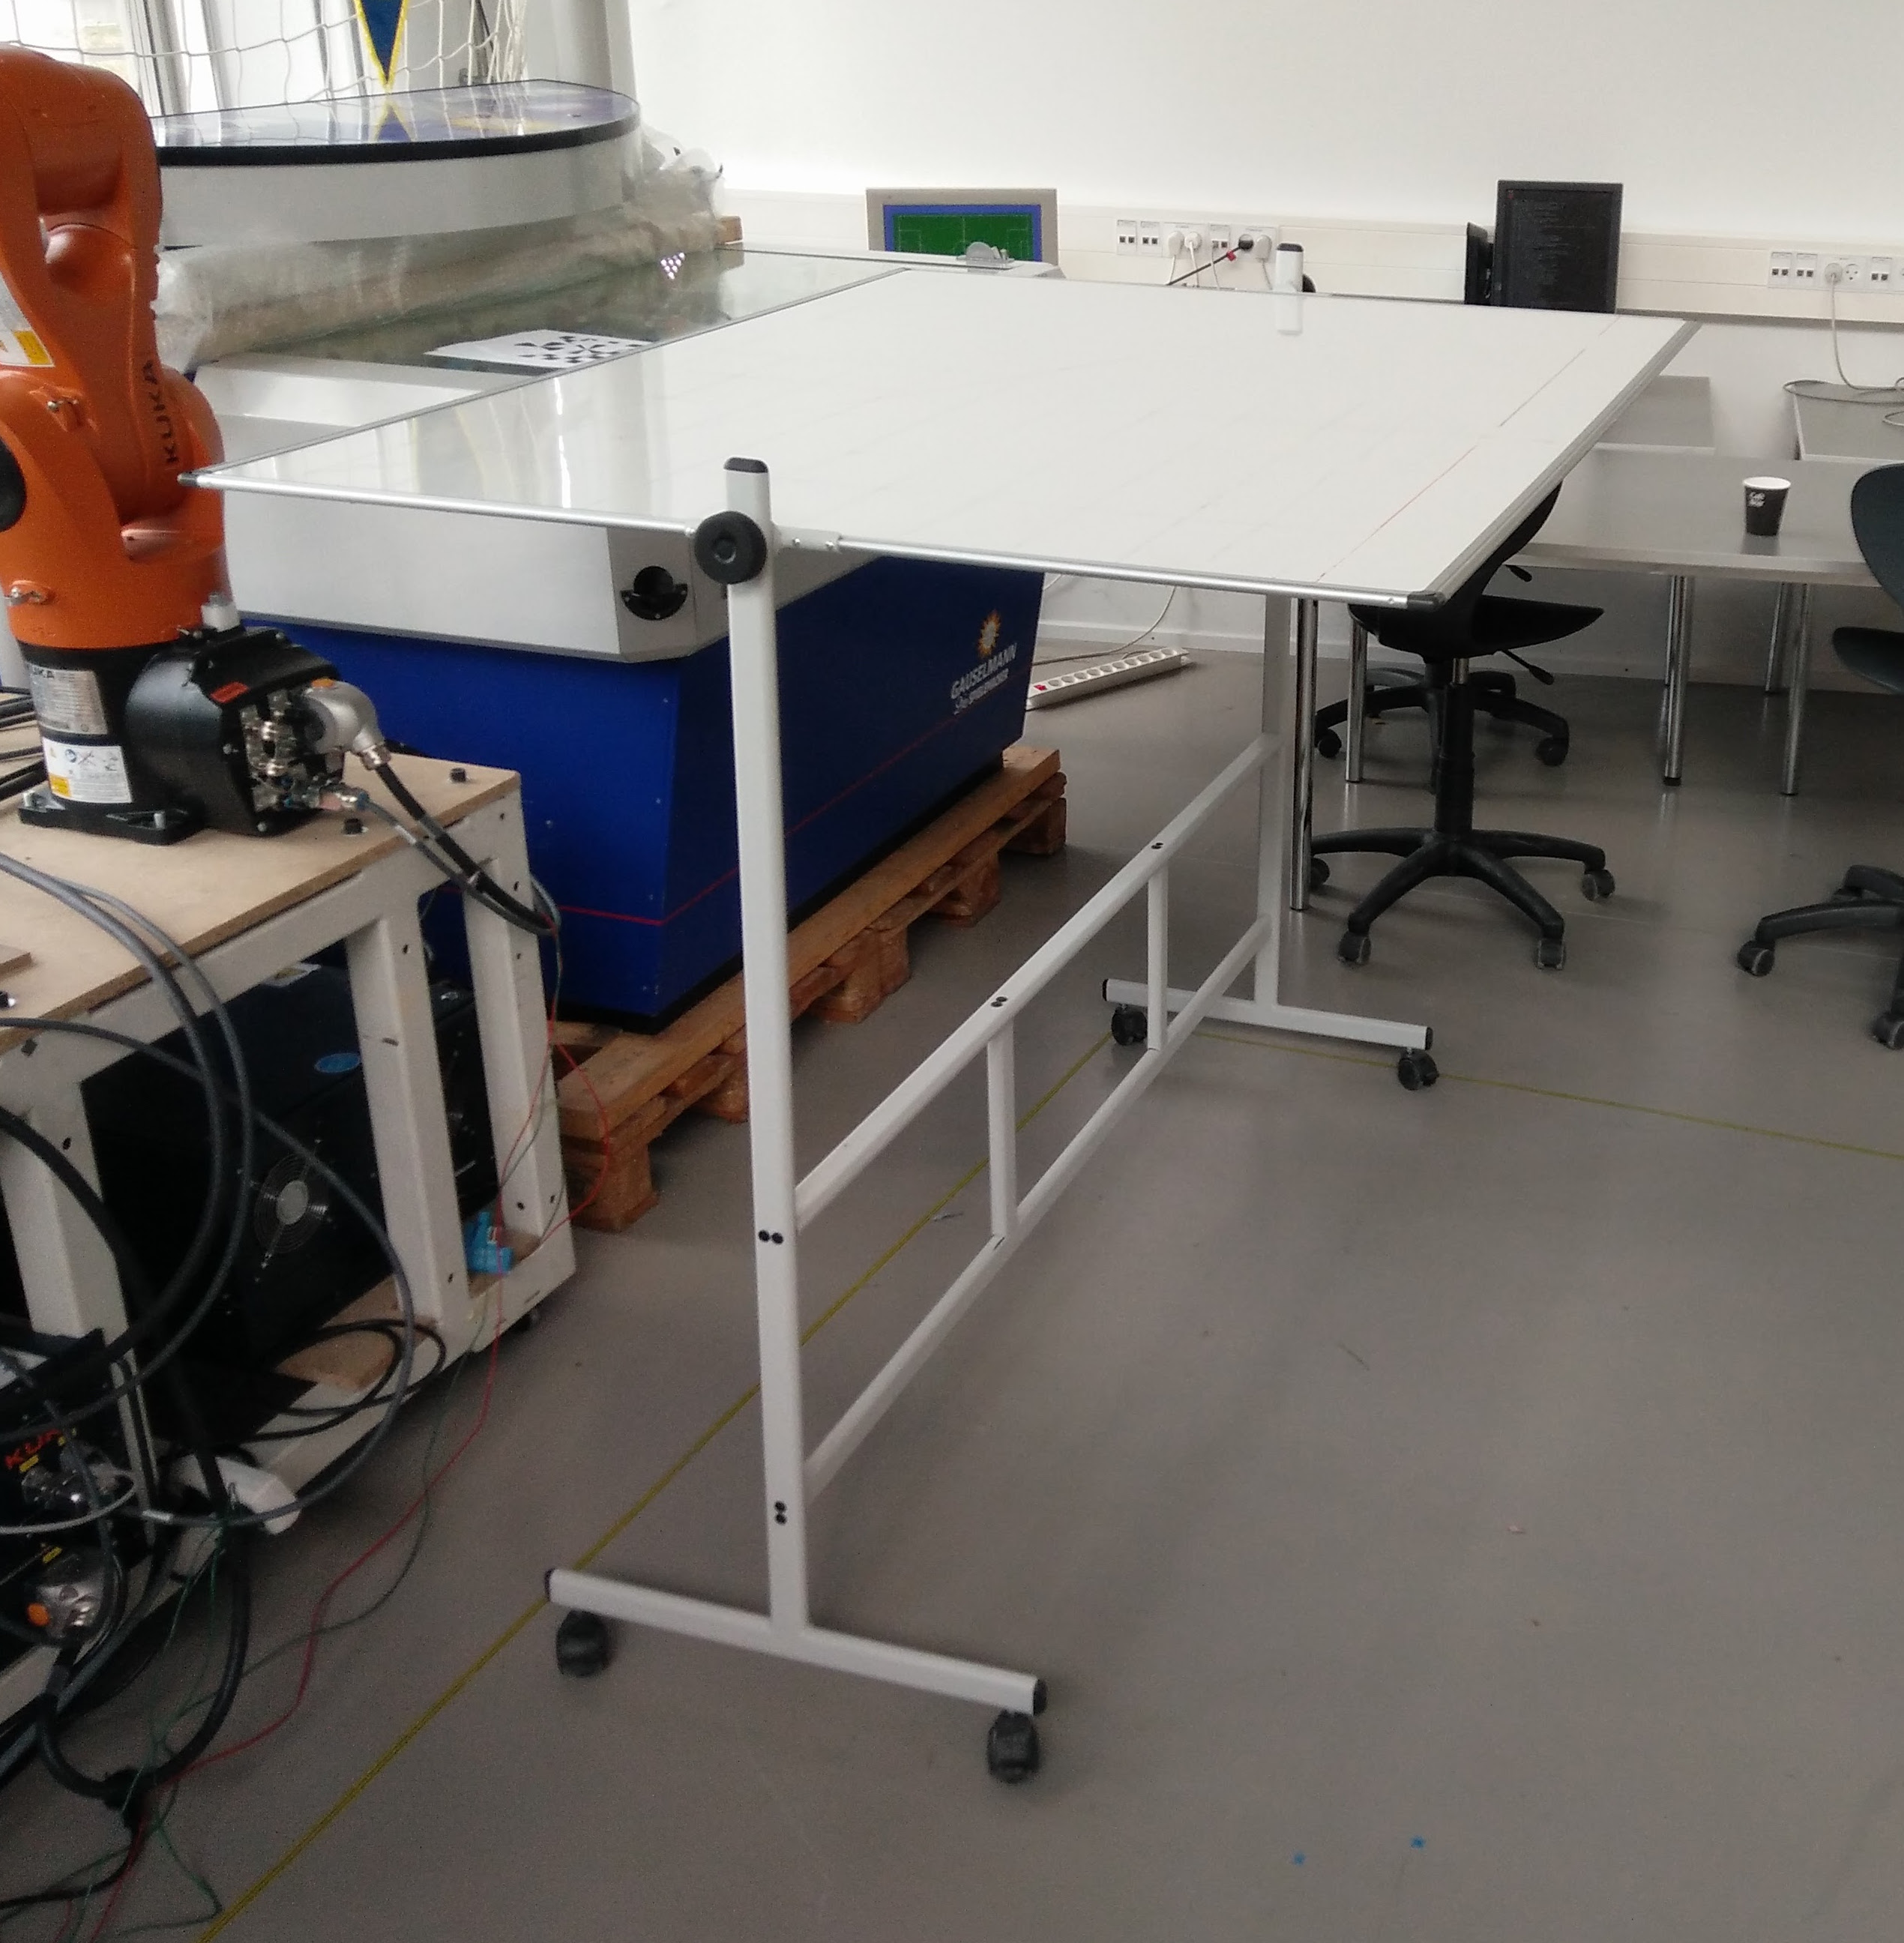
\includegraphics[width=0.48\textwidth]{graphics/whiteboard_tilted.jpg}
  \end{center}
  \vspace{-20pt}
  \caption{Setup used to make 4 points in the flight-height. The four corners of the whiteboard was used and then found in the image. } \label{fig:whiteboard_setup}
  \vspace{-10pt}
\end{wrapfigure}

By creating four markers with known distance to each other at the expected flight height \footnote{Since only 2D positioning is available, a plane where the drone is expected to fly is decided} and find these markers in the frame, it is possible for the perspective corrector to make the transformation.
Figure \ref{fig:whiteboard_setup} shows the setup used. A picture was taken from the ceiling-camera and the four black corners of the whiteboard could be found in the frame. The distance between the black corners in centimeters and the distance in px is given as input to the perspective correcter. The locations of markers is then transformed into the plane made by the whiteboard.


A test was conducted to get the accuracy of the MarkerLocator. Two markers with order 4 and 6 was placed at the expected flight-height and the distance between the two markers was calculated using Pythagoras.\\
The real distance measured by a ruler was 60 cm and and the MarkerLocator gave 59.19 which is an error of 0.81 cm.

Another test was conducted in order to see how stable the MarkerLocator is. 547 position detections was done while the marker was placed steady at the flight height. It shows a mean position in x of -8.1487 with variance of 0, y position with mean -39.5046 and variance 0. \\


It can be concluded that using the MarkerLocator with the improved order detection it is possible to detect two drones without having any false positive/negative. By making a test of the distance between two markers there is an error of 0.81 cm. The MarkerLocator seems stable with a variance of zero. 


\section{Control and coordinate conversion}
\label{sec:control_and_coordinate_conversion}
%\textit{In order to do indoor flying there is a need of some sort of localization since GPS is not available. Vision was decided based on what mostly others are using and some further advantages. Instead of making the vision, it is decided to use an existing tracker called MarkerLocator written by Henrik Midtiby. However the MarkerLocator lacks a proper quality measure so that is implemented. A few tests were made and the MarkerLocator with implemented quality measure suits the needs in this project.}


In order to do accurate flying indoor a localization system is needed. In the Related Work section, it can be seen vision with a camera mounted pointing down is used by others. Compared to use one or more cameras mounted on the drone, an advantage of using a camera mounted on the ceiling is that the camera will not be harmed if the drone crashes and that one camera can be used to detect several drones. However if the position is needed in more than 2D, more than one camera might be needed(depending on the algorithm used) but it still scales better than mounting one or more cameras on each drone. \\

Based on previous experience, the MarkerLocator written by Henrik Midtiby was chosen as indoor localization. Its using OpenCV\footnote{\url{http://opencv.org/}} and implemented in python. It works by detecting markers as shown in figure \ref{fig:markerlocator_marker}
\Mathias{insert image of markerLocator marker with different orders}


\begin{figure}[H]
    \centering
    \begin{subfigure}[b]{0.2\textwidth}
        
\includegraphics[width=\textwidth]{graphics/marker_order_4.pdf}
        \caption{Marker of order 4 used to get the 2D position of a drone}
        \label{fig:markerlocator_order_4}
    \end{subfigure}
    \quad %add desired spacing between images, e. g. ~, \quad, \qquad, \hfill etc. 
      %(or a blank line to force the subfigure onto a new line)
    \begin{subfigure}[b]{0.2\textwidth}
        
\includegraphics[width=\textwidth]{graphics/marker_order_6.pdf}
        \caption{Marker of order 6 used to get the 2D position of a drone}
        \label{fig:markerlocator_order_4}
    \end{subfigure}
    \caption{The markers have one arm less than the order of the marker for the MarkerLocator to detect the orientation of the marker}\label{fig:markerlocator_marker}
\end{figure}




The MarkerLocator works by making a convolution sum of a complex kernel on each frame obtained from the camera.
The location where if fits best is said to be the location of the marker in the frame.
How it works in detail is out the scope of this project.
The markers shown in figure \ref{fig:markerlocator_marker} is of different orders.
The order is equal to the number of black arms minus one since the missing arm is used to detect the orientation of the marker. 
Different orders can be used and thereby detect more than one marker in each frame. Unfortunately it can only get the 2D position and 1D orientation of the marker.
Since doing a convolution of the entire frame is relatively slow \footnote{Processing one fullHD frame takes approximately 0.38 sec. Measured with build in timer in the MarkerLocator}, the MarkerLocator has a mode called WindowMode.
It works by searching in only a small area around the last known position of the marker and thereby speeding up the progress\footnote{Approximately 0.0041 sec}. 

\begin{figure}[H]
    \center
    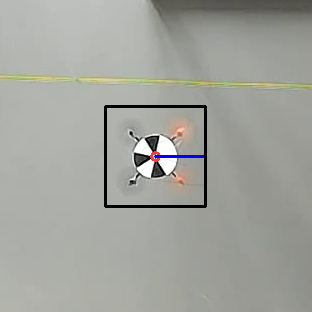
\includegraphics[width=0.4\textwidth]{graphics/markerlocator_window.png}
  	\caption{The MarkerLocator searches only for the marker around the last known position of the marker in a frame of 100*100px.}
    \label{markerlocator_windowmode}
\end{figure}
If the marker moves out of the window, the MarkerLocator is still looking in only that window.
Therefore it is important to have a quality measure that can be used to decide whenever a full convolution of the frame has to be done or if the marker has been found within the window. 

The MarkerLocator has a quality measure build-in used to tell how well the marker is detected. However it is not used in the MarkerLocator to tell if a full convolution has to be done. 
The quality measure implemented in the MarkerLocator is a hack \footnote{Said by Henrik Midtiby} and is known from previous applications that it is a bad measure of the right marker is detected.

In cooperation with Henrik Midtiby a few quality measures was developed. The overall idea was to compare the kernel used to do the convolution with the marker found in the frame.
Different algorithms where used to give a normalized value telling how similar the found marker is to the kernel. Figure \ref{fig:markerlocator_algorithms} shows the different solutions tried.\\

\begin{figure}[H]
    \centering
    \begin{subfigure}[b]{0.3\textwidth}
        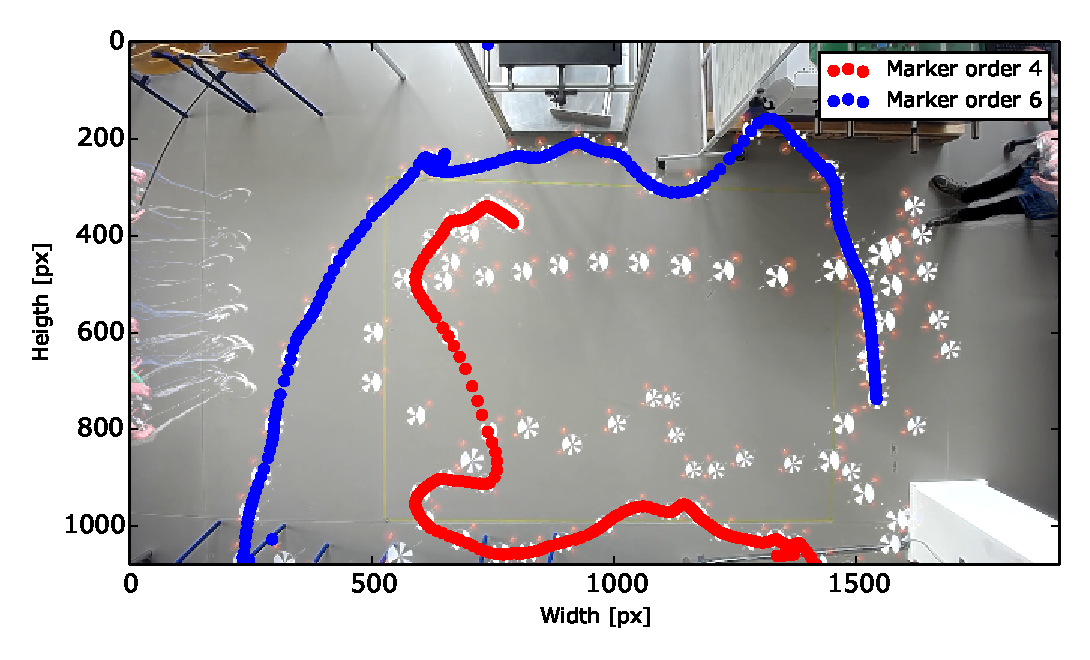
\includegraphics[width=\textwidth]{graphics/markerlocator_compare_raw.eps}
        \caption{Counting pixel match suffers from being unable to find the markers if lost}
        \label{fig:markerlocator_algorihm_native}
    \end{subfigure}
    ~ %add desired spacing between images, e. g. ~, \quad, \qquad, \hfill etc. 
      %(or a blank line to force the subfigure onto a new line)
    \begin{subfigure}[b]{0.3\textwidth}
        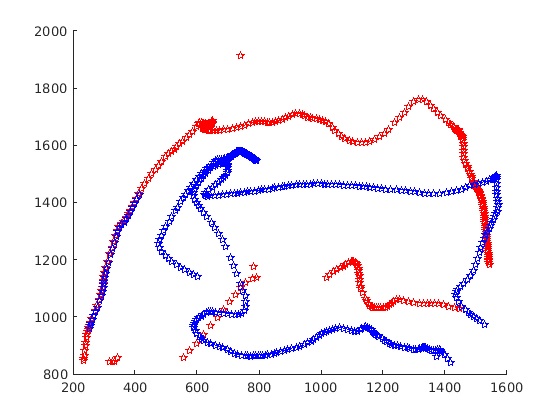
\includegraphics[width=\textwidth]{graphics/markerlocator_ssim.png}
        \caption{SSIM suffers from false positives and a few false negative}
        \label{fig:markerlocator_algorithm_ssim}
    \end{subfigure}
    ~
    \begin{subfigure}[b]{0.3\textwidth}
        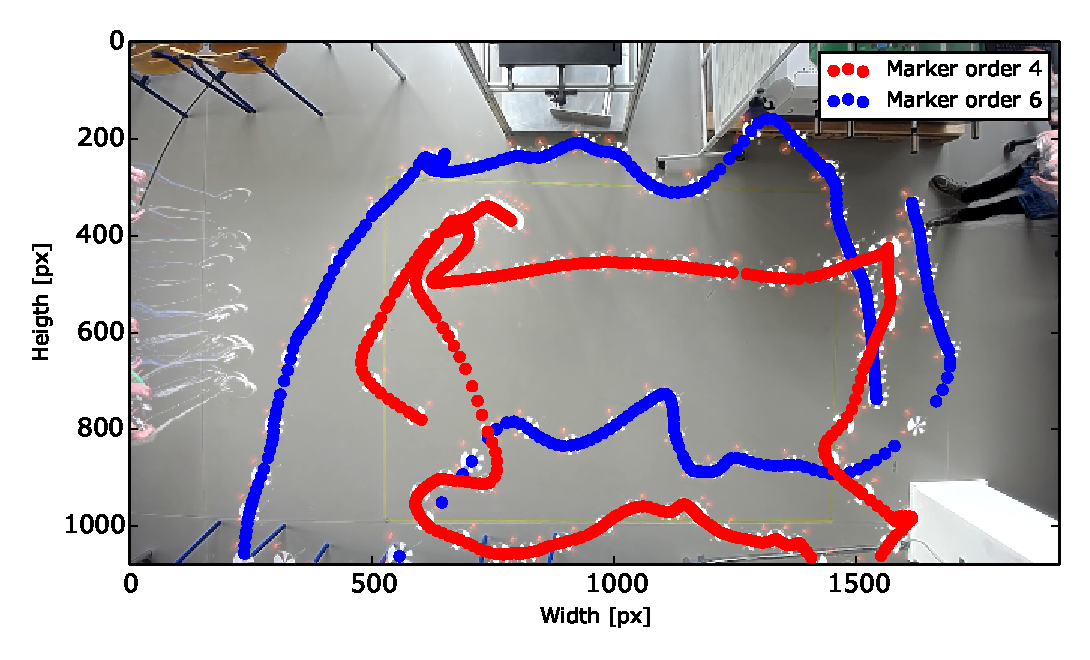
\includegraphics[width=\textwidth]{graphics/markerlocator_match_order.eps}
        \caption{Developed algorithm has no false negative of positive and is able to find the markers if lost}
        \label{fig:markerlocator_algorithm_order_match}
    \end{subfigure}
    \caption{Different approaches to get a quality measure explaining how well the right marker is found.}\label{fig:markerlocator_algorithms}
\end{figure}

Figure \ref{fig:markerlocator_algorihm_native} is a native approach of comparing all pixels in the kernel with the pixels in the found marker. A counter is incremented upon each match and at the end divided by the number of pixels compared in to normalize. A threshold determines weather a marker is found and the next scan should be done in the window of if a full scan is required. The best result is obtained using a threshold of 0.4. If the threshold were lowered false positives started to occur. \\

Figure \ref{fig:markerlocator_algorithm_ssim} uses an algorithm developed to compare similarities in images. 
The details of this algorithm is out of scope the details of this project. The implementation in scipy-image\footnote{\url{http://scikit-image.org/}} was used.
It can seen it performs better than the native approach but a lot of false positive and a few false negative exists. It also suffers from not detecting the markers compared to the native approach. A threshold of 0.3 were used. If the threshold were increased, it would detect less markers. \\

Figure \ref{fig:markerlocator_algorithm_order_match} shows a simple algorithm the author came up with.
If the MarkerLocator is looking for a marker of order 4 and it has detected a marker and its orientation, the algorithm calculates where the location of the arms. It then checks a pixel in each arm and increments a counter if the pixel is black. When it has checked all the arms it compares the counter with the order the MarkerLocator is looking for and returns if they match or not. 
This method does not provide a scalar as output but a binary and thereby has no threshold. However in order to detect if a pixel is black or not, a threshold has been used. The threshold was set to 100 which has shown good results doing tests and flight. \\

During development of quality measures it was noted that if the MarkerLocator does a full search because it cannot find a marker with order 4, it slows down the detection of the marker of order 6. This is because the MarkerLocator is implemented in one process without threading. However this has been solved by splitting up the MarkerLocator in 2 different processes so they run independently of each other. More about this in section  \ref{sec:pc_design} \\

\textbf{Perspective correction} \\
In order to use centimeters as measure of the position of the markers and to correct if the camera is not pointing directly down, the build-in perspective correction in the MarkerLocator were used.
It works by using homography\footcite{janeriksolem2012} to make the transformation from pixels to some chosen unit which in this case is centimeters.
\begin{wrapfigure}{r}{0.5\textwidth}
  \vspace{-20pt}
  \begin{center}
    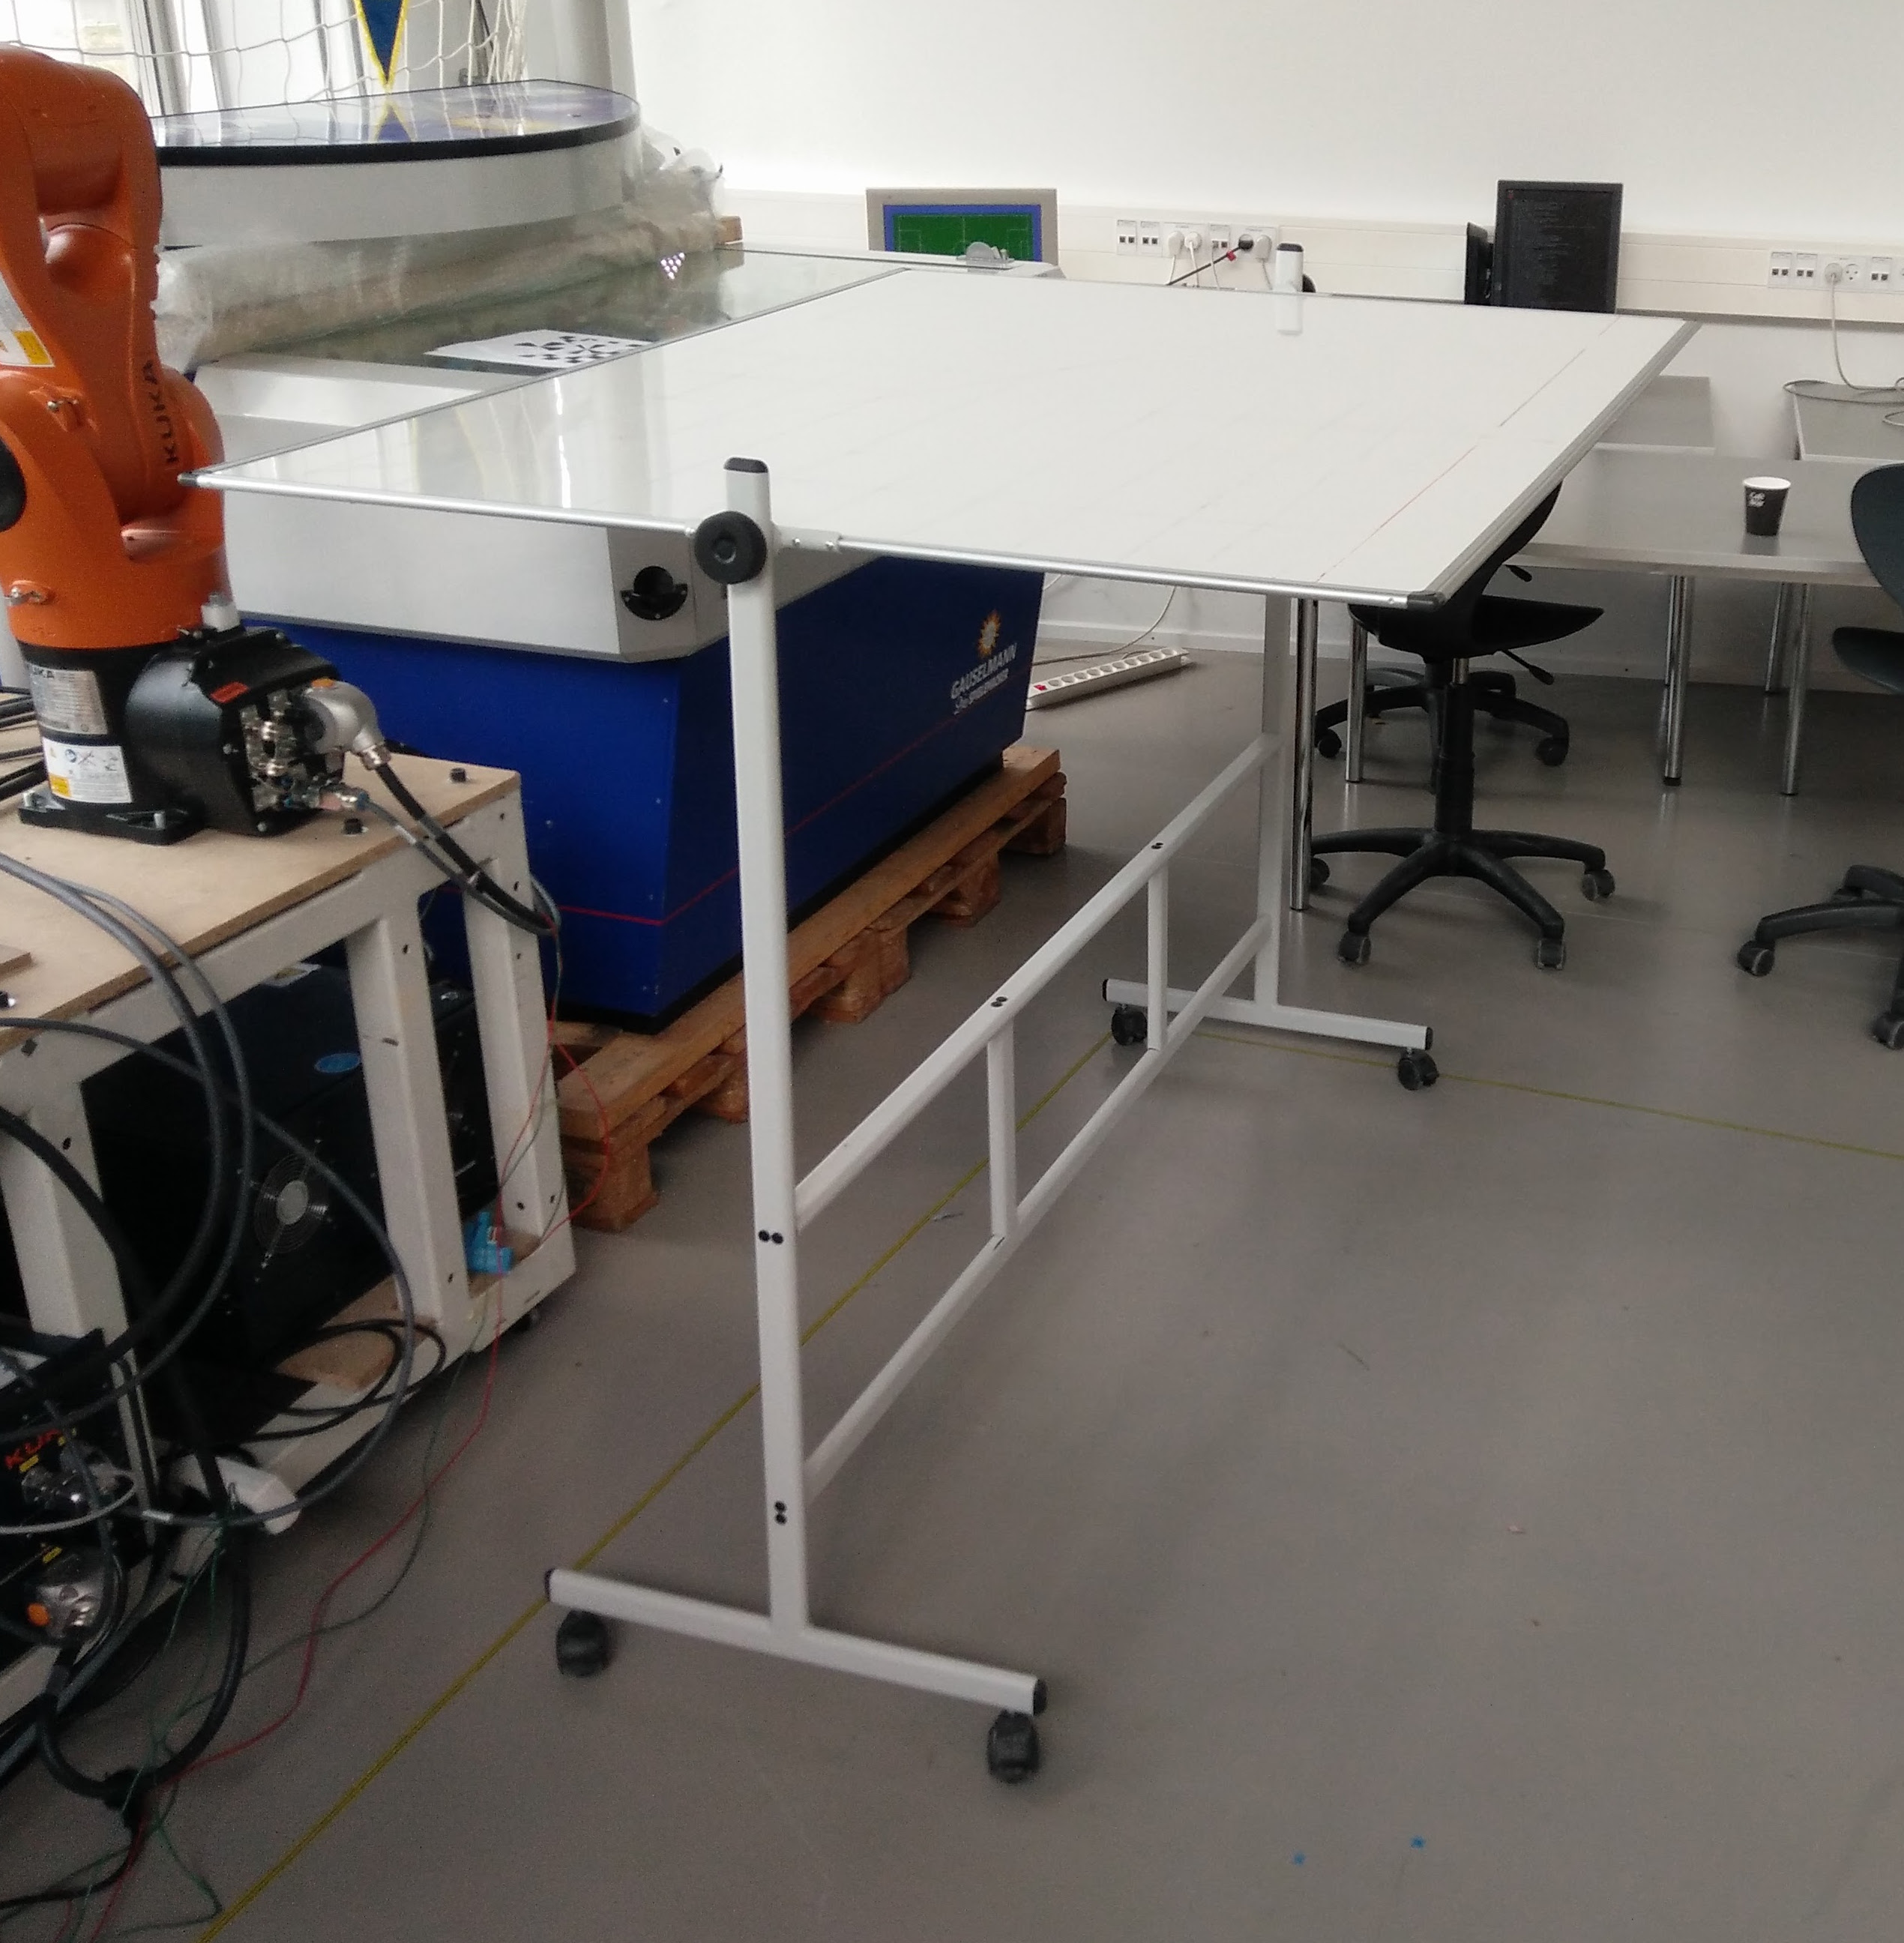
\includegraphics[width=0.48\textwidth]{graphics/whiteboard_tilted.jpg}
  \end{center}
  \vspace{-20pt}
  \caption{Setup used to make 4 points in the flight-height. The four corners of the whiteboard was used and then found in the image. } \label{fig:whiteboard_setup}
  \vspace{-10pt}
\end{wrapfigure}

By creating four markers with known distance to each other at the expected flight height \footnote{Since only 2D positioning is available, a plane where the drone is expected to fly is decided} and find these markers in the frame, it is possible for the perspective corrector to make the transformation.
Figure \ref{fig:whiteboard_setup} shows the setup used. A picture was taken from the ceiling-camera and the four black corners of the whiteboard could be found in the frame. The distance between the black corners in centimeters and the distance in px is given as input to the perspective correcter. The locations of markers is then transformed into the plane made by the whiteboard.


A test was conducted to get the accuracy of the MarkerLocator. Two markers with order 4 and 6 was placed at the expected flight-height and the distance between the two markers was calculated using Pythagoras.\\
The real distance measured by a ruler was 60 cm and and the MarkerLocator gave 59.19 which is an error of 0.81 cm.

Another test was conducted in order to see how stable the MarkerLocator is. 547 position detections was done while the marker was placed steady at the flight height. It shows a mean position in x of -8.1487 with variance of 0, y position with mean -39.5046 and variance 0. \\


It can be concluded that using the MarkerLocator with the improved order detection it is possible to detect two drones without having any false positive/negative. By making a test of the distance between two markers there is an error of 0.81 cm. The MarkerLocator seems stable with a variance of zero. 




%\chapter{Test descriptions} \label{chp:test_descriptions}
%\textit{The following tests were made in order to verify the individual parts was working as expected}


\section{WIFI latency and range} \label{sec:test_wifi_range_ping}
A purpose of the test was to see how the latency and range behaves when the distance is increased.
The firmware of the ESP8266 module had to be flashed to specify which access point \footnote{The network configuration is described in section \ref{sec:network_configuration}} it should connect to.
The test was conducted by increasing the distance between the ESP8266 module and the laptop by 1 meter. After each distance increase, the laptop pinged the ESP8266 module 200 times with 10 hz with a packet size equal to the size of the frame used.\footnote{The WIFI frame is described in section \ref{sec:system_architecture_indoor}}. 
The tests were conducted on an open grass field in order to avoid as much disturbance as possible.


\section{WIFI range with CRC} \label{sec:test_wifi_range_crc}
The purpose of a second test was to see what happens with the number of valid CRC\footnote{CRC described in section \ref{sec:extension_board_firmware}} frames\footnote{Frame described in section \ref{sec:system_architecture_indoor}} as the distance is increased.
The distance was increased by 1 meter in the beginning, however to save to it was increased to 5 meters and later 10 meters. However then the module started to miss frames or CRC was not verified the distance between tests went down to 5 meter again.


\section{WIFI with two extension-boards}
The purpose of this test was to see if two ESP8266 modules can receive frames from a laptop at 10 hz, 200 times at a distance of 10 meters when they are receiving at the same time.
Unfortunately only one connector to communicate with the extension-board were made which made it difficult to check if both extension-boards received the data without error at the same time. The test was done 4 times while alternating between the modules to verify both modules were receiving all the packets.\footnote{If more time were available, a timing-test of the setup would have been done. By measuring the time it takes one drones to receive 200 packets, do the same test but when two drones each receiving 200 packets.}

\begin{figure}[H]
    \centering
        \includegraphics[width=0.5\textwidth]{graphics/laptop_extenbioard_crc_check}
        \caption{Test setup where two modules receives 200 frames at 10 hz at the same time. It can be seen that the laptop only checks the received number of frames one extension-board at a time.}
        \label{fig:wifi_two_modules_check}
\end{figure}

%\chapter{Results}\label{chp:results}
%\section{WIFI latency and range} \label{sec:result_wifi_range_ping}
Figure \ref{fig:wifi_pingtest} shows the results of the ping test.

\begin{figure}[H]
    \center
    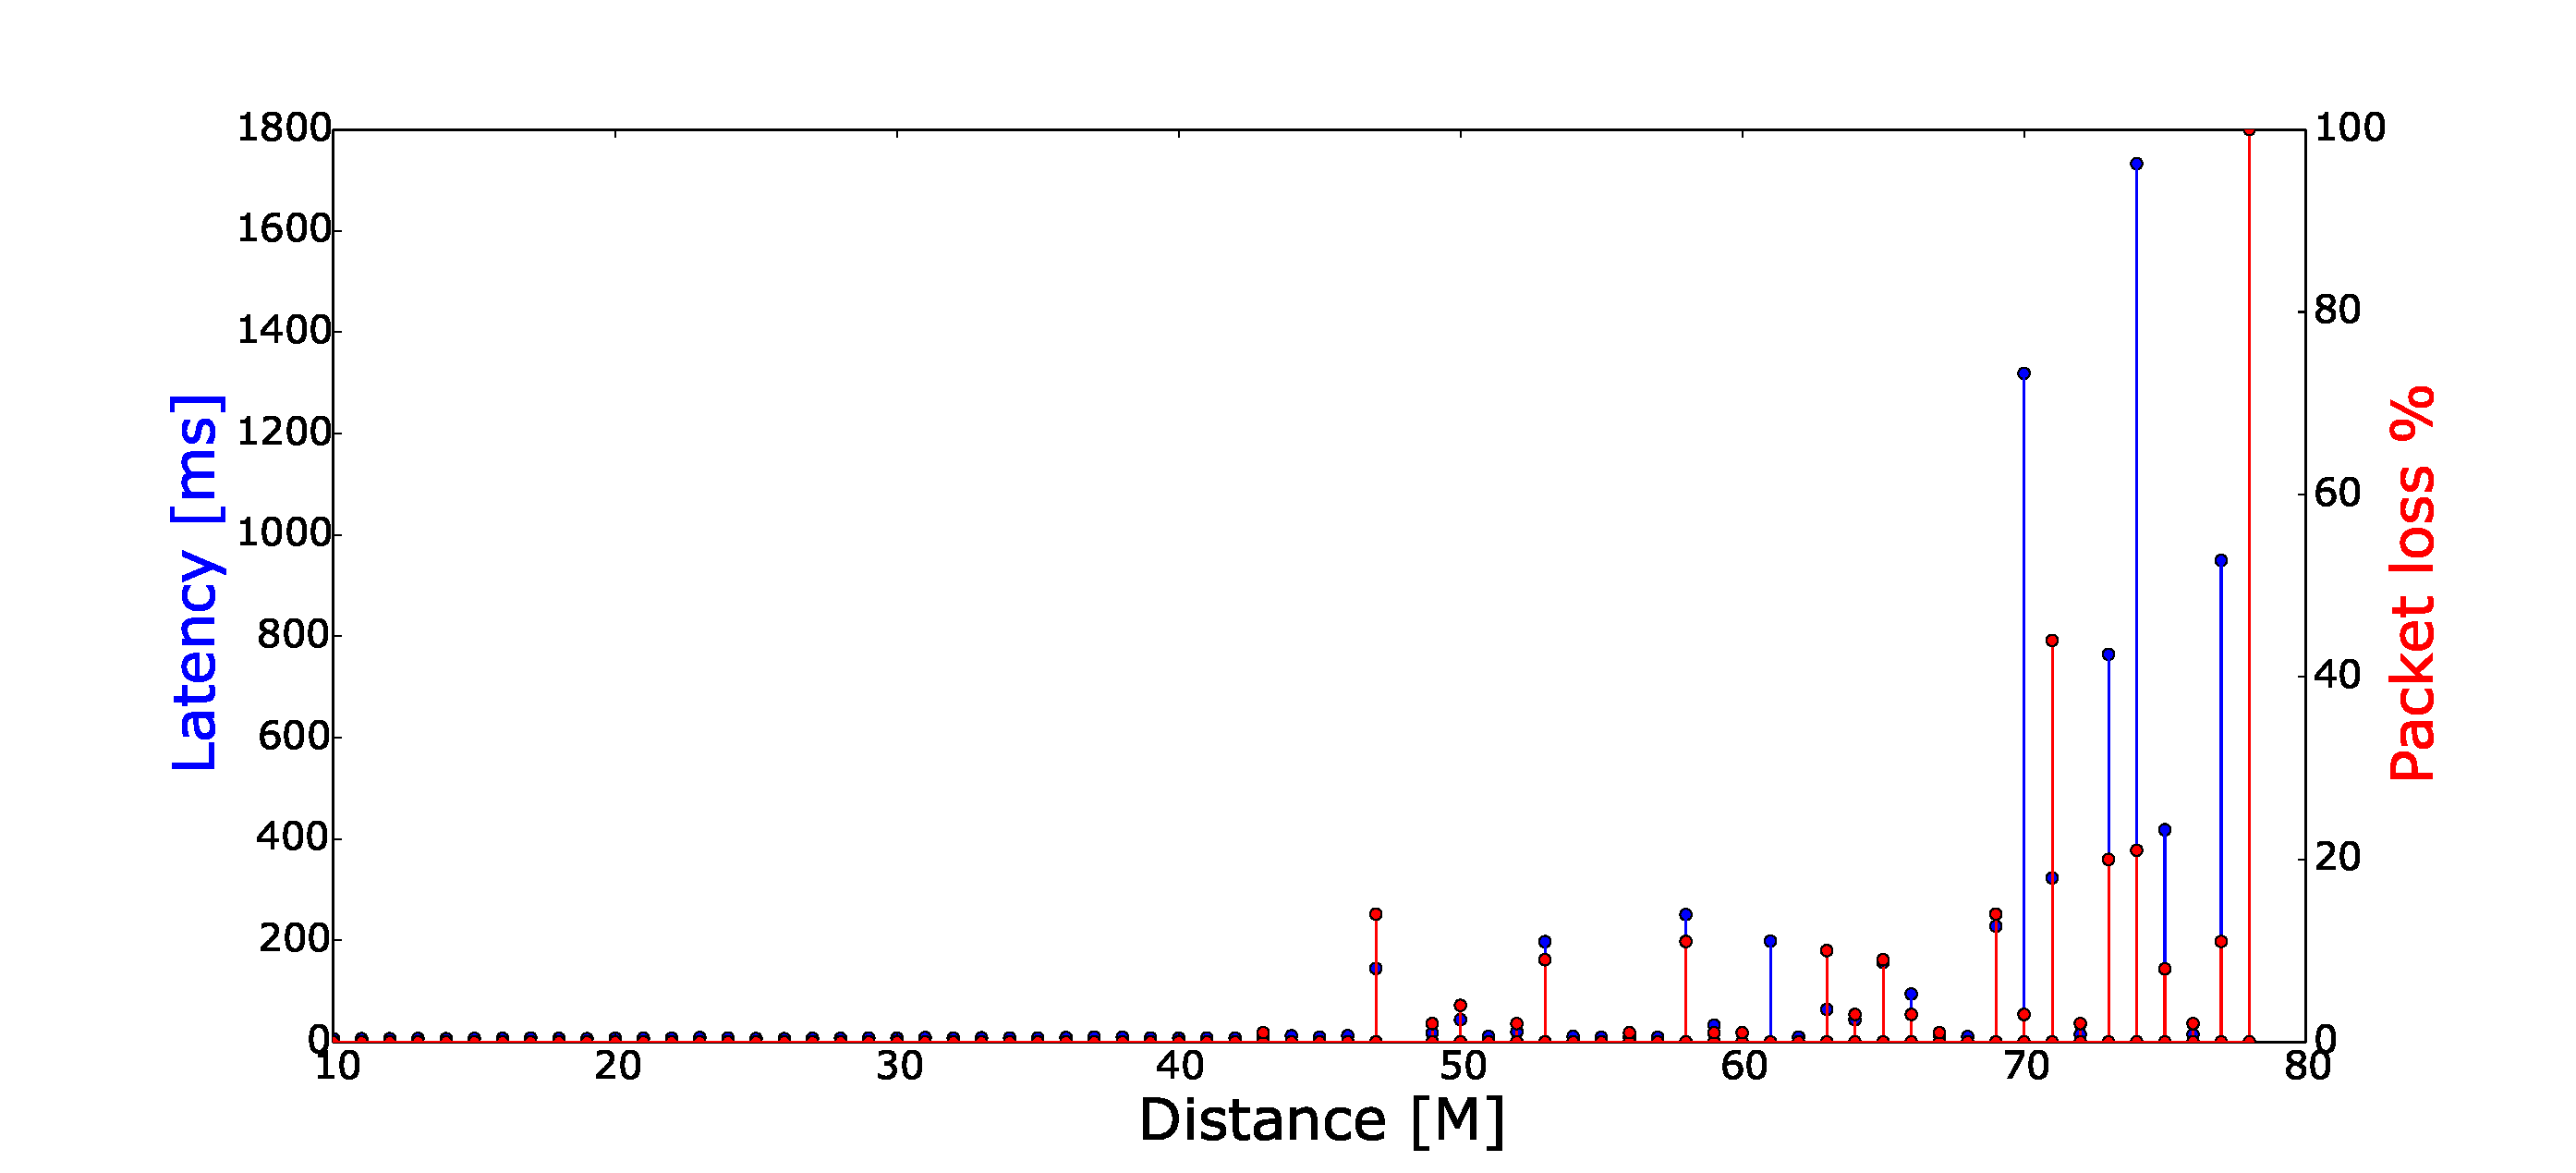
\includegraphics[width=1\textwidth]{graphics/wifi_test_latency_1.eps}
  \caption{Plot shows the latency, packet loss vs. distance. Up until 46 meters no packets are dropped and the latency is quite low.}
    \label{fig:wifi_pingtest}
\end{figure}


\section{WIFI range with CRC} \label{sec:result_wifi_range_crc}
\begin{figure}[H]
    \center
    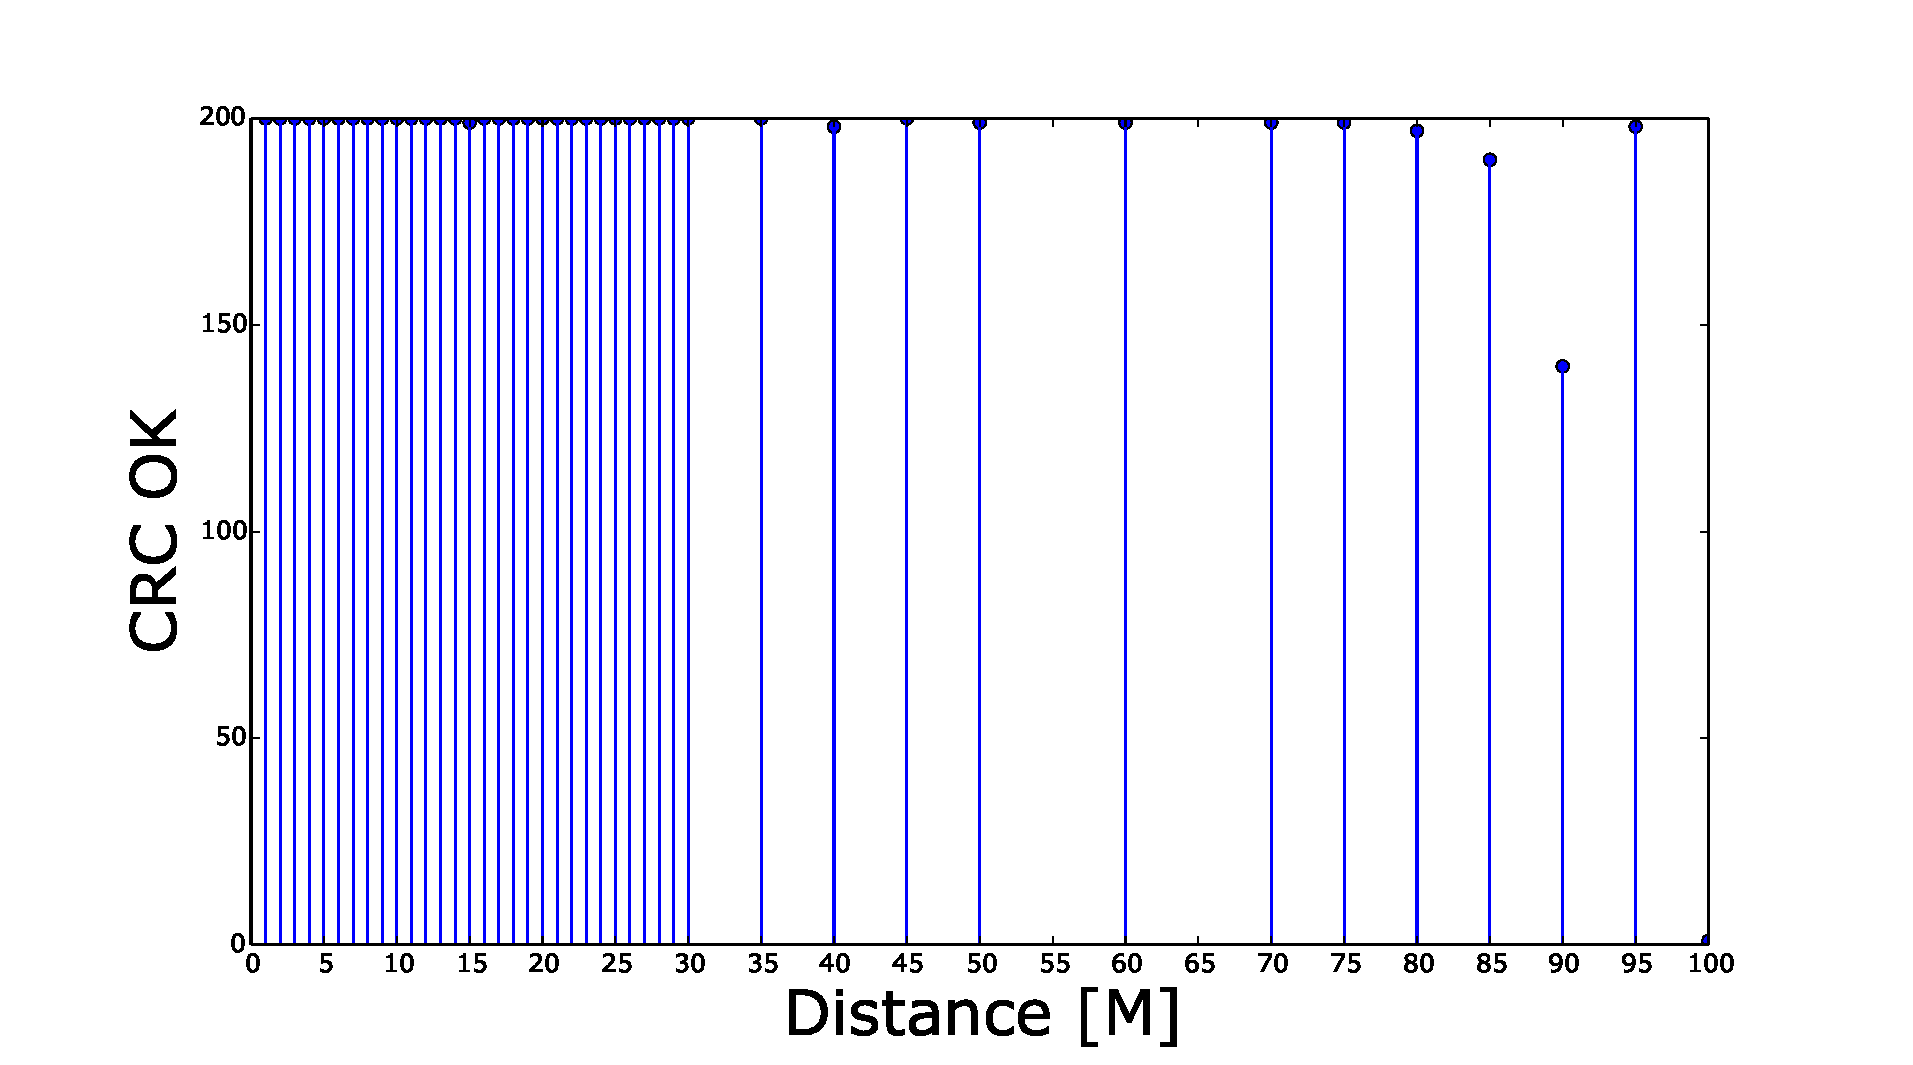
\includegraphics[width=0.85\textwidth]{graphics/crc_distance_check.eps}
	\caption{Measurements was initially done at every meter, however to save time the distance was increase to 5 meter and later to 10. When packets began to drop, measurements was done at 5 meter interval again. At 100 meters the WIFI connection was dropped.}
    \label{fig:wifi_crc_check}
\end{figure}




\section{WIFI with two extension-boards} \label{sec:result_two_wifi_modules}
\begin{table}[]
\centering
\caption{My caption}
\label{my-label}
\begin{tabular}{@{}|l|l|l|l|l|@{}}
\toprule
         & Test 1 & Test 2 & Test 3 & Test 4 \\ \midrule
Module 1 & 200    &        & 200    &        \\ \midrule
Module 2 &        & 200    &        & 200    \\ \bottomrule
\end{tabular}
\end{table}
 

\chapter{Discussion}\label{chp:discussion}
It is possible to design a indoor and outdoor positioning system using the same \ac{AQ} firmware.
The system was designed to be scalable so that more drones can be controlled by the system.
By using ROS on the PC the system is modular designed so that the behavior of the drones can be changed without the need of replacing or editing other working components of the system. A \textit{Decision\_Maker} nodes was made to handle coordinate conversion and control the drones. By moving a 4 order marker along a rectangle in the flight-plane the size of the rectangle can be estimated with an error of 1.2 and 0.9 in with and height respectively. 
The ESP8266 wireless module was chosen based on requirements such as weight, size, documentation available and price. The ESP8266 got the highest score and was mainly chosen since it is a widely used module on the internet. An extension-board was created to act as a bridge between the PC and the drone with an At90CAN128 microcontroller. The At90CAN128 was chosen based on its build-in CAN-controller, its availability, and because of previous experience. Three tests was conducted to test the performance of the ESP8266 wireless module. If the distance is larger than 46 meters the tests shows the latency begins to increase and the CRC packets will arrive without error but will be delayed. If the distance is larger than 85 meters the packets suffers from high latency and errors starts to occur.
By selecting a \ac{RTCS} scheduler for the At90CAN128 it was possible to run a task every second with a mean and standard deviation of 1.0089 and 0.0042 sec. respectively. By creating a task-diagram it was possible to design a modular firmware for the At90CAN128 and to use queues as communication between the tasks. Furthermore a small firmware without a scheduler for the EPS8266 module were written.
Several tests were made in order to verify the CAN-GNSS injection worked. First by doing tests indoor and then moving the testing outside.
The outdoor tests shows it is possible to inject CAN-GNSS positions into \ac{AQ} and that \ac{AQ} can be told how much its UKF should trust the GNSS positions based on the DOP values.
When using the MarkerLocator with the improved order detection it is possible to detect two drones without having false positive/negative. By making a test of the distance between two markers there was an error of 0.81 cm.





\chapter{Conclusion}\label{chp:conclusion}
It can be concluded that it was possible to design a generic system architecture where locations can be injected over CAN into the AQ M4-board using different sources of localization. Tests were conducted in order to verify it was possible to inject absolute positions into AQ. An outdoor test with an RTK-GNSS used in the scientific paper reveals that it works and there by indicates that it also works with a indoor localization system.
An extension-board was created capable of acting as a bridge between a PC and a drone in order to send absolute positions to the AQ-firmware. The extension-board was able to receive 200 packets without CRC error at 10 hz at a distance of 46 meters without loosing any packets or experiencing any noticeable latency. By using the extension-board the 4 drones should be able to fly at a distance between each other of $\pm$ 10 cm without loosing any positions. The communication was also tested with two extension-boards which indirectly verifies the scalability in ROS and the design of the indoor system architecture. This suggests that it also works with 4 drones.
 The MarkerLocator was used as indoor localization and was modified in order to be able to verify the right order was detected. The MarkerLocator showed an accuracy of 0.81 cm which suggests that keeping a distance between 4 drones of $\pm$ 10 cm is possible using the MarkerLocator.\\

Due to lack of time and because of the time spend on the outdoor RTK-GNSS it was not possible make 3 drones follow a leader. Therefor the hypothesis can not be accepted nor rejected since the subparts made fulfills the requirements and suggests it works with the 4 drones.\\

To make it work the system needs to be put together and verify one drone can be controlled. If so, test with more drones and at least replace the current \textit{Decision\_Maker} with a leader-follower algorithm. In case the drone is not capable of holding its height very accurately a distance sensor should be connected on the extension-board. If more advanced control algorithms should be implemented, it might be less resource demanding if the coordinate conversion is moved into two other node, before and after the \textit{Decision\_Maker}-node.
If controlling multiple drones it will fast be an issue concerning the MarkerLocator. An efficient way to lover the amount of resources required would be to port the MarkerLocator into C++.


% --------- End Matter --------- %

\newpage
\listoffigures
%\begingroup
%\let\clearpage\relax
\newpage
\listoftables
%\endgroup
%\printbibliography
\bibliography{bibliography}
\begin{appendices}
\makeatletter
\addtocontents{toc}{\let\protect\l@chapter\protect\l@section}
\makeatother
\makeatletter
\addtocontents{toc}{\let\protect\l@section\protect\l@subsection}
\makeatother
\addtocontents{toc}{\protect\setcounter{tocdepth}{1}} % Exclude everthing from \section and downwards from ToC
\captionsetup{list=no} % Exclude all figures and tables from LoF and LoT


%\bibliographystyle{ieeetr}
\bibliographystyle{IEEEbib}
%\bibliography{bibliography}


% Chapter 2 Hardware:
% Chapter 3 Vision:
%\input{app_camera_calibration}
%\input{app_evs_object_detection}
%\input{app_distance_calculation}
%\input{app_opencv_functions}
%\input{app_canny_edge}

% Chapter 4 Communication:
%\input{app_dual_rpi_speed}
%\input{app_K827P_speed}

% Chapter 5 UR5 Controller System:
%\input{app_final_implementation_benchmark}


\end{appendices}
\section{AutoQuad CAN protocol}
In order to spoof the onboard GPS, the CAN-bus was chosen as input to AQ. 
The CAN-bus is already implemented and widely used on a ViaCopter drone to communicate between AQ and hardware like ESCs, PDB etc. Much time was spend reading through the source code and trying to figure out how the protocol works.
The developers behind AQ says, that the code is the documentation and thereby have not written any real documentation. \\
Figuring out how it works was done using debugging utilities such as breakpoints and looking at the content of the different memory locations in CrossWorks.\\
More debugging tricks can be seen in appendix \ref{app:debugging}. 
To further investigate the protocol a PEAK-CAN adapter were connected to a Ladybird drone and several python scripts were developed to send and receive messages from AQ. \\
The author did not go into details about messages used between AQ $\leftrightarrow$ ESC's and AQ $\leftrightarrow$ OSD.\\

\subsection{CAN Protocol description}
A Peak-CAN adapter were used throughout the project. It supports High-speed ISO 11898-2\footnote{\url{http://www.peak-system.com/PCAN-USB.199.0.html?&L=1}} which is a standard that states the properties of physical layer. 
Its max speed is 1 mbit which is the speed AQ uses to communicate on the CAN-bus. 
AQ uses CAN 2.0B which has 29 identifier bits.
AQ is not using an existing protocol on top of ISO 11898-2. The developers created their own to suit their needs.\\

\subsubsection{Identifier bits}
A Generic look at a AQ CAN messages can be seen in table \ref{tab:can_identifier_bits}.
The normal function of the identifier bits is the priority of the messages.
A CAN controller can then be setup to only allow certain messages to be processed depending on their identifier bits.
The identification bits has been split up in AQ to contain information about the sender, receiver etc. Which is not normally saved information in a CAN message.
\begin{table}[H]
\resizebox{\textwidth}{!}{%
	\begin{tabular}{|c|c|c|c|c|c|c|c|}
	\hline
	\multicolumn{8}{|c|}{CAN Message} \\ 
	\hline
	 \multicolumn{7}{|c|}{Identfier bits [29 bits]} &  		\multicolumn{1}{c|}{Data bits [max 64 bits]} \\
	 \hline
	 LCC [28:27] & TT [26] & FID [25:22] & DOC [21:16] & SOID 	[15:11] & TID [10:16] & SEID [5:0] & \\
	\hline
\end{tabular}}
	\caption{Table shows the identifier bits used in AutoQuad CAN messages}
	\label{tab:can_identifier_bits}
\end{table}

In figure \ref{tab:abbri_can_msg} the abbreviations can be seen.
\begin{table}[H]
		\begin{tabular}{|l|l|}
		\hline
		LCC & Logical Communications Channe \\
\hline
		TT & Target Type \\
\hline
		FID & Function ID \\
\hline
		DOC & Data Object Code \\
\hline
		SOID & Source ID \\
\hline
		TID & Target ID \\
\hline
		SEID & Sequence ID \\
\hline
		\end{tabular}
		\caption{Table shows 
abbreviations used in table \ref{tab:can_identifier_bits}}
		\label{tab:abbri_can_msg}
\end{table}

Each of the elements in an AQ messages will be explained how they are used in AQ. \\

\subsubsection{Logic Communication Channel}
LCC is the priority of the message. 
To understand how LCC works, one needs to look into CAN arbitration.
As stated in ISO-11898-2, a 0 is the dominant bit and a 1 is the recessive bit.
The example in figure \ref{tab:can_arbitration} shows two nodes each transmitting a packet.
The arbitration only happens during the transmission of the identifier bits.
In the example on bit 8, Node 16 losses the arbitration and stops transmitting.
Node 15 keeps transmitting its packet because it has lower identifier bits and thereby higher priority.
\begin{figure}[H]
    \center
    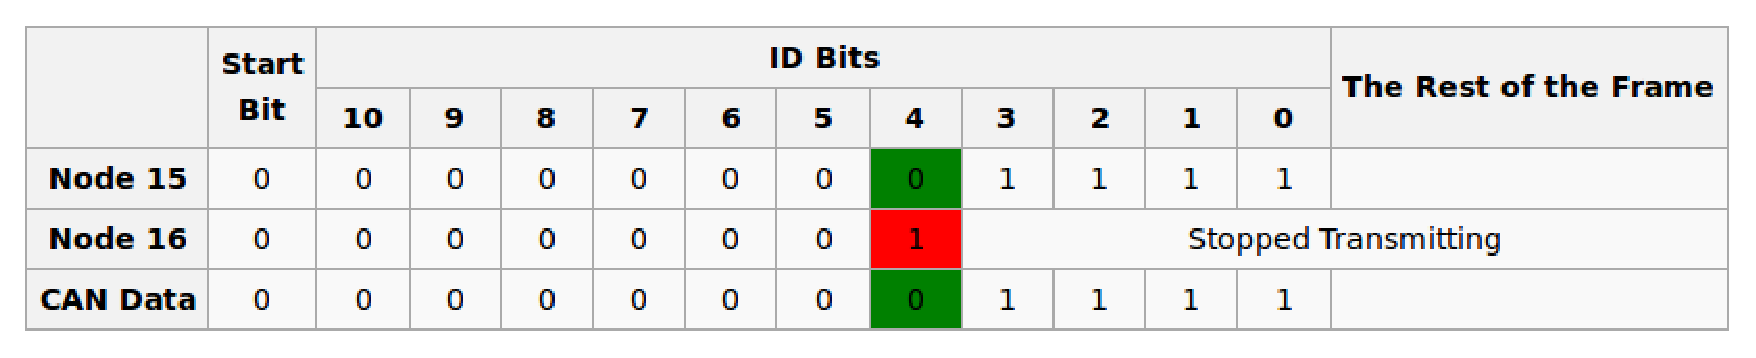
\includegraphics[width=1\textwidth]{graphics/can_arbitration.eps}
    \caption{Example of CAN arbitration where node 15 has the lowest ID and thereby highest priority}
    \label{tab:can_arbitration}
\end{figure}
\newpage
LLC in a message can take one of the defines in code \ref{code:llc_defines}
\begin{lstlisting}[language = c, caption = LLC defines, label=code:llc_defines]
#define CAN_LCC_EXCEPTION   ((uint32_t)0x0<<30)
#define CAN_LCC_HIGH        ((uint32_t)0x1<<30)
#define CAN_LCC_NORMAL      ((uint32_t)0x2<<30)
#define CAN_LCC_INFO        ((uint32_t)0x3<<30)
\end{lstlisting}

\begin{table}[H]
\centering
\caption{Table showing the 4 types of priority in AQ}
\label{my-label}
\begin{tabular}{|l|l|l|}
\hline
\textbf{Name} & \textbf{Value} & \textbf{Priority (lowest first)} \\ \hline
EXCEPTION     & 0000           & 0                 \\ \hline
HIGH          & 0001           & 1                 \\ \hline
NORMAL        & 0010           & 2                 \\ \hline
INFO          & 0011           & 3                 \\ \hline
\end{tabular}
\end{table}

\subsubsection{Target Type}
Target type can either be “node” or “group” depending on if the receiver(s) is one or more nodes. 
\begin{lstlisting}[language = c, caption = Target type defined in AQ, label=code:target_types]
#define CAN_TT_GROUP        ((uint32_t)0x0<<29)
#define CAN_TT_NODE         ((uint32_t)0x1<<29)
\end{lstlisting}
The GROUP is used when AQ sends its reset-msg upon startup.\\
When the authors node sends a sensor-measure to AQ it will be of type CAN\_TT\_NODE.
\subsubsection{Function ID}

Function ID describes the function of the CAN message. If it is a PING, ACK, NACK, etc.
It simply states the function of packet so the receiver node knows what to do with the message.
Different types of functions can be seen in code \ref{code:function_defines}
\begin{lstlisting}[language = c, caption = Excerpts from AQ's list of function defines, label=code:function_defines]
#define CAN_FID_RESET_BUS		((uint32_t)0x0<<25)
#define CAN_FID_ACK				((uint32_t)0x1<<25)
#define CAN_FID_REQ_ADDR		((uint32_t)0x7<<25)
#define CAN_FID_GRANT_ADDR	((uint32_t)0x8<<25)
#define CAN_FID_CMD           ((uint32_t)0x3<<25)
\end{lstlisting}

Table \ref{tab:fid_descriptions} describes the FIDs shown in listing \ref{code:function_defines}. \\

\Mathias{Dette er forkert, eftersom alle defines er taget fra AQ's can.h så der passer det..}
If a message is if FID CAN\_FID\_CMD, the Data Object code will be used as the command.\\
It should be noted from code \ref{code:function_defines} that the FID's is moved 25 positions to the left but FID is shown in table \ref{tab:can_identifier_bits} is at bits 22:25. 
The offset of three bits is due to the way ARM's CAN registers is implemented. The three initial bits in CAN\_TIxR and CAN\_RIxR (registers used to transmit and receive respectively) \footnote{\url{http://www2.st.com/content/ccc/resource/technical/document/reference_manual/59/b9/ba/7f/11/af/43/d5/CD00171190.pdf/files/CD00171190.pdf/jcr:content/translations/en.CD00171190.pdf:688}} registers are general information about the CAN messages like whether it is extended (Part B.0) or not.
\begin{table}[H]
\centering
\caption{Descriptions of the FIDs mentioned in code \ref{code:function_defines}}
\label{tab:fid_descriptions}
\resizebox{\textwidth}{!}{%
\begin{tabular}{@{}|l|l|@{}}
\toprule
\textbf{FID}          & \textbf{Description}                                                               \\ \midrule
CAN\_FID\_RESET\_BUS  & Message sent by AQ when powered up                                                 \\ \midrule
CAN\_FID\_ACK         & Message sent to AQ when acknowledging a received message                           \\ \midrule
CAN\_FID\_REQ\_ADDR   & Messaged used when a node on the bus tries to register itself as a node on the bus \\ \midrule
CAN\_FID\_GRANT\_ADDR & Messaged sent by AQ when it registers a node as a node on the bus.                 \\ \bottomrule
\end{tabular}
}
\end{table}

Table \ref{tab:fid_descriptions} shows a description of the 4 FIDs used when a node is registered. 

\subsubsection{Data Object Code}
Data Object code is used as a parameter to the FID. Data Object Code can have different values depending on the fid. Code \ref{code:doc_useage} shows a function using DOC when message FID is CAN\_FID\_CMD.

\begin{lstlisting}[language = c, caption = Snippet of AQ's can.c:365, label=code:doc_useage]
void canProcessCmd(... ,uint8_t doc, ...) {
    switch (doc) {
        case CAN_CMD_STREAM:
        	...
            break;
        case CAN_CMD_TELEM_VALUE:
        	...
            break;
        case CAN_CMD_TELEM_RATE:
        	...
            break;
    }
}
\end{lstlisting}

In section \ref{sec:reg_aq_node} DOC is used by the author to tell which part of the GPS data is getting sent but where FID is CAN\_FID\_TELEM.
\Mathias{Fixe ref til section om GPS spoof}

\subsubsection{Source/Target/Network ID}
When referred to source/target ID but without respect to either sender or receiver but just a CAN-node, then it is referred to as NetworkId. When a node registers itself in AQ, it gets assigned a NetworkId.

\subsubsection{Sequence ID}
The sequence id is incremented on transmission of each message. It is used when eg. 
A CAN-node sends a reply to a get-message, it is then including the sequence id of the get-message so AQ knows what it receives a reply for.

\subsubsection{Data bits}
The data bytes does not have a general definition, it depends on the function id. With some FIDs the data field may contain additional parameters.\\ \\
Eg. When FID is CAN\_FID\_REQ\_ADDR, data has the fields shown in table \ref{tab:packet_from_node}
\begin{table}[H]
\centering
\caption{Packet sent from node when registering in AQ}
\label{tab:packet_from_node}
\begin{tabularx}{0.92\textwidth}{@{}|X|X|X|X|X|X|X|X|@{}}
\toprule
\multicolumn{8}{|c|}{64 bits}                           \\ \midrule
0 & 0 & CanId & CanType & UUID3 & UUID2 & UUID1 & UUID0 \\
\midrule
7 & 6 & 5 & 4 & 3 & 2 & 1 & 0 \\ \bottomrule
\end{tabularx}
\end{table}

\textbf{UUID} is a unique address generated by each node on the bus. In ESC32v2\footnote{\url{https://github.com/bn999/esc32/blob/master/onboard/can.c}} the address is calculated using XXH-hashing algorithm. The algorithm generates a 32 bit hash from a given input value and a salt.
The input to XXH in ESC32v2 is the unique ID that every ARM in the STMF32\footnote{\url{http://www2.st.com/content/ccc/resource/technical/document/reference_manual/59/b9/ba/7f/11/af/43/d5/CD00171190.pdf/files/CD00171190.pdf/jcr:content/translations/en.CD00171190.pdf}}
 family has. Code \ref{code:xxh_canesc32v2} shows how it is implemented in AQ.

\begin{lstlisting}[language = c, caption = Snippet showing UUID generated in ESC32v2, label=code:xxh_canesc32v2]
can.h:20
#define CAN_UUID	0x1FFFF7E8

can.c:753
canData.uuid = XXH32((void *)CAN_UUID, 3*4, 0);
\end{lstlisting}

\textbf{CanType} is the type of the node trying to register. Eq. SENSOR, ESC and SERVO.  \\

\textbf{CanID} is the number of the CanType node trying to register. When an ESC32v2 is trying to register it sends CanId as the ESC number ranging from 1 to the number of ESC's mounted on the drone. The CanID is assign to each ESC manually as part of the configuring.

% redefine the \mess so that \_ works...
\renewcommand{\mess}[4][0]{
  \stepcounter{seqlevel}
  \path
  (#2)+(0,-\theseqlevel*\unitfactor-0.7*\unitfactor) node (mess from) {};
  \addtocounter{seqlevel}{#1}
  \path
  (#4)+(0,-\theseqlevel*\unitfactor-0.7*\unitfactor) node (mess to) {};
  \draw[->,>=angle 60] (mess from) -- (mess to) node[midway, above]
  {#3};
}

\subsection{Registering a node in AQ}\label{sec:reg_aq_node}

When the AQ is starting up, it is transmitting a CAN\_FID\_RESET\_BUS to the bus.
When each CAN-node receives the messages, they send out a CAN\_FID\_REQ\_ADDR message in order to get registered as a node in AQ.
If a node on the bus does not get registered it will not be able to communicate with AQ. \\
When AQ receives an CAN\_FID\_REQ\_ADDR, it sends back a CAN\_FID\_GRANT\_ADDR to tell the node that the registration is successful and to assign the node its networkID.
This id is used later to identify the node when it is transmitting a message or when AQ wants to send out a message to that specific node.
The sequence diagram in figure \ref{fig:protocol_req_node} shows the described sequence.

\begin{figure}[H]
    \center
      \begin{adjustbox}{max width=0.5\textwidth}
	\begin{sequencediagram}
	  \newthread{0.4}{pynode}{ROS-node}
	  \newthread{7}{autoquad}{AutoQuad}

	  \mess[1]{autoquad}{CAN\_FID\_RESET\_BUS}{pynode}

	  \begin{call}[3]{autoquad}{Wait(100ms)}{autoquad}
			\postlevel
			\postlevel
			\mess{pynode}{CAN\_FID\_REQ\_ADDR}{autoquad}
			\postlevel
			\mess{autoquad}{CAN\_FID\_GRANT\_ADDR}{pynode}
	  \end{call}
	  \mess{autoquad}{CAN\_CMD\_TELEM\_VALUE}{pynode}
	  \mess{pynode}{ACKValue*}{autoquad}
	  \postlevel

  	  \mess{autoquad}{CAN\_CMD\_TELEM\_RATE}{pynode}
  	  \mess{pynode}{ACKRate}{autoquad}
	\end{sequencediagram}
	\end{adjustbox}
	\caption{Registering a new node in AQ}
	\label{fig:protocol_req_node}
\end{figure}

Depending on the canType set in the data-field when a node is transmitting a CAN\_FID\_REQ\_ADDR, AQ might send zero or more messages back to the node.\\
In figure \ref{fig:protocol_req_node} it can be seen that AQ sends back CAN\_CMD\_TELEM\_VALUE and CAN\_CMD\_TELEM\_RATE because the CanType is set to SENSOR.
Each of the two messages has two fields in the data field, that contains information about the stream.
CAN\_CMD\_TELEM\_VALUE is used to request telemetry from a node that registered itself as a SENSOR. 
CAN\_CMD\_TELEM\_RATE is the requested telemtry rate from AQ. Default is 10 hz \footnote{https://github.com/bn999/autoquad/blob/master/onboard/canSensors.h:24}. \\
A timeout timer is started when each message has been sent. 
If an ACK is not received after each message within 250 ms \footnote{https://github.com/bn999/autoquad/blob/master/onboard/can.h:71} a timeout counter is incremented. At the time of writing this information is not used but might be later on.\\

Code in \ref{code:aq_req_extend_time} shows a snippet\footnote{\url{https://github.com/bn999/autoquad/blob/master/onboard/can.c:547}} from AQ where AQ waits for nodes to request an address.

\begin{lstlisting}[language = c, caption = Snippet showing AQ waits for devices, label=code:aq_req_extend_time]
canResetBus();

// wait 100ms for nodes to report in
micros = timerMicros() + 100000;
while (timerMicros() < micros)
    // extend wait period if more nodes found
    if (canCheckMessage(0))
        micros = timerMicros() + 100000;
\end{lstlisting}

AQ waits default 100 ms for nodes to request an address. If canProcessMessage() returns true a node tried to register and the registration period is extended 100 ms.
 
\subsection{Registering node test} \label{sec:reg_node_test}
Implementation of a CAN-node running on a PC was initially done in python. The python module \textit{SocketCan} \footnote{\url{http://python-can.readthedocs.io/en/latest/socketcan_native.html}} supports PeakCAN adapter out of the box.\\

Code \ref{code:python_reg_node} shows a snippet of main.py.

\begin{lstlisting}[language = python, caption = Snippet showing AQ registration from python, label=code:python_reg_node]
# Create autoquad handle
autoquadNode = AutoQuadNode('can1', 'socketcan')

# Wait for reset msg transmitted by AQ.
autoquadNode.WaitForReset(timeout=1000);
print "Recevied readymsg"

# Register node, CanType as sensor and CanID as PDB ampere
msg = autoquadNode.RegisterNode(CAN_TYPE_SENSOR, CAN_SENSORS_PDB_BATA)

# Wait for telemetryTryValue
msg = autoquadNode.recv()
# Parse message
msg = CanMessage(msg)

# Print all values received, _str__(self) overwrited
print msg

# ACK TelemValue
autoquadNode.AnswerRequestTelemValue(msg)

# Wait for telemetryRate
msg = autoquadNode.recv()

# Parse message
msg = CanMessage(msg)

# ACK TelemRate
autoquadNode.AnswerRequestTelemRate(msg)
\end{lstlisting}

When a node has successfully registered, it is shown in QgroundStation as shown in figure \ref{fig:successful_register}.
It can be seen 4 motors were connected to the CAN bus, but also that the spoofed sensor was registered.

\begin{figure}[H]
    \center
    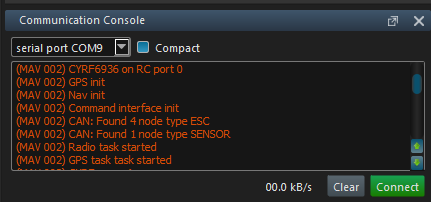
\includegraphics[width=0.5\textwidth]{graphics/test_register_node.png}
    \caption{Successful SENSOR registration}
    \label{fig:successful_register}
\end{figure}

\subsection{Spoofed current test}
When an AQ PDB is mounted on a drone, the PDB measures voltage, current and temperature and sends the measurements to AQ where they get logged.\\
The code in section \ref{sec:reg_node_test} was further developed into a sensor simulator that spoofs current measurements into AQ to test the registering works probably. \\
A logger extension-board was mounted on the M4-board in order to save the measurements to a MicroSD-card.

Code \ref{code:spoof_current} shows the implementation where a sinus is generated to simulate a current and how it is transmitted to AQ.

\begin{lstlisting}[language = python, caption = Snippet spoofing current measurements into AQ, label=code:spoof_current]
def ReqistrerTelem(self):
	# self.sinus is a list of sinus values
	sensor_value = self.sinus[self.phase]

	# Get next value next time and do overrun
	self.phase+=1
	self.phase = self.phase % 20

	# Pack as IEEE754 float
	sensor_value_float = pack('>f', sensor_value)

	# Create list of float-bytes as integers
	data_float = [int(ord(elm)) for elm in sensor_value_float]

	# Reverse list and append empty data
	data_float.reverse()
	
	# Send to AQ. id =  CAN_FID_TELEM (02c00000) | Sourceid 1 (00000800) | CAN_SENSORS_PDB_BATA (00004000)
	self.send(0x02c04800, data_float)
\end{lstlisting}

The method defined in code \ref{code:spoof_current} was run every 100ms.\\
After the code ran for a few seconds the SD card was plugged into a PC and QgroundStation configured to make a plot of the PDB\_CURRENT-field. The plot can be seen in figure \ref{fig:pdb_current_log} 


\begin{figure}[H]
    \center
    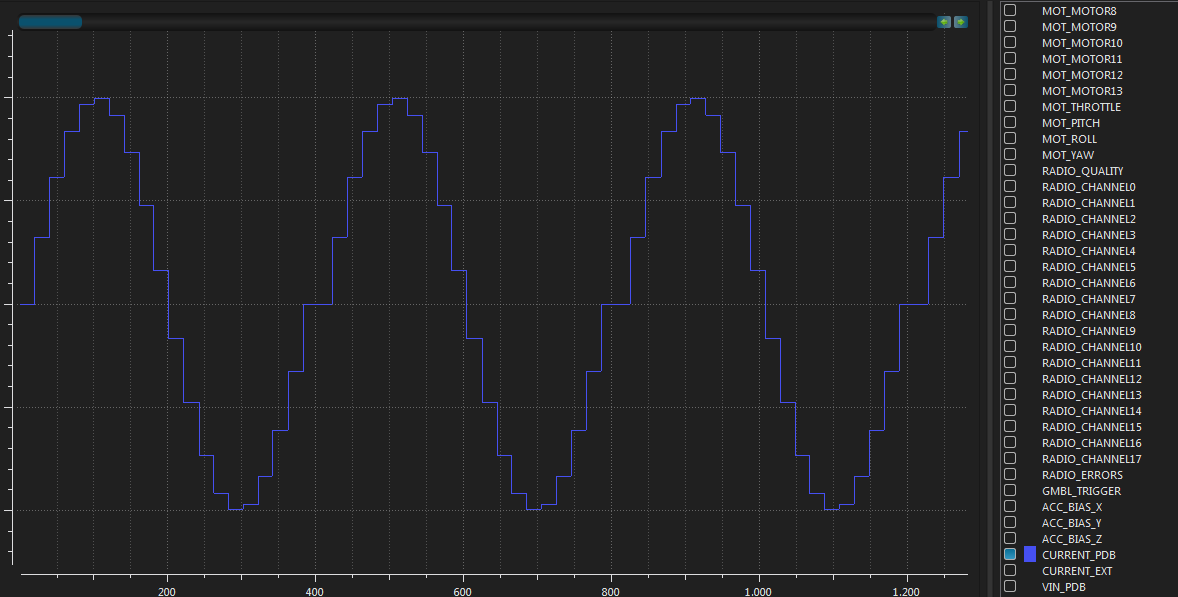
\includegraphics[width=0.8\textwidth]{graphics/test_can_spoof_current.png}
    \caption{Test of python CAN test}
    \label{fig:pdb_current_log}
\end{figure}

Figure \ref{fig:pdb_current_log} shows the sinus generated from the node as expected.


\newpage


\section{Test of spoofed GNSS}
Testing of the spoofed GNS was split intro two subtests. \\
The first test was conducted in order to validate the GPS spoofing using the CAN-bus works when the drone is laying on a table. \\
Test 1 can be seen in \ref{sec:test_of_spoofed_positions_indoore}.\\
The second test was conducted as the first test, but when the drone is airborn.\\
Test 2 can be seen in \ref{sec:test_of_spoofed_positions_outdoore}



----------------------------------\\
Figure Y shows the waypoint list uploaded to the drone. It is expected that the drone will behave as if it was using its onboard GPS.
The GPS positions will be gathered in a rosbag to be used later on in test2.
A flight with the onboard GPS will be done in order to have a reference flight.\\
\textbf{Testx}
Test two will be conducted much the same way as test1. However the GPS will be replaced with a lightweight RTK GPS. The RTK GPS positions will also be saved in a rosbag for later analyse. Is is expected that when using the RTK GPS the drone is closer to its waypoints  shown in figure Y, than when using a normal GPS.

----------------------------------\\




bstract.tex


\subsection{Test of spoofed positions indoore}
\label{sec:test_of_spoofed_positions_indoore}
\textbf{Introduction}
The purpose of this test was to see if the GPS coordinates was spoofed correctly and read probably by AQ and to validate the ROS node responsible for creating CAN messages was working as long as the drone is laying on a table. If this works, it shows that the UKF works with the spoofed coordinates as expected, and that the author of the report can spoof the GPS position from a vision based localization system. \\

A rosbag was used to collect data from the GPS since it publishes data to a topic when played as a node did when the recording took place. This results in no code has to be written and when the code works with a rosbag it also works when it is replaced with a node providing real-world data. \\

\textbf{Test}
\begin{figure}[H]
    \center
    \includegraphics[width=0.8\textwidth]{graphics/Indoore_test_spoofed_can.png}
    \caption{Block schematic of the connected components}
    \label{fig:test_block}
\end{figure}


Figure\ref{fig:test_block} shows the connected componenets. 


To get the NMEA strings from the GPS, an already existing Frobomind component will be used. It reads from a serial port, and publishes the parsed NMEA string to \textit{/fmData/nmea\_from\_gps}. Rosbag was then used to save the messages.
The code written by the author will then subscribe to \textit{/fmData/nmea\_from\_gps} and publish the CAN-messages to another topic. A third node which is also a part of Frobomind will then subscribe and send the CAN-messages.

\begin{figure}[H]
    \center
    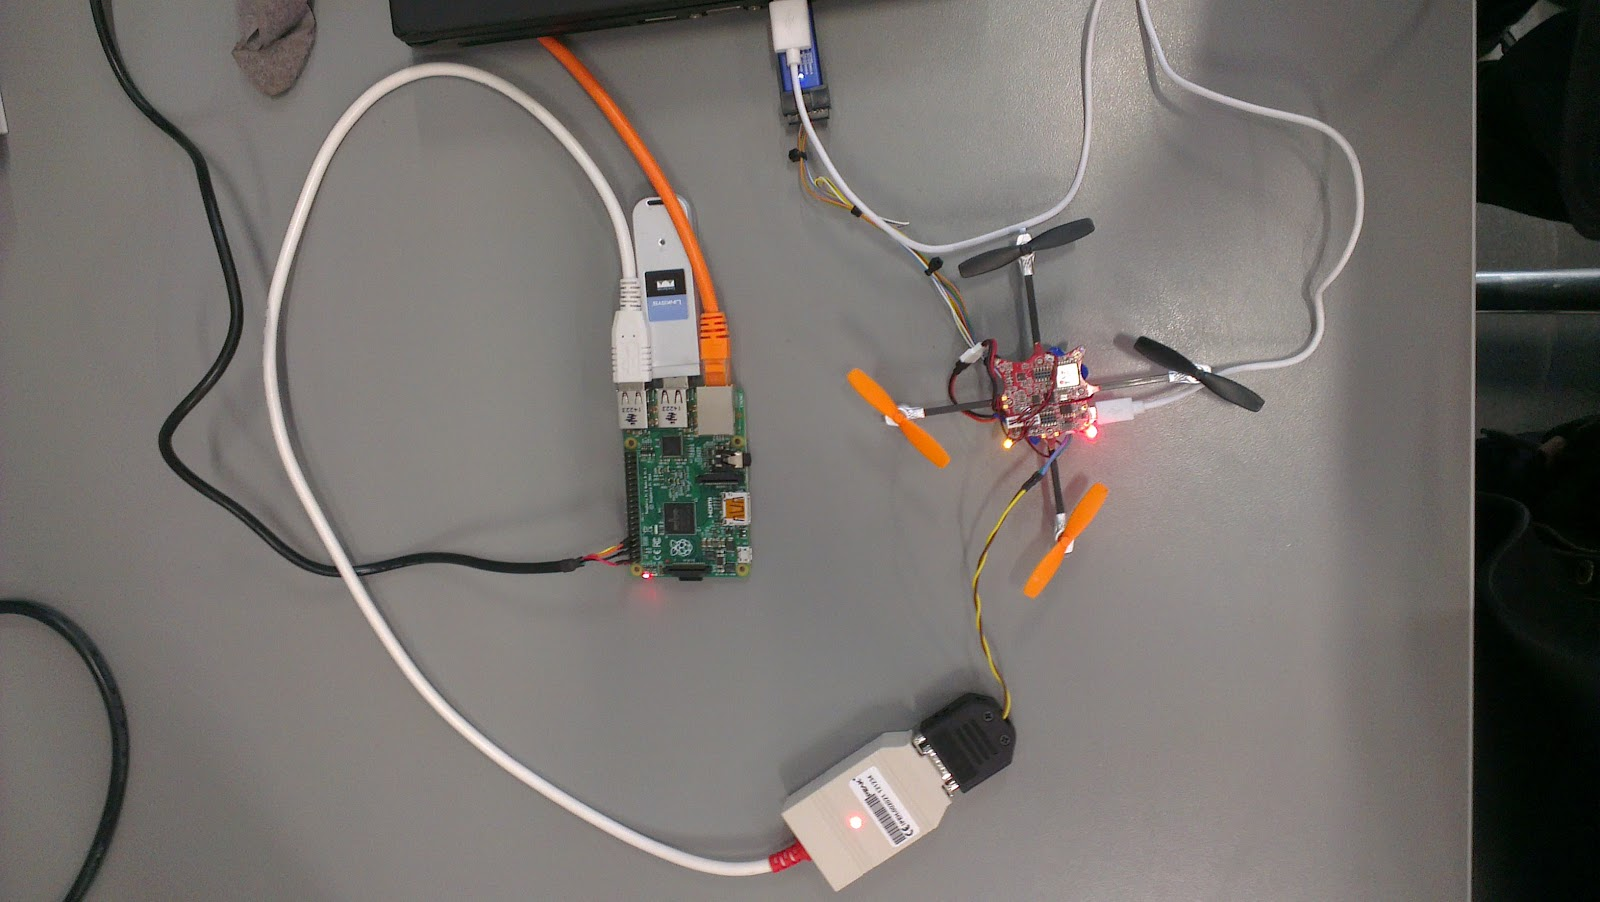
\includegraphics[width=0.6\textwidth]{graphics/test_test_setup_hw.jpg}
  \label{fig:boat1}
  \caption{Test-setup shown}
\end{figure}


The Rpi is connected directly to the PC using the orange ethernet cable.
The rosbag was stored and played on the PC, so the ethernet cable were used to share rostopics between the PI and the PC. The roscore where running on the PC.\\
The Ladybird drone is connected to the RPI using a PEAK CAN-adapter to transfer CAN messages. The Ladybird is powered by the white USB-cable and to show the position of the drone in QgroundStation. The PC is connected to the drone using ST-Link SWD to easier start, stop and restart the drones firmware during the test. To access a TTY on the PI, an FTDI cable has been connected to the PC.


In order to obtain GPS-testdata to spoof into AQ, a rosbag was used to record data collected by the GPS mounted on the authors laptop. The setup can be seen in figure \ref{fig:test_laptop_and_gps} 
\begin{figure}[H]
    \center
    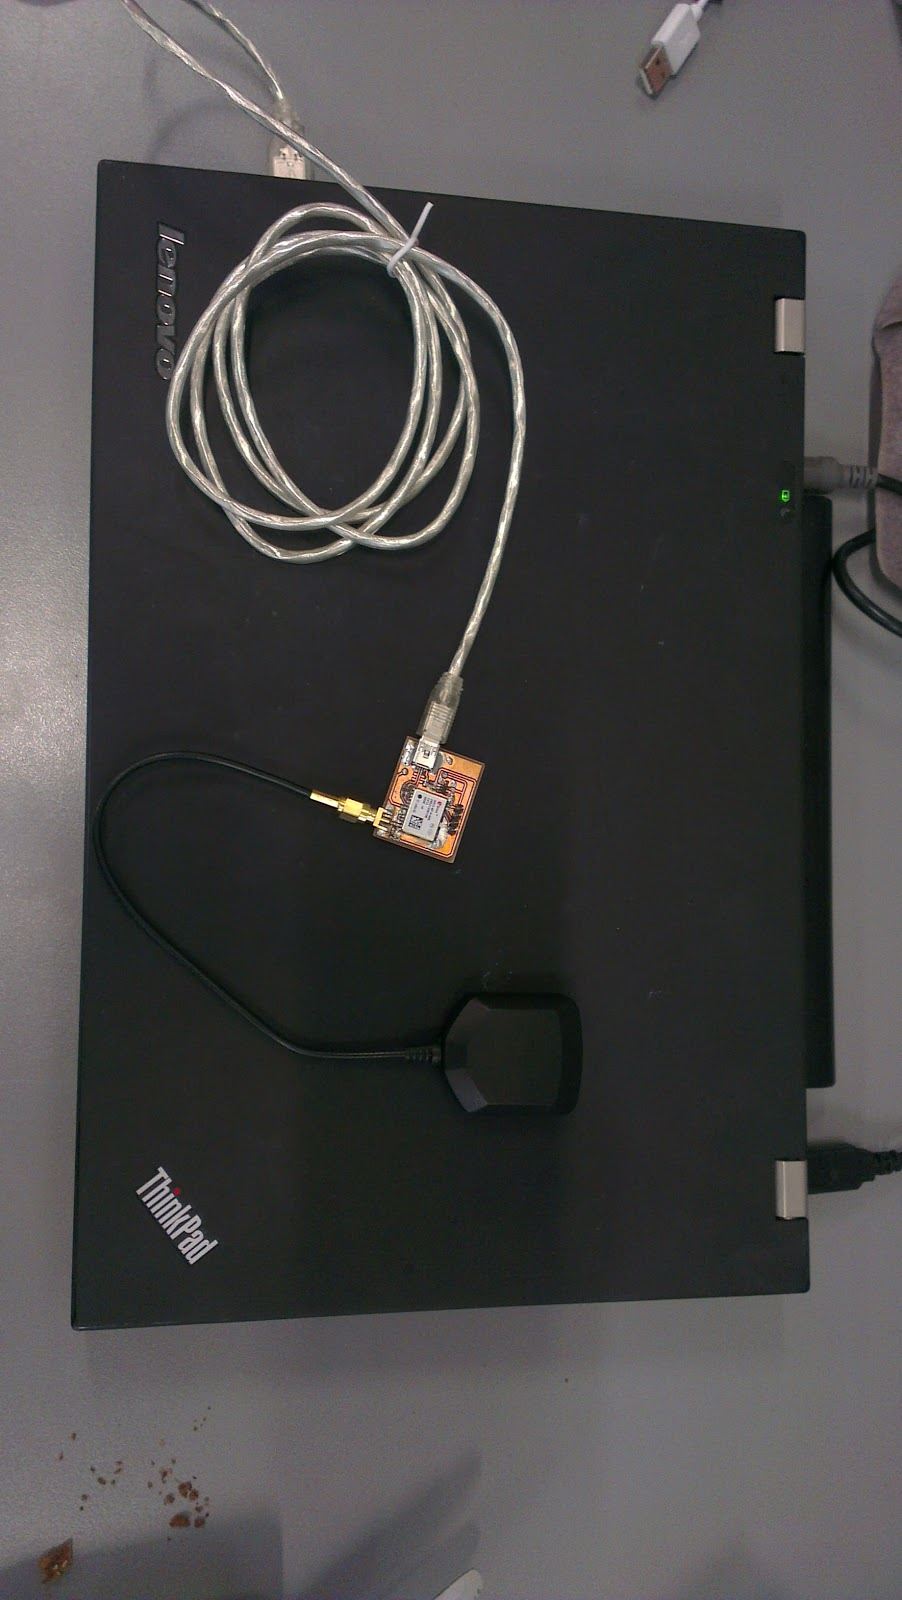
\includegraphics[width=0.5\textwidth, angle=90]{graphics/test_laptop.jpg}
  \caption[Comment]{The Neo6-P GPS (PCB developed by SDU), u-blox active GPS antenna \protect\footnote{ANNMS005} and authers laptop used in this test}   \label{fig:test_laptop_and_gps}
\end{figure}
The coordinates recorded by the rosbag is shown in figure \ref{fig:gps_raw_plot}. 
FreeNMEA\footnote{http://freenmea.net/} was used to plot the GPGGA messages obtained from the GPS.
\begin{figure}[H]
    \center
    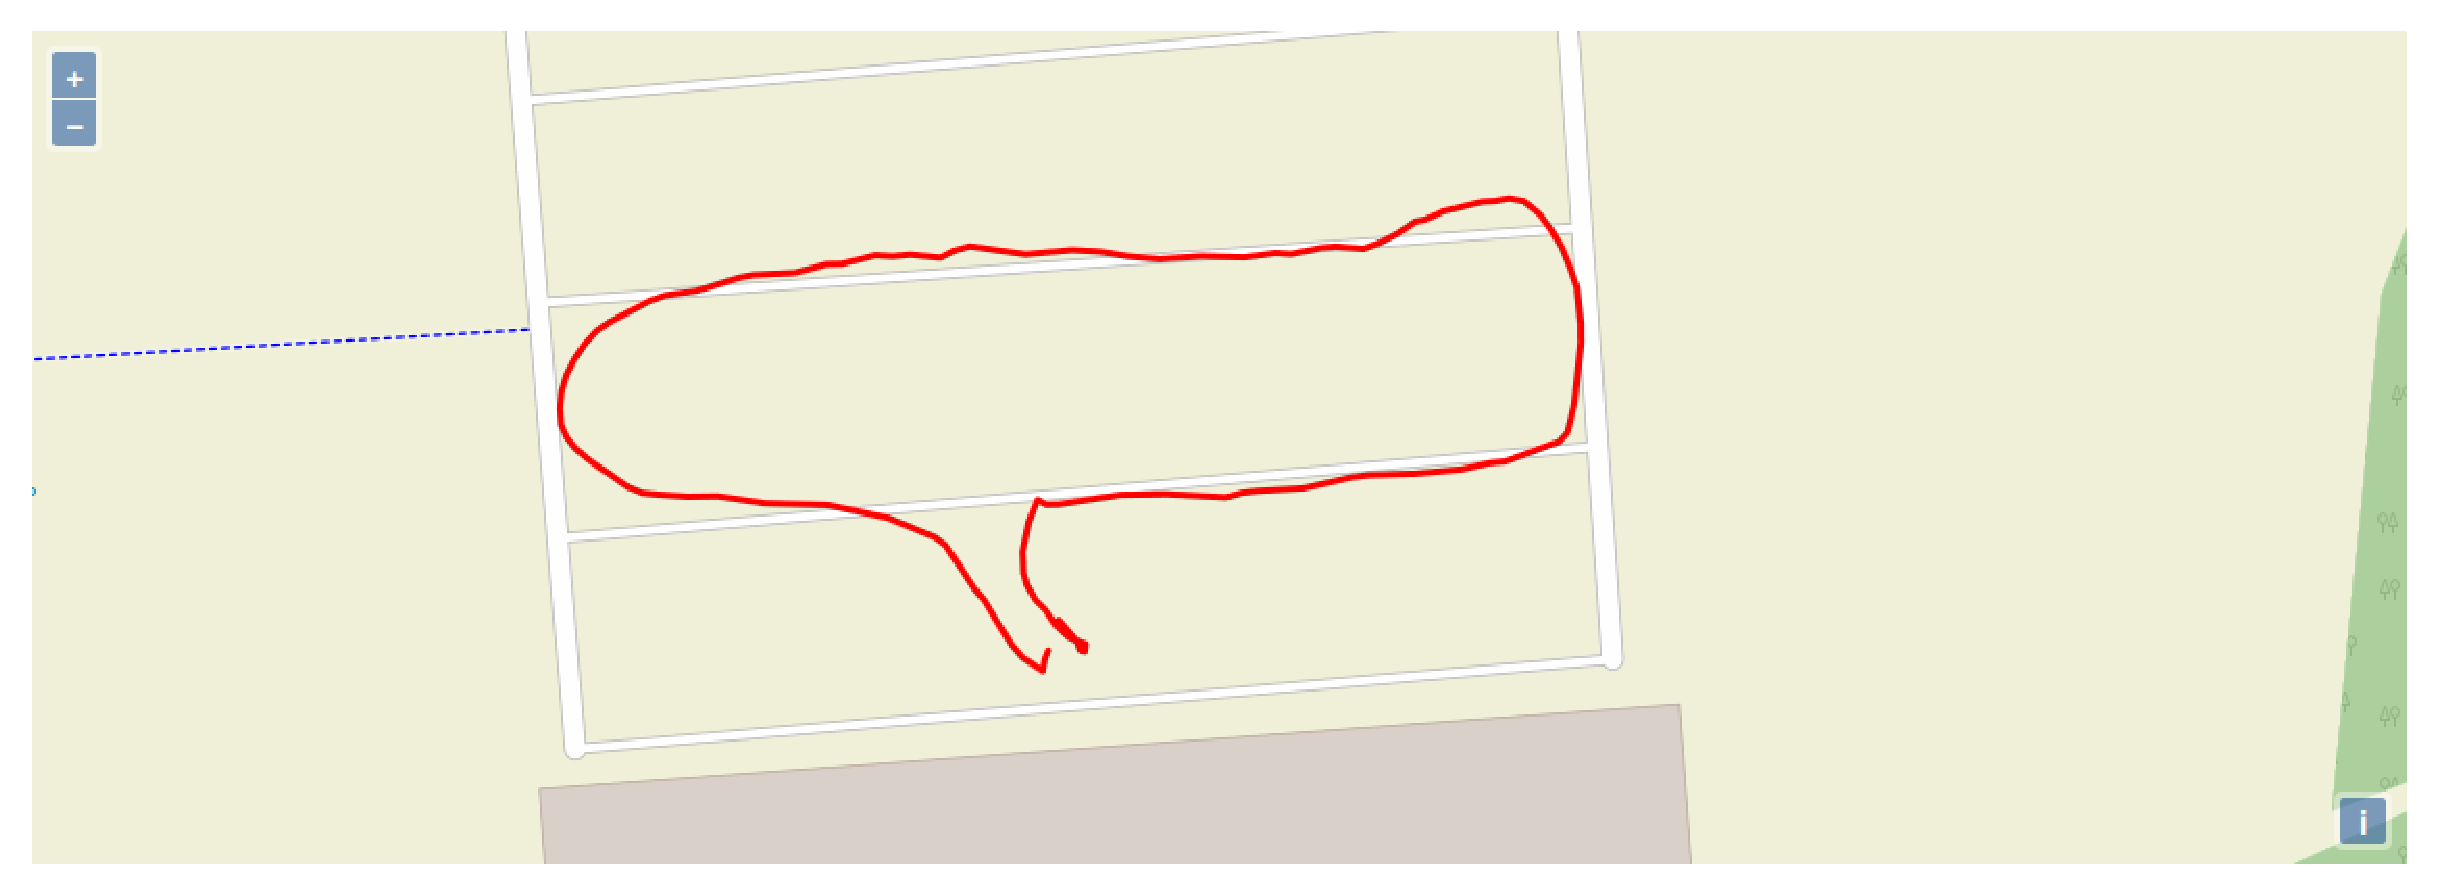
\includegraphics[width=1\textwidth]{graphics/gps_test_gps_plot}
  \caption{Test coordinates plotted}  \label{fig:gps_raw_plot}
\end{figure}
The rosbag containing the GPS coordinates where played on the Rpi, to see if the ROS node responsible for converting GPGGA messages into CAN messages were working. QgroundStation plots AQ's belief in where the drone is. The plot can be seen in figure \ref{fig:test_qground_plot}

\begin{figure}[H]
    \center
    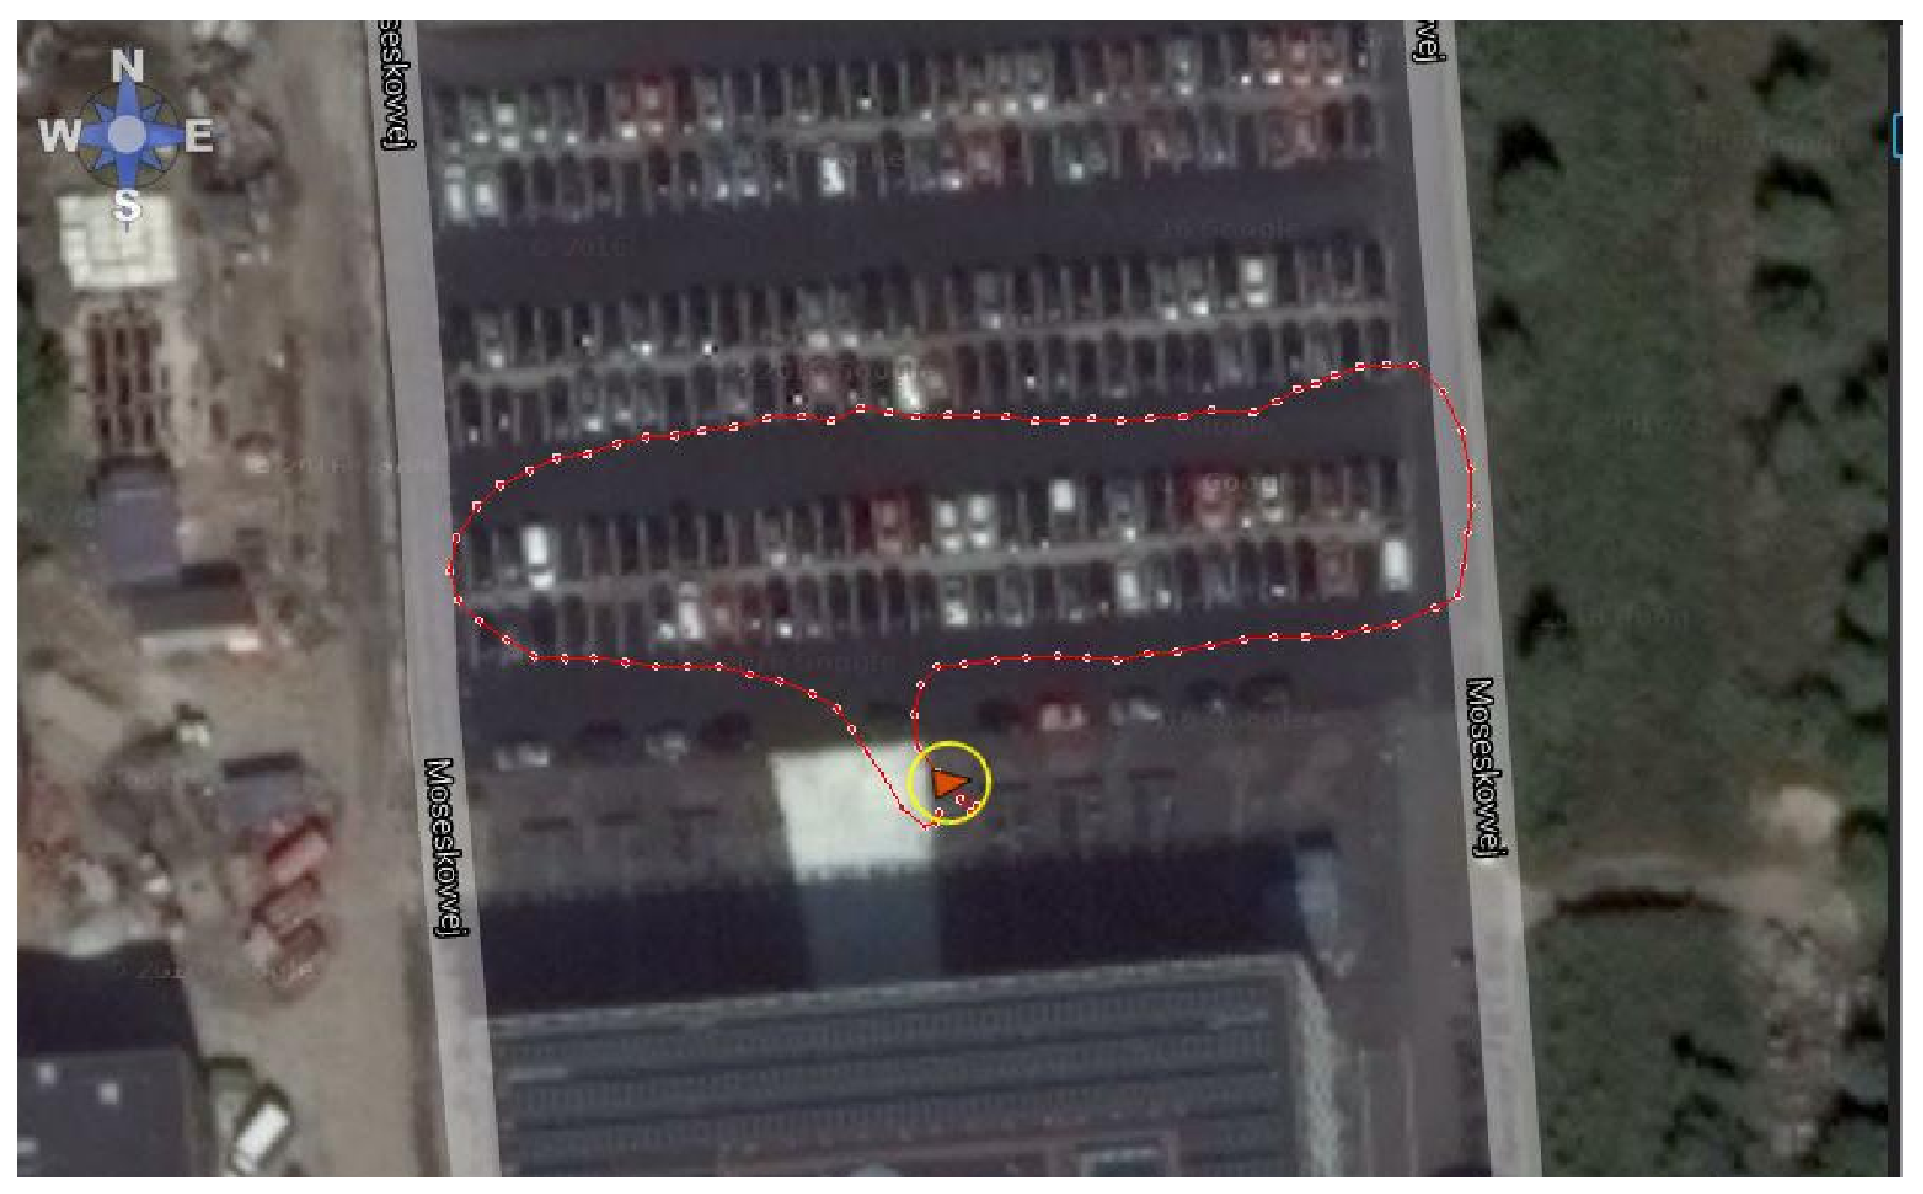
\includegraphics[width=0.8\textwidth]{graphics/test_qground_plot.eps}
  \caption{QgroundStations plot of AQ's belief in where the drone is}   \label{fig:test_qground_plot}
\end{figure}

\textbf{Conclusion}
This test visually confirms that the coordinates is spoofed correctly and read probably by AQ as long as the drone is laying on a table. Passing this test means there is reason to believe that it also works when the drone is airborne.





\subsection{Initial test flight with spoofed GPS}
\label{sec:test_of_spoofed_positions_outdoore}
\textbf{Introduction}
The purpose of this test was to see if the GPS spoofing worked when the drone was airborn. The same hardware and software were used as in section \ref{sec:test_of_spoofed_positions_indoore}, though with a few changes.

The GPS used in test 1 to collect coordinates were mounted on the EduQuad.

The idea was to pass-through the GPS coordinates from the Neo 6-P GPS to AQ. If the CAN spoofing works as expected the drone should behave normally when flying in position-hold mode.

\textbf{Test}

Figure \ref{fig:eduquad_bottom_up} shows how the hardware were mounted on the EduQuad. It was temporary mounted with strips and tape to avoid short circuiting. \Mathias{Opdater billede med test-equipment} 

In test 1 the altitude of the drone was hardcoded since it had no relevance  in the test. Though in test 2 if was necessary since the UKF\footnote{\url{https://github.com/bn999/autoquad/blob/master/onboard/run.c\#L111}} uses the altitude from the GPS to estimate the position of the drone. Furthermore the following check where inserted to make sure only valid GPS coordinates were fed into the AQ:
\begin{center}

\begin{minipage}{\textwidth}
		\begin{lstlisting}[language = c++, caption = Quality checks added to discard bad positions, label=code:pseudo_tx]
// default low accuracy
gpsData.hAcc = 5; // Meters
gpsData.vAcc = 5; // Meters

if(gpsData.fix == 1){ // Single point solution
	if(gpsData.hdop < 3){
		if(gpsData.satellites >= 5){
			AQ_PRINTF("Recv. Valid GPGGA\n",0);
			// High accuracy
			gpsData.hAcc = 2.5; // Meters
			gpsData.vAcc = 2.5; // Meters
			// Set flag to process new message
			CoSetFlag(gpsData.gpsPosFromCanFlag);
        } else {
			AQ_PRINTF("Satellites: %f \n", gpsData.satellites);       
        }
    } else {
	    AQ_PRINTF("HDOP: %f\n", gpsData.hdop);    	
    }
} else {
	AQ_PRINTF("Fix: %f\n", gpsData.fix);
}
		\end{lstlisting}
\end{minipage}
\end{center}

\begin{figure}[H]
    \center
    \includegraphics[width=0.6\textwidth]{graphics/test_outdoore_mounts.eps}
  \caption{The EduQuad drone with the hardware used in the test}
    \label{fig:eduquad_bottom_up}
\end{figure}
An extra battery was mounted on the drone to supply the Rpi. The ROS nodes running on the Rpi had to be start up before AQ starts registering notes on the CAN-bus. If the nodes was not started up, they would not reply to AQs reset-msg it sends when it is booting. \\

When the ROS-node were connected to the CAN bus, it showed that the ROS-node needed extra checking on CAN messages in order to detect difference between messages targeted the ROS-node and messages targeted the ESC32-nodes.


A bug in the \textit{can\_socketcan} -node used to communicate with the Peak-Can adapter where found a fixed. It was later on merged back into Frobomind \footnote{\url{https://github.com/FroboLab/frobomind/pull/12}}
\textbf{Conclusion} \\

The test did not go as expected. The test was carried out under a time pressure since the author's supervisor only had 30 minutes to carry out the test.

The author did though gain experience when having multiple CAN devices connected to the CAN-bus.

Several things went wrong through the test:
\begin{itemize}
	\item The onboard GPS was not disabled
	\item The author accidentally forgot to set the DOP values used in AQ
	\item No reference flight after the firmware were flashed for the first time.
	\item The GPS antenna was not mounted in the middle of the frame as the onboard antenna.
\end{itemize}

Figure \ref{fig:qground_station_dop} shows the DOP value is lowering witch indicates that AQ was using its onboard GPS.

\begin{figure}[H]
    \center
    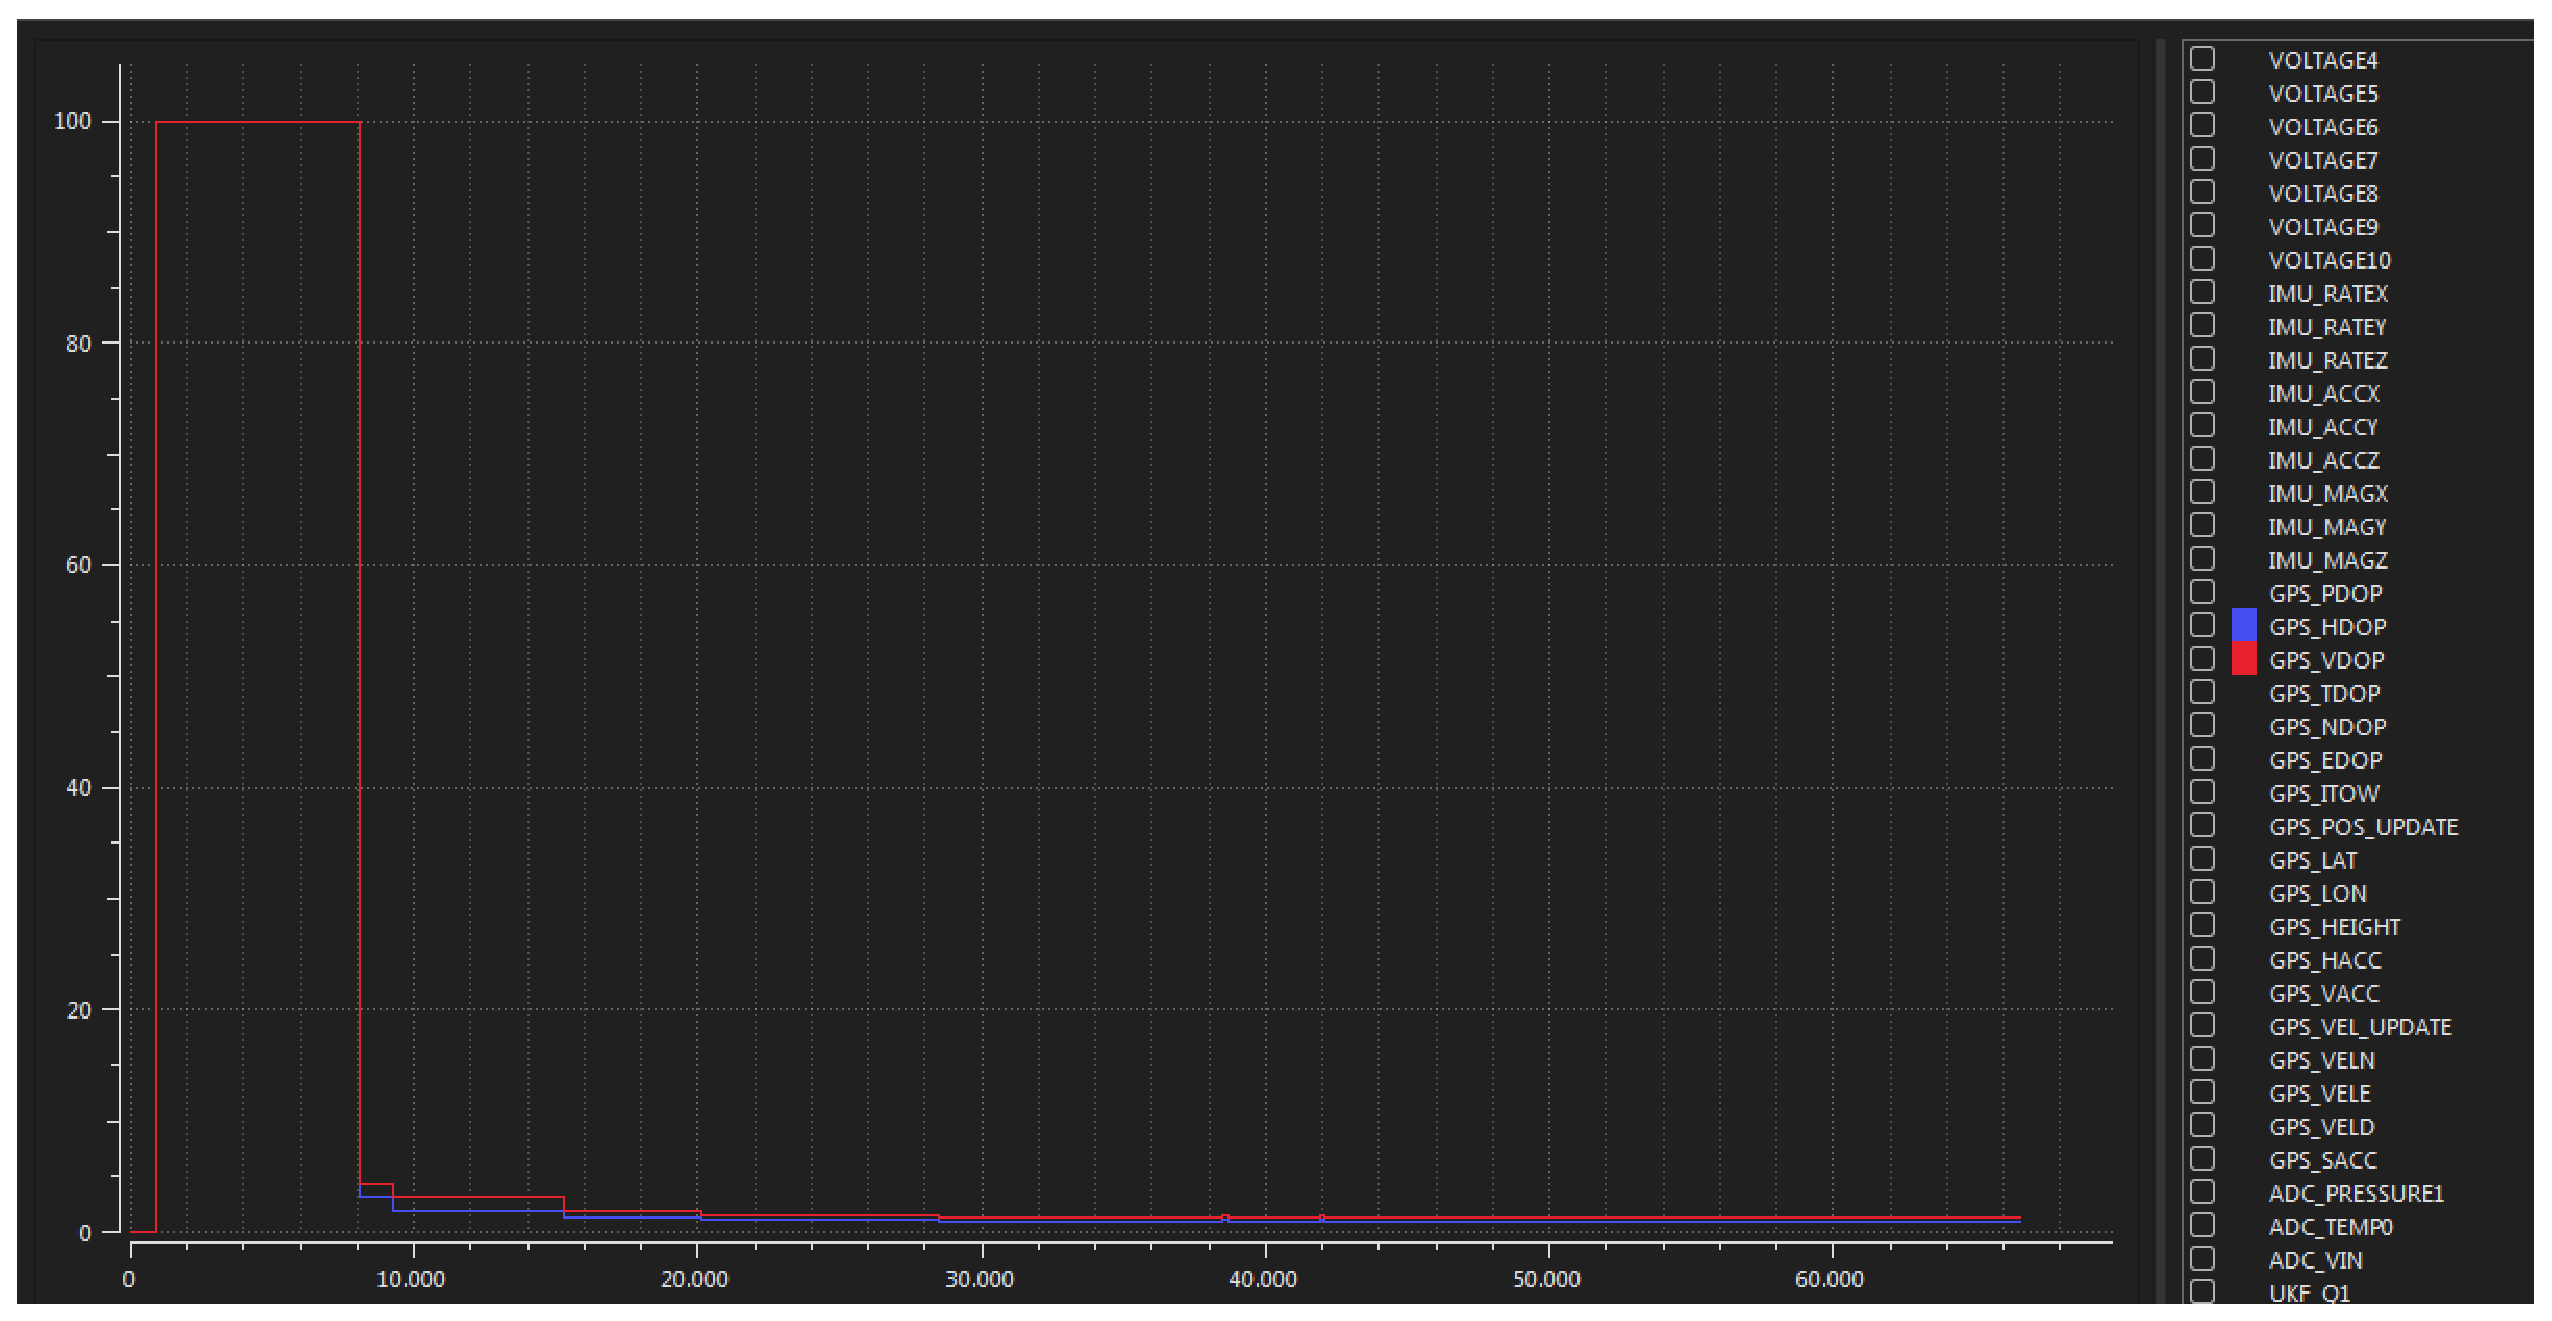
\includegraphics[width=1\textwidth]{graphics/test_qground_station_dop.eps}
  \caption{Plot of h/vDOP from logs when the drone was airborn}
    \label{fig:qground_station_dop}
\end{figure}

The test will be carried out again.


\subsection{Comparison of onboard and spoofed GPS}
\label{sec:test_of_spoofed_positions_outdoore}
\textit{This test was made together with Kjeld Jensen in order get one step further to spoofing the drones onboard GPS with an RTK GPS. A ublox Neo6-P GPS and an active <ANTENNE> was mounted on a EDUQuad drone to obtain the drone's position. A RPI was used on the EDUQuad to convert GPGGA and GPRMC from the Neo6-p GPS to CAN-mesasagess.
The test was done by walking 20 meters with the EduQuad two times to compare the output of the UKF with the different GPS's.
The values used to spoofed the GPS was found by analyzing a logfile from a regular flight to see the range of the values such as accuracy, DOP etc. when the drone was in the air. 
Values available from the Neo6-p GPS, was used directly to spoof the onboard GPS and values not available was either calculated or hardcoded.
Three tests were made due to a few code-errors but only the first and the last will be described. This test was also relevant for the indoor flying since the indoor application requires the position of the drone can be spoofed and the accuracies and DOPs can be set}\\

%\begin{wrapfigure}{r}{0.5\textwidth}
%  \begin{center}
\begin{figure}[H]
\centering
    \includegraphics[width=0.4\textwidth]	{graphics/eduquad_outdoor_flighttest_rpi_can_spoof.png}
	  \caption{Nep-6p connected to a M4 through a RPI}
    \label{fig:qground_station_dop}
\end{figure}
%  \end{wrapfigure}


In order to easily switch between the onboard GPS and the Neo-6P GPS during the test, a switch on the Spectrum DX9\footnote{\url{http://www.spektrumrc.com/Products/Default.aspx?ProdId=SPMR9900} last visited 21. Maj} was read in AutoQuad's firmware to decide which of the two GPS's data should be used. When a GPS update(time, position or velocity) is received from the onboard GPS, the struct showed in code \ref{code:gpsData_Struct} is filled in. \\


%\begin{wrapfigure}{r}{0.5\textwidth}
%  \begin{center}
\begin{lstlisting}[language = c++, caption = Quality checks added to discard bad positions, label=code:gpsData_Struct]
typedef struct {
	...
    double lat;
    double lon;
    float height;   // above mean sea level (m)
    float hAcc;     // horizontal accuracy est (m)
    float vAcc;     // vertical accuracy est (m)
    float velN;     // north velocity (m/s)
    float velE;     // east velocity (m/s)
    float velD;     // down velocity (m/s)
    float speed;    // ground speed (m/s)
    float heading;  // deg
    float sAcc;     // speed accuracy est (m/s)
    float cAcc;     // course accuracy est (deg)
    float pDOP;     // position Dilution of Precision
    float hDOP;
    float vDOP;
    float tDOP;
    float nDOP;
    float eDOP;
    float gDOP;

    //Used in GPS spoof
    uint8_t fix;
    uint8_t satellites;
    int out_cnt;

	...
} gpsStruct_t;
\end{lstlisting}
%  \end{center}
%  \end{wrapfigure}


In order to spoof the onboard GPS correctly, the author and his supervisor decided to overwrite all of the relevant elements in the struct. However, the RTC was set from the onboard GPS.

Tables \cref{tab:CAN_DOC_LAT,tab:CAN_DOC_LON,tab:CAN_DOC_VEL,tab:CAN_DOC_ALT,tab:CAN_DOC_DOP,tab:CAN_DOC_ACC} show the CAN-messages created to send data to fill in the struct.
\begin{multicols}{2}
\begin{table}[H]
	\begin{tabular}{@{}|l|l|@{}}
		\toprule
		DOC   & CAN\_DOC\_LAT \\ \midrule
		Value & Latitude      \\ \midrule
		Bits  & 63:0          \\ \bottomrule
	\end{tabular}
	\caption{CAN messages from RPI to AutoQuad containing 8 byte latitude}	\label{tab:CAN_DOC_LAT}

	\begin{tabular}{@{}|l|l|@{}}
	\toprule
		DOC   & CAN\_DOC\_LON \\ \midrule
		Value & Longitude     \\ \midrule
		Bits  & 63:0          \\ \bottomrule
	\end{tabular}
	\caption{CAN messages from RPI to AutoQuad containing 8 byte longitude} 	\label{tab:CAN_DOC_LON}

\end{table}
\columnbreak
\begin{table}[H]
	\begin{tabular}{@{}|l|l|l|l|l|@{}}
		\toprule
		DOC   & \multicolumn{4}{l|}{CAN\_DOC\_VEL} \\ \midrule
		Value & VelN    & VelE   & VelD   & speed  \\ \midrule
		Bits  & 63:48   & 47:32  & 31:16  & 15:0   \\ \bottomrule
	\end{tabular}
	\caption{CAN messages from RPI to AutoQuad containing velocities each of 2 bytes}
	\label{tab:CAN_DOC_VEL}
	\begin{tabular}{@{}|l|l|@{}}
	\toprule
		DOC   & CAN\_DOC\_ALT \\ \midrule
		Value & Altitude      \\ \midrule
		Bits  & 63:0          \\ \bottomrule
	\end{tabular}
	\caption{CAN messages from RPI to AutoQuad containing 8 byte altitude}
	\label{tab:CAN_DOC_ALT}
\end{table}
\end{multicols}

\begin{table}[H]
	\begin{tabular}{@{}|l|l|l|l|l|l|l|l|@{}}
		\toprule
		DOC   & \multicolumn{7}{l|}{CAN\_DOC\_DOP}                  \\ \midrule
		Value & gDOP  & eDOP  & nDOP  & tDOP  & vDOP  & hDOP & pDOP \\ \midrule
		Bits  & 55:48 & 47:40 & 39:32 & 31:24 & 23:16 & 15:8 & 7:0  \\ \bottomrule
	\end{tabular}
	\caption{CAN messages from RPI to AutoQuad containing DOPs each of 1 byte}
	\label{tab:CAN_DOC_DOP}
	\begin{tabular}{@{}|l|l|l|l|l|l|l|l|@{}}
		\toprule
		DOC   & \multicolumn{7}{l|}{CAN\_DOC\_ACC}                          \\ \midrule
		Value & Heading & vAcc  & hAcc  & cAcc  & sAcc  & Fix  & Satellites \\ \midrule
		Bits  & 63:48   & 47:40 & 39:32 & 31:24 & 23:16 & 15:8 & 7:0        \\ \bottomrule
	\end{tabular}\label{tab:CAN_DOC_ACC}
	\caption{CAN messages from RPI to AutoQuad containing accuracies each of 1 byte and heading in 2 bytes} 
\end{table}

In order to know the required bytes to send latitude and longitude with a precision of 1 cm, the author used the datum WGS84\footnote{WGS-84 used in AQ} to estimate the worst-case error at equator. 

WGS-84 \footnote{\url{http://www.unoosa.org/pdf/icg/2012/template/WGS_84.pdf} last visited 22 maj} states that the semi-major-axis(a) of the earth is 6378137.0 m and that the flattening factor is 1/298.257223563. From these two values the semi-minor-axis(b) can be calculated using equation \ref{eq:raduis}
\begin{equation}
b=a \cdot (1-\frac{1}{298.257223563})
\end{equation} \label{eq:raduis}
Given the formula of the circumference of an ellipsoid:
\begin{equation}
circumference = 2 \cdot \pi \sqrt{ \frac{1}{2}(a^2+b^2)}
\end{equation} \label{eq:circum}
Equation \ref{eq:circum} gives a circumference at equator of 39873752.0 meters.

By dividing 39873752.0 by 360, one get how many meters pr. degree.
\begin{equation}
\frac{39873752.0}{360} = 110760 \frac{m}{deg}
\end{equation}

Table \ref{tab:precision_latlon} was made to see how many decimals is required to obtain different precisions.
\begin{table}[H]
\centering
\caption{Table shows precision required}
\label{tab:precision_latlon}
\begin{tabular}{@{}|l|l|l|@{}}
\toprule
Decimal place & Decimal degrees & Distance    \\ \midrule
0             & 1               & 110760 m    \\ \midrule
1             & 0.1             & 11076.0 m   \\ \midrule
...           & ..              & ...         \\ \midrule
7             & 0.0000001       & 7.75323 cm  \\ \midrule
8             & 0.00000001      & 0.775323 cm \\ \bottomrule
\end{tabular}
\end{table}

It can be seen that 8'th decimal is necessary to get below 1 cm. 
To see if a float can handle number smaller than $1\cdot e-8$, \textit{eps} from MatLab was used\footnote{http://se.mathworks.com/help/matlab/ref/eps.html}.
\begin{lstlisting}[language = matlab, caption = Check if float is precise enough of a double has to be used, label=code:eps_single]
eps(single(180.0)) = 1.5259e-05
eps(double(180.0)) = 2.8422e-14
\end{lstlisting}
In code \ref{code:eps_single} eps is given with 180 as input since 180 is the largest integer possible with using latitude and longitude.
It can be seen that the smallest number a float can represent is 1.5259e-05 but a precession of $1\cdot e-8$ is needed.
However a double can easily handle that which makes the latitude and longitude of the CAN-messages 8 bytes each. \\

2 bytes are allocated for each velocity, speed and heading. In order to send 2 decimals, each value was multiplied by 100 when sending and divided by 100 when received by AutoQuad.

Only one decimal for rest of the values was deemed necessary and was thereby multiplied and divided by 10. \\

To tell the UKF in AQ how much to believe in the GPS coordinates, the onboard GPS feeds the UKF with DOP factors. The DOP factors expresses how well the satellites are placed. If they are all located around the same spot, the DOP factors will be high since the triangulation becomes less accurate. The DOP factors has no unit but is simply a scaling of the error estimate. \footcite{kelddueholmmikkellaurentziusannab.o.jensen2015}

\Mathias{Insert image from normal flight}
\newpage
Figure \ref{fig:dop_read_flight} shows a flight using onboard GPS where the DOP values where read. The values listed in table \ref{tab:DOP} was used and multiplied by the hDOP received from the Neo-6P GPS. 
\begin{wrapfigure}{r}{0.35\textwidth}
 \begin{center}
	\caption{Scaling factors used when using Neo-6p GPS}
	\label{tab:DOP}
	\begin{tabular}{@{}|l|l|@{}}
	\toprule
	Dop  & Value     \\ \midrule
	pDOP & 1.75*hdop \\ \midrule
	hDOP & 1*hdop    \\ \midrule
	vDOP & 1.5*hdop  \\ \midrule
	tDOP & 1.5*hdop  \\ \midrule
	nDOP & 0.7*hdop  \\ \midrule
	eDOP & 0.7*hdop  \\ \midrule
	gDOP & 1*hdop    \\ \bottomrule
	\end{tabular}
  \end{center}
\end{wrapfigure}

The pDOP was set to 1.75 times higher than the hDOP since it incorporates error from both vDOP and hDOP \footcite{kelddueholmmikkellaurentziusannab.o.jensen2015}. \\
vDOP is usually 1.5-2 tims higher than hDOP.  \footcite{kelddueholmmikkellaurentziusannab.o.jensen2015}. \\
tDOP was sat to 1.5 higher than hDOP since timeerror causes position error. \footnote{\url{http://www.environmental-studies.de/GPS/Dilution-of-precision/dilution-of-precision.html} last visited 22 maj} \\
Since hDOP can be split into nDOP and eDOP, they each of some of the error factor. \\
\Mathias{Gdop, skal den ikke være højere siden den har både vDOP, hDOP og tDOP} \footcite{kelddueholmmikkellaurentziusannab.o.jensen2015}




\begin{figure}[H]
\centering
    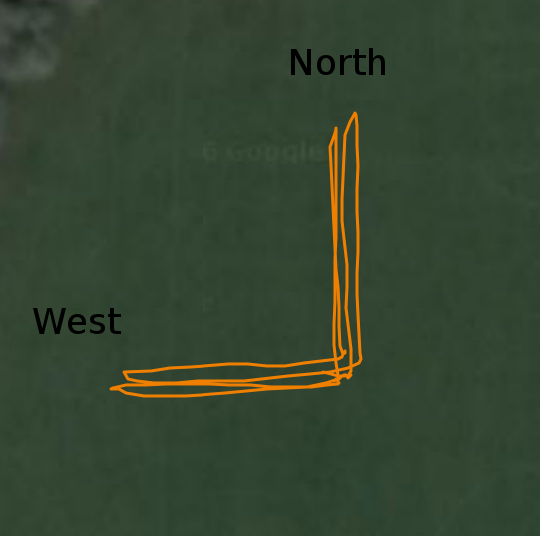
\includegraphics[width=0.4\textwidth]	{graphics/test_walked_90deg.png}
	  \caption{Path walked. If looking close it can be seen the path was walked twice, once with onboard GPS then using Neo-6p}
    \label{fig:qground_station_dop}
\end{figure}
The test was conducted by walking 20 meters \footnote{Measured by counting footsteps} north, 20 meters south, 20 meters east and 20 meters west. After walking 20 meters a small break of five seconds was held. Figure \ref{fig:position_plot} shows the walked path.
\Mathias{Figure med gpgga plot}
The coordinates plotted in figure \ref{fig:position_plot} was from the first test. Figure \ref{fig:ukf_plot} shows a plot of the position with x-axix as time.
\Mathias{Plot af northing and easting fra ukf}
Figure \ref{fig:ukf_plot} matches with the walked path seen in figure \ref{positon_plot}. The line crossing severel times is the switch on the Spectrum DX9 transmitter. It can be seen how the path repeats itself after the switch has been switched.
\Mathias{plot af pos og switch samt dop så man kan se de ændrer sig ved skift.}
Figure \ref{fig:ukf_dop} shows the same plot but where the vDOP and hDOP has been added. It can be seen when zoomed in, how the DOP values is also changing since the DOPs are higher when switching to the Neo-6p GPS.


\Mathias{Billede der viser højden/hastigheden er mere woobly siden DOP er mega lav, den stoler for meget på GPS}


Figur der viser højden samt højdehastigheden

figur der viser vele og veln der ikke virker.

Ny test, samme måde som første test, dog med følgende resultater \footnote{fejlen skyltes forkert blevev hevet ud fra C++ vector samt en variabel var brugt forkerte sted.}

\footcite{kelddueholmmikkellaurentziusannab.o.jensen2015}






\section{Documentation made throughout this thesis}
\end{document}
